% Capitolul 14: Active cripto
% Statistica piețelor financiare -- Program de licență, Academia de Studii Economice din București
% GENERAT de latex/build_chapter14.py -- modificați generatorul, nu acest fișier.

\newcommand{\coursename}{Statistica piețelor financiare}
\def\sfmlang{ro}
% Preambul comun SFM -- Statistica piețelor financiare / Statistics of Financial Markets (Beamer, 16:9)
% Același design ca MFM. Înainte de % Preambul comun SFM -- Statistica piețelor financiare / Statistics of Financial Markets (Beamer, 16:9)
% Același design ca MFM. Înainte de % Preambul comun SFM -- Statistica piețelor financiare / Statistics of Financial Markets (Beamer, 16:9)
% Același design ca MFM. Înainte de \input{../../latex/preamble} se definește
%   \newcommand{\coursename}{Statistics of Financial Markets}      (EN)
%   \newcommand{\coursename}{Statistica piețelor financiare}       (RO)  și  \def\sfmlang{ro}
% Fișierele .tex se află în EN/Courses, EN/Seminars, RO/Cursuri, RO/Seminarii (două niveluri sub rădăcină).
% Deck-urile sînt generate de latex/build_chapterN.py / build_seminarN.py (vezi latex/sfm_build.py).

\documentclass[9pt, aspectratio=169, t]{beamer}
\providecommand{\coursename}{Statistics of Financial Markets}

% Ensure content fits on slides
\setbeamersize{text margin left=8mm, text margin right=8mm}

%=============================================================================
% THEME AND STYLE CONFIGURATION
%=============================================================================
\usetheme{default}
% Using default theme for clean header/footer control

% Color Palette (matching Redispatch PDF)
\definecolor{MainBlue}{RGB}{26, 58, 110}
\definecolor{AccentBlue}{RGB}{26, 58, 110}
\definecolor{IDAred}{RGB}{205, 0, 0}
\definecolor{DarkGray}{RGB}{51, 51, 51}
\definecolor{MediumGray}{RGB}{128, 128, 128}
\definecolor{LightGray}{RGB}{248, 248, 248}
\definecolor{VeryLightGray}{RGB}{235, 235, 235}
\definecolor{KeynoteGray}{RGB}{218, 218, 218}
\definecolor{SectionGray}{RGB}{120, 120, 120}
\definecolor{FooterGray}{RGB}{100, 100, 100}
\definecolor{Crimson}{RGB}{220, 53, 69}
\definecolor{Forest}{RGB}{46, 125, 50}
\definecolor{Amber}{RGB}{181, 133, 63}
\definecolor{Orange}{RGB}{230, 126, 34}
\definecolor{Purple}{RGB}{142, 68, 173}

% Gradient background (exact Keynote 315° gradient: white to RGB 218,218,218)
\setbeamertemplate{background}{%
    \begin{tikzpicture}[remember picture, overlay]
        \shade[shading=axis, shading angle=315,
        top color=white, bottom color=KeynoteGray]
        (current page.south west) rectangle (current page.north east);
    \end{tikzpicture}%
}
% Fallback solid color for compatibility
\setbeamercolor{background canvas}{bg=}

\setbeamercolor{palette primary}{bg=MainBlue, fg=white}
\setbeamercolor{palette secondary}{bg=MainBlue!85, fg=white}
\setbeamercolor{palette tertiary}{bg=MainBlue!70, fg=white}
\setbeamercolor{structure}{fg=MainBlue}
\setbeamercolor{title}{fg=IDAred}
\setbeamercolor{frametitle}{fg=IDAred, bg=}
\setbeamercolor{block title}{bg=MainBlue, fg=white}
\setbeamercolor{block body}{bg=VeryLightGray, fg=DarkGray}
\setbeamercolor{block title alerted}{bg=Crimson, fg=white}
\setbeamercolor{block body alerted}{bg=Crimson!8, fg=DarkGray}
\setbeamercolor{block title example}{bg=Forest, fg=white}
\setbeamercolor{block body example}{bg=Forest!8, fg=DarkGray}
\setbeamercolor{item}{fg=MainBlue}

% Footer colors (override Madrid theme blue)
\setbeamercolor{author in head/foot}{fg=FooterGray, bg=}
\setbeamercolor{title in head/foot}{fg=FooterGray, bg=}
\setbeamercolor{date in head/foot}{fg=FooterGray, bg=}
\setbeamercolor{section in head/foot}{fg=FooterGray, bg=}
\setbeamercolor{subsection in head/foot}{fg=FooterGray, bg=}

% Bullet styles (apply everywhere including blocks)
\setbeamertemplate{itemize item}{\color{MainBlue}$\boxdot$}
\setbeamertemplate{itemize subitem}{\color{MainBlue}$\blacktriangleright$}
\setbeamertemplate{itemize subsubitem}{\color{MainBlue}\tiny$\bullet$}
\setbeamertemplate{itemize/enumerate body begin}{\normalsize}
\setbeamertemplate{itemize/enumerate subbody begin}{\normalsize}

% Item spacing - compact style
\setlength{\leftmargini}{10pt}       % Level 1: minimal indent
\setlength{\leftmarginii}{10pt}      % Level 2: minimal additional indent
% Compact list spacing (zero extra space before/after lists in blocks)
\makeatletter
\def\@listi{\leftmargin\leftmargini \topsep 0pt \parsep 0pt \itemsep 0pt}
\def\@listii{\leftmargin\leftmarginii \topsep 0pt \parsep 0pt \itemsep 0pt}
\makeatother

\setbeamertemplate{navigation symbols}{}

%=============================================================================
% CUSTOM HEADLINE
%=============================================================================
\setbeamertemplate{headline}{%
    \vskip10pt%
    \hbox to \paperwidth{%
        \hskip0.5cm%
        {\small\color{FooterGray}\renewcommand{\hyperlink}[2]{##2}\insertsectionhead}%
        \hfill%
        \textcolor{FooterGray}{\small\insertframenumber}%
        \hskip0.5cm%
    }%
    \vskip4pt%
    {\color{FooterGray}\hrule height 0.4pt}%
}

%=============================================================================
% CUSTOM FOOTER
%=============================================================================
\usepackage{fontawesome5}

\setbeamertemplate{footline}{%
    {\color{FooterGray}\hrule height 0.4pt}%
    \vskip4pt%
    \hbox to \paperwidth{%
        \hskip0.5cm%
        \textcolor{FooterGray}{\small\coursename}%
        \hfill%
        \raisebox{-0.1em}{%
            \begin{tikzpicture}[x=0.08em, y=0.08em, line width=0.4pt]
                \draw[FooterGray] (0,3) -- (1,4) -- (2,3.5) -- (3,5) -- (4,4) -- (5,6) -- (6,5.5) -- (7,4) -- (8,5) -- (9,7) -- (10,6) -- (11,5) -- (12,6.5) -- (13,8) -- (14,7) -- (15,6) -- (16,7.5) -- (17,9) -- (18,8) -- (19,7) -- (20,8.5) -- (21,10) -- (22,9) -- (23,8) -- (24,9.5);
            \end{tikzpicture}%
        }%
        \hskip0.5cm%
    }%
    \vskip6pt%
}

%=============================================================================
% PACKAGES
%=============================================================================
\usepackage[utf8]{inputenc}
\DeclareUnicodeCharacter{03B1}{\ensuremath{\alpha}}
\usepackage[T1]{fontenc}
\usepackage{amsmath, amssymb, amsthm}
\usepackage{mathtools}
\usepackage{bm}
\usepackage{tikz}
\usetikzlibrary{arrows.meta, positioning, shapes, calc, decorations.pathreplacing, shadings}
\usepackage{booktabs}
\usepackage{multirow}
\usepackage{array}
\usepackage{graphicx}
\usepackage{hyperref}
\usepackage{colortbl}
\usepackage{listings}
\lstset{language=Python, basicstyle=\ttfamily\scriptsize, keywordstyle=\color{MainBlue}\bfseries,
  commentstyle=\color{Forest}, stringstyle=\color{Crimson}, breaklines=true,
  frame=none, backgroundcolor=\color{VeryLightGray}, xleftmargin=2mm}
\hypersetup{colorlinks=true, linkcolor=MainBlue, urlcolor=MainBlue}
\graphicspath{{../../logos/}{../../charts/}{../../photos/}}
\usepackage{xcolor}
\hfuzz=2pt  % Suppress tiny overfull warnings (<2pt)
\vfuzz=2pt  % Suppress tiny vertical overfull warnings (<2pt)

%=============================================================================
% QUANTLET COMMANDS
%   \quantlet{<displayed name>}{<url>}       (generic, compatible with the older SFM decks)
%   \sfmquantlet{Ch_05}{SFM_ch5_garch}       -> https://github.com/danpele/SFM/tree/main/Quantlets/Ch_05/SFM_ch5_garch
%   \qlurl{<folder>} is defined per chapter by the generator (Quantlets/Ch_NN/<folder>)
%=============================================================================
\newcommand{\sfmrepo}{https://github.com/danpele/SFM}
\newcommand{\sfmqlbase}{https://github.com/danpele/SFM/tree/main/Quantlets}
\newcommand{\quantlet}[2]{%
    \hfill\href{#2}{%
        \raisebox{-0.15em}{
\includegraphics[height=0.7em]{ql_logo.png}}%
        \textcolor{MainBlue}{\tiny\ #1}%
    }%
}
\newcommand{\sfmquantlet}[2]{\quantlet{\detokenize{#2}}{\sfmqlbase/#1/#2}}

%=============================================================================
% NOTEBOOKS (Google Colab)
%   \colaburl{notebooks/EN/chapter5_seminar_notebook.ipynb} -> the Colab link of a file in the SFM repo
%   \nb: the chapter notebook (each seminar deck redefines it with \renewcommand)
%=============================================================================
\newcommand{\colaburl}[1]{https://colab.research.google.com/github/danpele/SFM/blob/main/#1}
\newcommand{\nb}{https://colab.research.google.com/github/danpele/SFM/tree/main/notebooks/EN}
\newcommand{\nbname}{notebooks/EN}

%=============================================================================
% SLIDE HELPERS (used by the generators; the same as in MFM)
%=============================================================================
% local font size for list bodies (the preamble forces \normalsize)
\newcommand{\itemsize}[1]{\setbeamertemplate{itemize/enumerate body begin}{#1}\setbeamertemplate{itemize/enumerate subbody begin}{#1}}
\newcommand{\intitle}[1]{{\hypersetup{urlcolor=white}#1}}   % white links inside coloured title bars
\newcommand{\imgcap}[1]{{\scriptsize #1}\\[0.5mm]}          % caption under a photo
\newcommand{\imgcredit}[2]{{\tiny\color{FooterGray}\href{#1}{#2}}}   % image credit: source URL, author/licence
\newcommand{\aiprompt}[1]{{\ttfamily\color{MainBlue}#1}}     % a prompt to an AI assistant

%=============================================================================
% SEMINARS: student version by default; the instructor wrapper *_solutions.tex sets \solutionstrue
%=============================================================================
\makeatletter\@ifundefined{ifsolutions}{\expandafter\newif\csname ifsolutions\endcsname}{}\makeatother
\newcommand{\solonly}[1]{\ifsolutions #1\fi}
\newcommand{\propsub}{\ifsolutions\else\framesubtitle{\ifdefined\sfmlang Rezolvarea se discută la seminar\else Solution discussed in class\fi}\fi}

%=============================================================================
% APPENDIX AND CHAPTER LINKS (latex/appendix_links.py writes the calls; it also re-declares these
% macros before \begin{document}, so the decks compile with or without this preamble block)
%=============================================================================
\providecommand{\sfmapplink}[3]{\hypertarget{#2}{}\hyperlink{#1}{\beamergotobutton{#3}}}
\providecommand{\sfmappback}[2]{\begin{tikzpicture}[remember picture,overlay]\node[anchor=south east] at ([xshift=-3mm,yshift=7mm]current page.south east){\hyperlink{#1}{\beamerreturnbutton{#2}}};\end{tikzpicture}}
\providecommand{\sfmchlink}[2]{\href{#1}{#2}}
\providecommand{\sfmchlinkt}[2]{\href{#1}{\usebeamercolor[fg]{frametitle}#2}}

%=============================================================================
% QUANTINAR COMMAND: link către un curs Quantinar (subiecte avansate)
%=============================================================================
\newcommand{\quantinar}[2]{%
    \href{#2}{%
        \raisebox{-0.15em}{
\includegraphics[height=0.8em]{qr_logo.png}}%
        \textcolor{MainBlue}{\scriptsize\ #1}%
    }%
}

%=============================================================================
% CUSTOM TITLE PAGE
%=============================================================================
\defbeamertemplate*{title page}{hybrid}[1][]
{
    \vspace{0.2cm}
    % Logos row - top header (with clickable links)
    \begin{center}
        \href{https://www.ase.ro}{
\includegraphics[height=1.0cm]{ase_logo.png}}\hspace{0.3cm}%
        \href{https://theida.net}{
\includegraphics[height=1.0cm]{ida_logo.png}}\hspace{0.3cm}%
        \href{https://blockchain-research-center.com}{
\includegraphics[height=1.0cm]{brc_logo.png}}\hspace{0.3cm}%
        \href{https://www.ai4efin.ase.ro}{
\includegraphics[height=1.0cm]{ai4efin_logo.png}}\hspace{0.3cm}%
        \href{https://ipe.ro/new}{
\includegraphics[height=1.0cm]{acad_logo.png}}\hspace{0.3cm}%
        \href{https://www.digital-finance-msca.com}{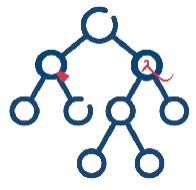
\includegraphics[height=1.0cm]{msca_logo.png}}%
    \end{center}

    \vspace{0.6cm}

    % Main title with Q logos on sides (with clickable links)
    \begin{center}
        \begin{minipage}{0.1\textwidth}
            \centering
            \href{https://quantlet.com}{
\includegraphics[height=1.1cm]{ql_logo.png}}
        \end{minipage}%
        \begin{minipage}{0.78\textwidth}
            \centering
            {\LARGE\bfseries\usebeamercolor[fg]{title}\inserttitle}

            \vspace{0.3cm}

            {\usebeamerfont{subtitle}\usebeamercolor[fg]{title}\insertsubtitle}
        \end{minipage}%
        \begin{minipage}{0.1\textwidth}
            \centering
            \href{https://quantinar.com}{
\includegraphics[height=1.1cm]{qr_logo.png}}
        \end{minipage}
    \end{center}

    \vspace{0.6cm}

    % Authors (left aligned)
    \hspace{0.5cm}{\usebeamerfont{author}\insertauthor}

    \vspace{0.3cm}

    % Institute/Affiliations (left aligned)
    \hspace{0.5cm}\begin{minipage}[t]{0.9\textwidth}
        \raggedright\small\insertinstitute
    \end{minipage}
}

%=============================================================================
% THEOREM ENVIRONMENTS
%=============================================================================
\theoremstyle{definition}
\setbeamertemplate{theorems}[numbered]
\ifdefined\sfmlang
\newtheorem{defn}{Definiție}
\newtheorem{thm}{Teoremă}
\newtheorem{prop}{Propoziție}
\newtheorem{rmk}{Observație}
\else
\newtheorem{defn}{Definition}
\newtheorem{thm}{Theorem}
\newtheorem{prop}{Proposition}
\newtheorem{rmk}{Remark}
\fi

%=============================================================================
% CENTRED MINIPAGE (no extra vertical space)
%=============================================================================
\newenvironment{cminipage}[1]{%
    \par\noindent\hfill\begin{minipage}{#1}\ignorespaces
}{%
    \end{minipage}\hfill\null\par
}

%=============================================================================
% CUSTOM COMMANDS
%=============================================================================
\newcommand{\E}{\mathbb{E}}
\newcommand{\Var}{\text{Var}}
\newcommand{\Cov}{\text{Cov}}
\newcommand{\Corr}{\text{Corr}}
\newcommand{\R}{\mathbb{R}}
\newcommand{\N}{\mathbb{N}}
\newcommand{\Z}{\mathbb{Z}}
\newcommand{\B}{\mathbf{B}}
\newcommand{\imark}{\textcolor{MainBlue}{\textbullet}}
\newcommand{\RMSE}{\text{RMSE}}
\newcommand{\MAE}{\text{MAE}}
\newcommand{\MAPE}{\text{MAPE}}

 se definește
%   \newcommand{\coursename}{Statistics of Financial Markets}      (EN)
%   \newcommand{\coursename}{Statistica piețelor financiare}       (RO)  și  \def\sfmlang{ro}
% Fișierele .tex se află în EN/Courses, EN/Seminars, RO/Cursuri, RO/Seminarii (două niveluri sub rădăcină).
% Deck-urile sînt generate de latex/build_chapterN.py / build_seminarN.py (vezi latex/sfm_build.py).

\documentclass[9pt, aspectratio=169, t]{beamer}
\providecommand{\coursename}{Statistics of Financial Markets}

% Ensure content fits on slides
\setbeamersize{text margin left=8mm, text margin right=8mm}

%=============================================================================
% THEME AND STYLE CONFIGURATION
%=============================================================================
\usetheme{default}
% Using default theme for clean header/footer control

% Color Palette (matching Redispatch PDF)
\definecolor{MainBlue}{RGB}{26, 58, 110}
\definecolor{AccentBlue}{RGB}{26, 58, 110}
\definecolor{IDAred}{RGB}{205, 0, 0}
\definecolor{DarkGray}{RGB}{51, 51, 51}
\definecolor{MediumGray}{RGB}{128, 128, 128}
\definecolor{LightGray}{RGB}{248, 248, 248}
\definecolor{VeryLightGray}{RGB}{235, 235, 235}
\definecolor{KeynoteGray}{RGB}{218, 218, 218}
\definecolor{SectionGray}{RGB}{120, 120, 120}
\definecolor{FooterGray}{RGB}{100, 100, 100}
\definecolor{Crimson}{RGB}{220, 53, 69}
\definecolor{Forest}{RGB}{46, 125, 50}
\definecolor{Amber}{RGB}{181, 133, 63}
\definecolor{Orange}{RGB}{230, 126, 34}
\definecolor{Purple}{RGB}{142, 68, 173}

% Gradient background (exact Keynote 315° gradient: white to RGB 218,218,218)
\setbeamertemplate{background}{%
    \begin{tikzpicture}[remember picture, overlay]
        \shade[shading=axis, shading angle=315,
        top color=white, bottom color=KeynoteGray]
        (current page.south west) rectangle (current page.north east);
    \end{tikzpicture}%
}
% Fallback solid color for compatibility
\setbeamercolor{background canvas}{bg=}

\setbeamercolor{palette primary}{bg=MainBlue, fg=white}
\setbeamercolor{palette secondary}{bg=MainBlue!85, fg=white}
\setbeamercolor{palette tertiary}{bg=MainBlue!70, fg=white}
\setbeamercolor{structure}{fg=MainBlue}
\setbeamercolor{title}{fg=IDAred}
\setbeamercolor{frametitle}{fg=IDAred, bg=}
\setbeamercolor{block title}{bg=MainBlue, fg=white}
\setbeamercolor{block body}{bg=VeryLightGray, fg=DarkGray}
\setbeamercolor{block title alerted}{bg=Crimson, fg=white}
\setbeamercolor{block body alerted}{bg=Crimson!8, fg=DarkGray}
\setbeamercolor{block title example}{bg=Forest, fg=white}
\setbeamercolor{block body example}{bg=Forest!8, fg=DarkGray}
\setbeamercolor{item}{fg=MainBlue}

% Footer colors (override Madrid theme blue)
\setbeamercolor{author in head/foot}{fg=FooterGray, bg=}
\setbeamercolor{title in head/foot}{fg=FooterGray, bg=}
\setbeamercolor{date in head/foot}{fg=FooterGray, bg=}
\setbeamercolor{section in head/foot}{fg=FooterGray, bg=}
\setbeamercolor{subsection in head/foot}{fg=FooterGray, bg=}

% Bullet styles (apply everywhere including blocks)
\setbeamertemplate{itemize item}{\color{MainBlue}$\boxdot$}
\setbeamertemplate{itemize subitem}{\color{MainBlue}$\blacktriangleright$}
\setbeamertemplate{itemize subsubitem}{\color{MainBlue}\tiny$\bullet$}
\setbeamertemplate{itemize/enumerate body begin}{\normalsize}
\setbeamertemplate{itemize/enumerate subbody begin}{\normalsize}

% Item spacing - compact style
\setlength{\leftmargini}{10pt}       % Level 1: minimal indent
\setlength{\leftmarginii}{10pt}      % Level 2: minimal additional indent
% Compact list spacing (zero extra space before/after lists in blocks)
\makeatletter
\def\@listi{\leftmargin\leftmargini \topsep 0pt \parsep 0pt \itemsep 0pt}
\def\@listii{\leftmargin\leftmarginii \topsep 0pt \parsep 0pt \itemsep 0pt}
\makeatother

\setbeamertemplate{navigation symbols}{}

%=============================================================================
% CUSTOM HEADLINE
%=============================================================================
\setbeamertemplate{headline}{%
    \vskip10pt%
    \hbox to \paperwidth{%
        \hskip0.5cm%
        {\small\color{FooterGray}\renewcommand{\hyperlink}[2]{##2}\insertsectionhead}%
        \hfill%
        \textcolor{FooterGray}{\small\insertframenumber}%
        \hskip0.5cm%
    }%
    \vskip4pt%
    {\color{FooterGray}\hrule height 0.4pt}%
}

%=============================================================================
% CUSTOM FOOTER
%=============================================================================
\usepackage{fontawesome5}

\setbeamertemplate{footline}{%
    {\color{FooterGray}\hrule height 0.4pt}%
    \vskip4pt%
    \hbox to \paperwidth{%
        \hskip0.5cm%
        \textcolor{FooterGray}{\small\coursename}%
        \hfill%
        \raisebox{-0.1em}{%
            \begin{tikzpicture}[x=0.08em, y=0.08em, line width=0.4pt]
                \draw[FooterGray] (0,3) -- (1,4) -- (2,3.5) -- (3,5) -- (4,4) -- (5,6) -- (6,5.5) -- (7,4) -- (8,5) -- (9,7) -- (10,6) -- (11,5) -- (12,6.5) -- (13,8) -- (14,7) -- (15,6) -- (16,7.5) -- (17,9) -- (18,8) -- (19,7) -- (20,8.5) -- (21,10) -- (22,9) -- (23,8) -- (24,9.5);
            \end{tikzpicture}%
        }%
        \hskip0.5cm%
    }%
    \vskip6pt%
}

%=============================================================================
% PACKAGES
%=============================================================================
\usepackage[utf8]{inputenc}
\DeclareUnicodeCharacter{03B1}{\ensuremath{\alpha}}
\usepackage[T1]{fontenc}
\usepackage{amsmath, amssymb, amsthm}
\usepackage{mathtools}
\usepackage{bm}
\usepackage{tikz}
\usetikzlibrary{arrows.meta, positioning, shapes, calc, decorations.pathreplacing, shadings}
\usepackage{booktabs}
\usepackage{multirow}
\usepackage{array}
\usepackage{graphicx}
\usepackage{hyperref}
\usepackage{colortbl}
\usepackage{listings}
\lstset{language=Python, basicstyle=\ttfamily\scriptsize, keywordstyle=\color{MainBlue}\bfseries,
  commentstyle=\color{Forest}, stringstyle=\color{Crimson}, breaklines=true,
  frame=none, backgroundcolor=\color{VeryLightGray}, xleftmargin=2mm}
\hypersetup{colorlinks=true, linkcolor=MainBlue, urlcolor=MainBlue}
\graphicspath{{../../logos/}{../../charts/}{../../photos/}}
\usepackage{xcolor}
\hfuzz=2pt  % Suppress tiny overfull warnings (<2pt)
\vfuzz=2pt  % Suppress tiny vertical overfull warnings (<2pt)

%=============================================================================
% QUANTLET COMMANDS
%   \quantlet{<displayed name>}{<url>}       (generic, compatible with the older SFM decks)
%   \sfmquantlet{Ch_05}{SFM_ch5_garch}       -> https://github.com/danpele/SFM/tree/main/Quantlets/Ch_05/SFM_ch5_garch
%   \qlurl{<folder>} is defined per chapter by the generator (Quantlets/Ch_NN/<folder>)
%=============================================================================
\newcommand{\sfmrepo}{https://github.com/danpele/SFM}
\newcommand{\sfmqlbase}{https://github.com/danpele/SFM/tree/main/Quantlets}
\newcommand{\quantlet}[2]{%
    \hfill\href{#2}{%
        \raisebox{-0.15em}{
\includegraphics[height=0.7em]{ql_logo.png}}%
        \textcolor{MainBlue}{\tiny\ #1}%
    }%
}
\newcommand{\sfmquantlet}[2]{\quantlet{\detokenize{#2}}{\sfmqlbase/#1/#2}}

%=============================================================================
% NOTEBOOKS (Google Colab)
%   \colaburl{notebooks/EN/chapter5_seminar_notebook.ipynb} -> the Colab link of a file in the SFM repo
%   \nb: the chapter notebook (each seminar deck redefines it with \renewcommand)
%=============================================================================
\newcommand{\colaburl}[1]{https://colab.research.google.com/github/danpele/SFM/blob/main/#1}
\newcommand{\nb}{https://colab.research.google.com/github/danpele/SFM/tree/main/notebooks/EN}
\newcommand{\nbname}{notebooks/EN}

%=============================================================================
% SLIDE HELPERS (used by the generators; the same as in MFM)
%=============================================================================
% local font size for list bodies (the preamble forces \normalsize)
\newcommand{\itemsize}[1]{\setbeamertemplate{itemize/enumerate body begin}{#1}\setbeamertemplate{itemize/enumerate subbody begin}{#1}}
\newcommand{\intitle}[1]{{\hypersetup{urlcolor=white}#1}}   % white links inside coloured title bars
\newcommand{\imgcap}[1]{{\scriptsize #1}\\[0.5mm]}          % caption under a photo
\newcommand{\imgcredit}[2]{{\tiny\color{FooterGray}\href{#1}{#2}}}   % image credit: source URL, author/licence
\newcommand{\aiprompt}[1]{{\ttfamily\color{MainBlue}#1}}     % a prompt to an AI assistant

%=============================================================================
% SEMINARS: student version by default; the instructor wrapper *_solutions.tex sets \solutionstrue
%=============================================================================
\makeatletter\@ifundefined{ifsolutions}{\expandafter\newif\csname ifsolutions\endcsname}{}\makeatother
\newcommand{\solonly}[1]{\ifsolutions #1\fi}
\newcommand{\propsub}{\ifsolutions\else\framesubtitle{\ifdefined\sfmlang Rezolvarea se discută la seminar\else Solution discussed in class\fi}\fi}

%=============================================================================
% APPENDIX AND CHAPTER LINKS (latex/appendix_links.py writes the calls; it also re-declares these
% macros before \begin{document}, so the decks compile with or without this preamble block)
%=============================================================================
\providecommand{\sfmapplink}[3]{\hypertarget{#2}{}\hyperlink{#1}{\beamergotobutton{#3}}}
\providecommand{\sfmappback}[2]{\begin{tikzpicture}[remember picture,overlay]\node[anchor=south east] at ([xshift=-3mm,yshift=7mm]current page.south east){\hyperlink{#1}{\beamerreturnbutton{#2}}};\end{tikzpicture}}
\providecommand{\sfmchlink}[2]{\href{#1}{#2}}
\providecommand{\sfmchlinkt}[2]{\href{#1}{\usebeamercolor[fg]{frametitle}#2}}

%=============================================================================
% QUANTINAR COMMAND: link către un curs Quantinar (subiecte avansate)
%=============================================================================
\newcommand{\quantinar}[2]{%
    \href{#2}{%
        \raisebox{-0.15em}{
\includegraphics[height=0.8em]{qr_logo.png}}%
        \textcolor{MainBlue}{\scriptsize\ #1}%
    }%
}

%=============================================================================
% CUSTOM TITLE PAGE
%=============================================================================
\defbeamertemplate*{title page}{hybrid}[1][]
{
    \vspace{0.2cm}
    % Logos row - top header (with clickable links)
    \begin{center}
        \href{https://www.ase.ro}{
\includegraphics[height=1.0cm]{ase_logo.png}}\hspace{0.3cm}%
        \href{https://theida.net}{
\includegraphics[height=1.0cm]{ida_logo.png}}\hspace{0.3cm}%
        \href{https://blockchain-research-center.com}{
\includegraphics[height=1.0cm]{brc_logo.png}}\hspace{0.3cm}%
        \href{https://www.ai4efin.ase.ro}{
\includegraphics[height=1.0cm]{ai4efin_logo.png}}\hspace{0.3cm}%
        \href{https://ipe.ro/new}{
\includegraphics[height=1.0cm]{acad_logo.png}}\hspace{0.3cm}%
        \href{https://www.digital-finance-msca.com}{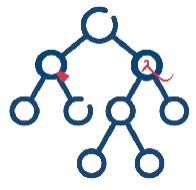
\includegraphics[height=1.0cm]{msca_logo.png}}%
    \end{center}

    \vspace{0.6cm}

    % Main title with Q logos on sides (with clickable links)
    \begin{center}
        \begin{minipage}{0.1\textwidth}
            \centering
            \href{https://quantlet.com}{
\includegraphics[height=1.1cm]{ql_logo.png}}
        \end{minipage}%
        \begin{minipage}{0.78\textwidth}
            \centering
            {\LARGE\bfseries\usebeamercolor[fg]{title}\inserttitle}

            \vspace{0.3cm}

            {\usebeamerfont{subtitle}\usebeamercolor[fg]{title}\insertsubtitle}
        \end{minipage}%
        \begin{minipage}{0.1\textwidth}
            \centering
            \href{https://quantinar.com}{
\includegraphics[height=1.1cm]{qr_logo.png}}
        \end{minipage}
    \end{center}

    \vspace{0.6cm}

    % Authors (left aligned)
    \hspace{0.5cm}{\usebeamerfont{author}\insertauthor}

    \vspace{0.3cm}

    % Institute/Affiliations (left aligned)
    \hspace{0.5cm}\begin{minipage}[t]{0.9\textwidth}
        \raggedright\small\insertinstitute
    \end{minipage}
}

%=============================================================================
% THEOREM ENVIRONMENTS
%=============================================================================
\theoremstyle{definition}
\setbeamertemplate{theorems}[numbered]
\ifdefined\sfmlang
\newtheorem{defn}{Definiție}
\newtheorem{thm}{Teoremă}
\newtheorem{prop}{Propoziție}
\newtheorem{rmk}{Observație}
\else
\newtheorem{defn}{Definition}
\newtheorem{thm}{Theorem}
\newtheorem{prop}{Proposition}
\newtheorem{rmk}{Remark}
\fi

%=============================================================================
% CENTRED MINIPAGE (no extra vertical space)
%=============================================================================
\newenvironment{cminipage}[1]{%
    \par\noindent\hfill\begin{minipage}{#1}\ignorespaces
}{%
    \end{minipage}\hfill\null\par
}

%=============================================================================
% CUSTOM COMMANDS
%=============================================================================
\newcommand{\E}{\mathbb{E}}
\newcommand{\Var}{\text{Var}}
\newcommand{\Cov}{\text{Cov}}
\newcommand{\Corr}{\text{Corr}}
\newcommand{\R}{\mathbb{R}}
\newcommand{\N}{\mathbb{N}}
\newcommand{\Z}{\mathbb{Z}}
\newcommand{\B}{\mathbf{B}}
\newcommand{\imark}{\textcolor{MainBlue}{\textbullet}}
\newcommand{\RMSE}{\text{RMSE}}
\newcommand{\MAE}{\text{MAE}}
\newcommand{\MAPE}{\text{MAPE}}

 se definește
%   \newcommand{\coursename}{Statistics of Financial Markets}      (EN)
%   \newcommand{\coursename}{Statistica piețelor financiare}       (RO)  și  \def\sfmlang{ro}
% Fișierele .tex se află în EN/Courses, EN/Seminars, RO/Cursuri, RO/Seminarii (două niveluri sub rădăcină).
% Deck-urile sînt generate de latex/build_chapterN.py / build_seminarN.py (vezi latex/sfm_build.py).

\documentclass[9pt, aspectratio=169, t]{beamer}
\providecommand{\coursename}{Statistics of Financial Markets}

% Ensure content fits on slides
\setbeamersize{text margin left=8mm, text margin right=8mm}

%=============================================================================
% THEME AND STYLE CONFIGURATION
%=============================================================================
\usetheme{default}
% Using default theme for clean header/footer control

% Color Palette (matching Redispatch PDF)
\definecolor{MainBlue}{RGB}{26, 58, 110}
\definecolor{AccentBlue}{RGB}{26, 58, 110}
\definecolor{IDAred}{RGB}{205, 0, 0}
\definecolor{DarkGray}{RGB}{51, 51, 51}
\definecolor{MediumGray}{RGB}{128, 128, 128}
\definecolor{LightGray}{RGB}{248, 248, 248}
\definecolor{VeryLightGray}{RGB}{235, 235, 235}
\definecolor{KeynoteGray}{RGB}{218, 218, 218}
\definecolor{SectionGray}{RGB}{120, 120, 120}
\definecolor{FooterGray}{RGB}{100, 100, 100}
\definecolor{Crimson}{RGB}{220, 53, 69}
\definecolor{Forest}{RGB}{46, 125, 50}
\definecolor{Amber}{RGB}{181, 133, 63}
\definecolor{Orange}{RGB}{230, 126, 34}
\definecolor{Purple}{RGB}{142, 68, 173}

% Gradient background (exact Keynote 315° gradient: white to RGB 218,218,218)
\setbeamertemplate{background}{%
    \begin{tikzpicture}[remember picture, overlay]
        \shade[shading=axis, shading angle=315,
        top color=white, bottom color=KeynoteGray]
        (current page.south west) rectangle (current page.north east);
    \end{tikzpicture}%
}
% Fallback solid color for compatibility
\setbeamercolor{background canvas}{bg=}

\setbeamercolor{palette primary}{bg=MainBlue, fg=white}
\setbeamercolor{palette secondary}{bg=MainBlue!85, fg=white}
\setbeamercolor{palette tertiary}{bg=MainBlue!70, fg=white}
\setbeamercolor{structure}{fg=MainBlue}
\setbeamercolor{title}{fg=IDAred}
\setbeamercolor{frametitle}{fg=IDAred, bg=}
\setbeamercolor{block title}{bg=MainBlue, fg=white}
\setbeamercolor{block body}{bg=VeryLightGray, fg=DarkGray}
\setbeamercolor{block title alerted}{bg=Crimson, fg=white}
\setbeamercolor{block body alerted}{bg=Crimson!8, fg=DarkGray}
\setbeamercolor{block title example}{bg=Forest, fg=white}
\setbeamercolor{block body example}{bg=Forest!8, fg=DarkGray}
\setbeamercolor{item}{fg=MainBlue}

% Footer colors (override Madrid theme blue)
\setbeamercolor{author in head/foot}{fg=FooterGray, bg=}
\setbeamercolor{title in head/foot}{fg=FooterGray, bg=}
\setbeamercolor{date in head/foot}{fg=FooterGray, bg=}
\setbeamercolor{section in head/foot}{fg=FooterGray, bg=}
\setbeamercolor{subsection in head/foot}{fg=FooterGray, bg=}

% Bullet styles (apply everywhere including blocks)
\setbeamertemplate{itemize item}{\color{MainBlue}$\boxdot$}
\setbeamertemplate{itemize subitem}{\color{MainBlue}$\blacktriangleright$}
\setbeamertemplate{itemize subsubitem}{\color{MainBlue}\tiny$\bullet$}
\setbeamertemplate{itemize/enumerate body begin}{\normalsize}
\setbeamertemplate{itemize/enumerate subbody begin}{\normalsize}

% Item spacing - compact style
\setlength{\leftmargini}{10pt}       % Level 1: minimal indent
\setlength{\leftmarginii}{10pt}      % Level 2: minimal additional indent
% Compact list spacing (zero extra space before/after lists in blocks)
\makeatletter
\def\@listi{\leftmargin\leftmargini \topsep 0pt \parsep 0pt \itemsep 0pt}
\def\@listii{\leftmargin\leftmarginii \topsep 0pt \parsep 0pt \itemsep 0pt}
\makeatother

\setbeamertemplate{navigation symbols}{}

%=============================================================================
% CUSTOM HEADLINE
%=============================================================================
\setbeamertemplate{headline}{%
    \vskip10pt%
    \hbox to \paperwidth{%
        \hskip0.5cm%
        {\small\color{FooterGray}\renewcommand{\hyperlink}[2]{##2}\insertsectionhead}%
        \hfill%
        \textcolor{FooterGray}{\small\insertframenumber}%
        \hskip0.5cm%
    }%
    \vskip4pt%
    {\color{FooterGray}\hrule height 0.4pt}%
}

%=============================================================================
% CUSTOM FOOTER
%=============================================================================
\usepackage{fontawesome5}

\setbeamertemplate{footline}{%
    {\color{FooterGray}\hrule height 0.4pt}%
    \vskip4pt%
    \hbox to \paperwidth{%
        \hskip0.5cm%
        \textcolor{FooterGray}{\small\coursename}%
        \hfill%
        \raisebox{-0.1em}{%
            \begin{tikzpicture}[x=0.08em, y=0.08em, line width=0.4pt]
                \draw[FooterGray] (0,3) -- (1,4) -- (2,3.5) -- (3,5) -- (4,4) -- (5,6) -- (6,5.5) -- (7,4) -- (8,5) -- (9,7) -- (10,6) -- (11,5) -- (12,6.5) -- (13,8) -- (14,7) -- (15,6) -- (16,7.5) -- (17,9) -- (18,8) -- (19,7) -- (20,8.5) -- (21,10) -- (22,9) -- (23,8) -- (24,9.5);
            \end{tikzpicture}%
        }%
        \hskip0.5cm%
    }%
    \vskip6pt%
}

%=============================================================================
% PACKAGES
%=============================================================================
\usepackage[utf8]{inputenc}
\DeclareUnicodeCharacter{03B1}{\ensuremath{\alpha}}
\usepackage[T1]{fontenc}
\usepackage{amsmath, amssymb, amsthm}
\usepackage{mathtools}
\usepackage{bm}
\usepackage{tikz}
\usetikzlibrary{arrows.meta, positioning, shapes, calc, decorations.pathreplacing, shadings}
\usepackage{booktabs}
\usepackage{multirow}
\usepackage{array}
\usepackage{graphicx}
\usepackage{hyperref}
\usepackage{colortbl}
\usepackage{listings}
\lstset{language=Python, basicstyle=\ttfamily\scriptsize, keywordstyle=\color{MainBlue}\bfseries,
  commentstyle=\color{Forest}, stringstyle=\color{Crimson}, breaklines=true,
  frame=none, backgroundcolor=\color{VeryLightGray}, xleftmargin=2mm}
\hypersetup{colorlinks=true, linkcolor=MainBlue, urlcolor=MainBlue}
\graphicspath{{../../logos/}{../../charts/}{../../photos/}}
\usepackage{xcolor}
\hfuzz=2pt  % Suppress tiny overfull warnings (<2pt)
\vfuzz=2pt  % Suppress tiny vertical overfull warnings (<2pt)

%=============================================================================
% QUANTLET COMMANDS
%   \quantlet{<displayed name>}{<url>}       (generic, compatible with the older SFM decks)
%   \sfmquantlet{Ch_05}{SFM_ch5_garch}       -> https://github.com/danpele/SFM/tree/main/Quantlets/Ch_05/SFM_ch5_garch
%   \qlurl{<folder>} is defined per chapter by the generator (Quantlets/Ch_NN/<folder>)
%=============================================================================
\newcommand{\sfmrepo}{https://github.com/danpele/SFM}
\newcommand{\sfmqlbase}{https://github.com/danpele/SFM/tree/main/Quantlets}
\newcommand{\quantlet}[2]{%
    \hfill\href{#2}{%
        \raisebox{-0.15em}{
\includegraphics[height=0.7em]{ql_logo.png}}%
        \textcolor{MainBlue}{\tiny\ #1}%
    }%
}
\newcommand{\sfmquantlet}[2]{\quantlet{\detokenize{#2}}{\sfmqlbase/#1/#2}}

%=============================================================================
% NOTEBOOKS (Google Colab)
%   \colaburl{notebooks/EN/chapter5_seminar_notebook.ipynb} -> the Colab link of a file in the SFM repo
%   \nb: the chapter notebook (each seminar deck redefines it with \renewcommand)
%=============================================================================
\newcommand{\colaburl}[1]{https://colab.research.google.com/github/danpele/SFM/blob/main/#1}
\newcommand{\nb}{https://colab.research.google.com/github/danpele/SFM/tree/main/notebooks/EN}
\newcommand{\nbname}{notebooks/EN}

%=============================================================================
% SLIDE HELPERS (used by the generators; the same as in MFM)
%=============================================================================
% local font size for list bodies (the preamble forces \normalsize)
\newcommand{\itemsize}[1]{\setbeamertemplate{itemize/enumerate body begin}{#1}\setbeamertemplate{itemize/enumerate subbody begin}{#1}}
\newcommand{\intitle}[1]{{\hypersetup{urlcolor=white}#1}}   % white links inside coloured title bars
\newcommand{\imgcap}[1]{{\scriptsize #1}\\[0.5mm]}          % caption under a photo
\newcommand{\imgcredit}[2]{{\tiny\color{FooterGray}\href{#1}{#2}}}   % image credit: source URL, author/licence
\newcommand{\aiprompt}[1]{{\ttfamily\color{MainBlue}#1}}     % a prompt to an AI assistant

%=============================================================================
% SEMINARS: student version by default; the instructor wrapper *_solutions.tex sets \solutionstrue
%=============================================================================
\makeatletter\@ifundefined{ifsolutions}{\expandafter\newif\csname ifsolutions\endcsname}{}\makeatother
\newcommand{\solonly}[1]{\ifsolutions #1\fi}
\newcommand{\propsub}{\ifsolutions\else\framesubtitle{\ifdefined\sfmlang Rezolvarea se discută la seminar\else Solution discussed in class\fi}\fi}

%=============================================================================
% APPENDIX AND CHAPTER LINKS (latex/appendix_links.py writes the calls; it also re-declares these
% macros before \begin{document}, so the decks compile with or without this preamble block)
%=============================================================================
\providecommand{\sfmapplink}[3]{\hypertarget{#2}{}\hyperlink{#1}{\beamergotobutton{#3}}}
\providecommand{\sfmappback}[2]{\begin{tikzpicture}[remember picture,overlay]\node[anchor=south east] at ([xshift=-3mm,yshift=7mm]current page.south east){\hyperlink{#1}{\beamerreturnbutton{#2}}};\end{tikzpicture}}
\providecommand{\sfmchlink}[2]{\href{#1}{#2}}
\providecommand{\sfmchlinkt}[2]{\href{#1}{\usebeamercolor[fg]{frametitle}#2}}

%=============================================================================
% QUANTINAR COMMAND: link către un curs Quantinar (subiecte avansate)
%=============================================================================
\newcommand{\quantinar}[2]{%
    \href{#2}{%
        \raisebox{-0.15em}{
\includegraphics[height=0.8em]{qr_logo.png}}%
        \textcolor{MainBlue}{\scriptsize\ #1}%
    }%
}

%=============================================================================
% CUSTOM TITLE PAGE
%=============================================================================
\defbeamertemplate*{title page}{hybrid}[1][]
{
    \vspace{0.2cm}
    % Logos row - top header (with clickable links)
    \begin{center}
        \href{https://www.ase.ro}{
\includegraphics[height=1.0cm]{ase_logo.png}}\hspace{0.3cm}%
        \href{https://theida.net}{
\includegraphics[height=1.0cm]{ida_logo.png}}\hspace{0.3cm}%
        \href{https://blockchain-research-center.com}{
\includegraphics[height=1.0cm]{brc_logo.png}}\hspace{0.3cm}%
        \href{https://www.ai4efin.ase.ro}{
\includegraphics[height=1.0cm]{ai4efin_logo.png}}\hspace{0.3cm}%
        \href{https://ipe.ro/new}{
\includegraphics[height=1.0cm]{acad_logo.png}}\hspace{0.3cm}%
        \href{https://www.digital-finance-msca.com}{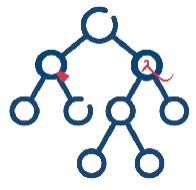
\includegraphics[height=1.0cm]{msca_logo.png}}%
    \end{center}

    \vspace{0.6cm}

    % Main title with Q logos on sides (with clickable links)
    \begin{center}
        \begin{minipage}{0.1\textwidth}
            \centering
            \href{https://quantlet.com}{
\includegraphics[height=1.1cm]{ql_logo.png}}
        \end{minipage}%
        \begin{minipage}{0.78\textwidth}
            \centering
            {\LARGE\bfseries\usebeamercolor[fg]{title}\inserttitle}

            \vspace{0.3cm}

            {\usebeamerfont{subtitle}\usebeamercolor[fg]{title}\insertsubtitle}
        \end{minipage}%
        \begin{minipage}{0.1\textwidth}
            \centering
            \href{https://quantinar.com}{
\includegraphics[height=1.1cm]{qr_logo.png}}
        \end{minipage}
    \end{center}

    \vspace{0.6cm}

    % Authors (left aligned)
    \hspace{0.5cm}{\usebeamerfont{author}\insertauthor}

    \vspace{0.3cm}

    % Institute/Affiliations (left aligned)
    \hspace{0.5cm}\begin{minipage}[t]{0.9\textwidth}
        \raggedright\small\insertinstitute
    \end{minipage}
}

%=============================================================================
% THEOREM ENVIRONMENTS
%=============================================================================
\theoremstyle{definition}
\setbeamertemplate{theorems}[numbered]
\ifdefined\sfmlang
\newtheorem{defn}{Definiție}
\newtheorem{thm}{Teoremă}
\newtheorem{prop}{Propoziție}
\newtheorem{rmk}{Observație}
\else
\newtheorem{defn}{Definition}
\newtheorem{thm}{Theorem}
\newtheorem{prop}{Proposition}
\newtheorem{rmk}{Remark}
\fi

%=============================================================================
% CENTRED MINIPAGE (no extra vertical space)
%=============================================================================
\newenvironment{cminipage}[1]{%
    \par\noindent\hfill\begin{minipage}{#1}\ignorespaces
}{%
    \end{minipage}\hfill\null\par
}

%=============================================================================
% CUSTOM COMMANDS
%=============================================================================
\newcommand{\E}{\mathbb{E}}
\newcommand{\Var}{\text{Var}}
\newcommand{\Cov}{\text{Cov}}
\newcommand{\Corr}{\text{Corr}}
\newcommand{\R}{\mathbb{R}}
\newcommand{\N}{\mathbb{N}}
\newcommand{\Z}{\mathbb{Z}}
\newcommand{\B}{\mathbf{B}}
\newcommand{\imark}{\textcolor{MainBlue}{\textbullet}}
\newcommand{\RMSE}{\text{RMSE}}
\newcommand{\MAE}{\text{MAE}}
\newcommand{\MAPE}{\text{MAPE}}



\newcommand{\qlurl}[1]{https://github.com/danpele/SFM/tree/main/Quantlets/Ch_14/#1}

% Clickable citations (DOIs verified via Crossref)

\newcommand{\refNakamoto}{\href{https://bitcoin.org/bitcoin.pdf}{Nakamoto (2008)}}
\newcommand{\refButerin}{\href{https://ethereum.org/en/whitepaper/}{Buterin (2014)}}
\newcommand{\refMerge}{\href{https://ethereum.org/en/roadmap/merge/}{ethereum.org: The Merge}}
\newcommand{\refLT}{\href{https://doi.org/10.1093/rfs/hhaa113}{Liu \& Tsyvinski (2021)}}
\newcommand{\refLTW}{\href{https://doi.org/10.1111/jofi.13119}{Liu, Tsyvinski \& Wu (2022)}}
\newcommand{\refGS}{\href{https://doi.org/10.1111/jofi.12903}{Griffin \& Shams (2020)}}
\newcommand{\refMS}{\href{https://doi.org/10.1016/j.jfineco.2019.07.001}{Makarov \& Schoar (2020)}}
\newcommand{\refGorton}{\href{https://doi.org/10.3386/w30796}{Gorton et al.\ (2022)}}
\newcommand{\refGZ}{\href{https://doi.org/10.2139/ssrn.3888752}{Gorton \& Zhang (2021)}}
\newcommand{\refLVN}{\href{https://doi.org/10.1016/j.jimonfin.2022.102777}{Lyons \& Viswanath-Natraj (2023)}}
\newcommand{\refLMS}{\href{https://doi.org/10.3386/w31160}{Liu, Makarov \& Schoar (2023)}}
\newcommand{\refMZZ}{\href{https://doi.org/10.3386/w33882}{Ma, Zeng \& Zhang (2025)}}
\newcommand{\refUrquhart}{\href{https://doi.org/10.1016/j.econlet.2016.09.019}{Urquhart (2016)}}
\newcommand{\refNC}{\href{https://doi.org/10.1016/j.econlet.2016.10.033}{Nadarajah \& Chu (2017)}}
\newcommand{\refTL}{\href{https://doi.org/10.1016/j.frl.2019.101382}{Tran \& Leirvik (2020)}}
\newcommand{\refCF}{\href{https://doi.org/10.1016/j.econlet.2015.02.029}{Cheah \& Fry (2015)}}
\newcommand{\refKatsiampa}{\href{https://doi.org/10.1016/j.econlet.2017.06.023}{Katsiampa (2017)}}
\newcommand{\refBL}{\href{https://doi.org/10.1111/j.1540-6288.2010.00244.x}{Baur \& Lucey (2010)}}
\newcommand{\refBHL}{\href{https://doi.org/10.1016/j.intfin.2017.12.004}{Baur, Hong \& Lee (2018)}}
\newcommand{\refCP}{\href{https://doi.org/10.1016/j.frl.2018.11.012}{Caporale \& Plastun (2019)}}
\newcommand{\refGHMO}{\href{https://doi.org/10.1016/j.jmoneco.2017.12.004}{Gandal et al.\ (2018)}}
\newcommand{\refHill}{\href{https://doi.org/10.1214/aos/1176343247}{Hill (1975)}}
\newcommand{\refBoll}{\href{https://doi.org/10.1016/0304-4076(86)90063-1}{Bollerslev (1986)}}
\newcommand{\refLM}{\href{https://doi.org/10.1093/rfs/1.1.41}{Lo \& MacKinlay (1988)}}
\newcommand{\refFama}{\href{https://doi.org/10.2307/2325486}{Fama (1970)}}
\newcommand{\refJLS}{\href{https://doi.org/10.1142/S0219024900000115}{Johansen, Ledoit \& Sornette (2000)}}
\newcommand{\refTH}{\href{https://doi.org/10.1016/j.jempfin.2018.08.004}{Trimborn \& Härdle (2018)}}
\newcommand{\refHHR}{\href{https://doi.org/10.1093/jjfinec/nbz033}{Härdle, Harvey \& Reule (2020)}}
\newcommand{\refFHH}{\href{https://doi.org/10.1007/978-3-030-13751-9}{Franke, Härdle \& Hafner (2019)}}
\newcommand{\refKupiec}{\href{https://doi.org/10.3905/jod.1995.407942}{Kupiec (1995)}}
\newcommand{\refWang}{\href{https://doi.org/10.1038/s41586-023-06221-2}{Wang et al.\ (2023)}}
\newcommand{\refPeleA}{\href{https://doi.org/10.1080/1351847X.2021.1960403}{Pele et al.\ (2023)}}
\newcommand{\refPeleB}{\href{https://doi.org/10.3390/e21020102}{Pele \& Mazurencu-Marinescu-Pele (2019)}}
\newcommand{\refMiCA}{\href{https://eur-lex.europa.eu/eli/reg/2023/1114/oj}{Regulamentul (EU) 2023/1114 (MiCA)}}
\newcommand{\refESMA}{\href{https://www.esma.europa.eu/esmas-activities/digital-finance-and-innovation/markets-crypto-assets-regulation-mica}{ESMA: MiCA}}
\newcommand{\refGENIUS}{\href{https://www.govinfo.gov/app/details/PLAW-119publ27}{GENIUS Act, Public Law 119-27}}
\newcommand{\refSEC}{\href{https://www.sec.gov/newsroom/speeches-statements/gensler-statement-spot-bitcoin-011023}{SEC (2024)}}
\newcommand{\refFed}{\href{https://www.federalreserve.gov/newsevents/pressreleases/monetary20230312b.htm}{Trezoreria SUA, Rezerva Federală și FDIC (2023)}}
\newcommand{\refFDIC}{\href{https://www.fdic.gov/news/press-releases/2023/pr23016.html}{FDIC (2023)}}
\newcommand{\refDL}{\href{https://api-docs.defillama.com/}{DefiLlama}}

\title[Statistica piețelor financiare]{Statistica piețelor financiare}
\subtitle{Capitolul 14: Active cripto}
\author[D.T. Pele]{Daniel Traian PELE}
\institute{Academia de Studii Economice din București\\
IDA Institute Digital Assets\\
Blockchain Research Center\\
AI4EFin Artificial Intelligence for Energy Finance\\
Academia Română, Institutul de Prognoză Economică\\
MSCA Digital Finance}
\date{}

%=============================================================================
\providecommand{\sfmapplink}[3]{\hypertarget{#2}{}\hyperlink{#1}{\beamergotobutton{#3}}}  % APPLINKS-MACROS
\providecommand{\sfmappback}[2]{\begin{tikzpicture}[remember picture,overlay]\node[anchor=south east] at ([xshift=-3mm,yshift=7mm]current page.south east){\hyperlink{#1}{\beamerreturnbutton{#2}}};\end{tikzpicture}}  % APPLINKS-MACROS
\providecommand{\sfmchlink}[2]{\href{#1}{#2}}  % APPLINKS-MACROS
\providecommand{\sfmchlinkt}[2]{\href{#1}{\usebeamercolor[fg]{frametitle}#2}}  % APPLINKS-MACROS
\begin{document}
%=============================================================================

{
\setbeamertemplate{headline}{}
\setbeamertemplate{footline}{}
\begin{frame}[noframenumbering]
    \titlepage
\end{frame}
}
% BEGIN-ACRONYMS (generat de latex/acronyms.py; nu editati manual)
\begin{frame}{Acronime folosite în acest material (1/2)}
\setbeamertemplate{itemize/enumerate body begin}{\tiny}
\begin{columns}[T]
\begin{column}{0.49\textwidth}
\begin{itemize}\setlength{\itemsep}{0pt}
    \item \textbf{ACF}: Autocorrelation Function (funcția de autocorelație)
    \item \textbf{AI}: Artificial Intelligence (inteligență artificială)
    \item \textbf{AIC}: Akaike Information Criterion (criteriul informațional Akaike)
    \item \textbf{API}: Application Programming Interface (interfață de programare a aplicațiilor)
    \item \textbf{AR}: AutoRegressive (model); in event studies: Abnormal Return (model autoregresiv; în studiile de eveniment: randament anormal)
    \item \textbf{CI}: Confidence Interval (interval de încredere)
    \item \textbf{COVID-19}: COronaVIrus Disease 2019 (boala provocată de coronavirus, 2019)
    \item \textbf{CRIX}: CRypto IndeX (indicele pieței cripto)
    \item \textbf{DAI}: Dai (stablecoin of the MakerDAO protocol) — stablecoin garantat cu active cripto, al protocolului MakerDAO
    \item \textbf{EODHD}: EOD Historical Data (market-data provider) — furnizor de date de piață
    \item \textbf{ES}: Expected Shortfall (pierderea așteptată în coadă)
    \item \textbf{ETF}: Exchange-Traded Fund (fond tranzacționat la bursă)
    \item \textbf{EWMA}: Exponentially Weighted Moving Average (medie mobilă ponderată exponențial)
\end{itemize}
\end{column}
\begin{column}{0.49\textwidth}
\begin{itemize}\setlength{\itemsep}{0pt}
    \item \textbf{FTX}: FTX Trading Ltd. (crypto exchange, bankrupt in November 2022) — bursa cripto FTX, falimentară în noiembrie 2022
    \item \textbf{GARCH}: Generalised AutoRegressive Conditional Heteroskedasticity (heteroscedasticitate condiționată autoregresivă generalizată)
    \item \textbf{GENIUS}: Guiding and Establishing National Innovation for U.S. Stablecoins (Act) — legea americană privind stablecoins de plată
    \item \textbf{GJR}: Glosten–Jagannathan–Runkle (asymmetric GARCH) — modelul GARCH asimetric Glosten–Jagannathan–Runkle
    \item \textbf{HAC}: Heteroskedasticity and Autocorrelation Consistent (standard errors) — erori standard robuste la heteroscedasticitate și autocorelație
    \item \textbf{HS}: Historical Simulation (simularea istorică)
    \item \textbf{IGARCH}: Integrated GARCH (GARCH integrat)
    \item \textbf{LPPL}: Log-Periodic Power Law (legea de putere log-periodică)
    \item \textbf{LUNA}: Luna (token of the Terra blockchain) — token-ul blockchain-ului Terra
    \item \textbf{SEC}: Securities and Exchange Commission (Comisia americană pentru valori mobiliare)
    \item \textbf{SHA-256}: Secure Hash Algorithm, 256 bits (algoritmul de hash securizat cu 256 de biți)
    \item \textbf{SUA}: Statele Unite ale Americii
    \item \textbf{SVB}: Silicon Valley Bank (banca Silicon Valley Bank)
\end{itemize}
\end{column}
\end{columns}
\end{frame}
\begin{frame}{Acronime folosite în acest material (2/2)}
\setbeamertemplate{itemize/enumerate body begin}{\tiny}
\begin{columns}[T]
\begin{column}{0.49\textwidth}
\begin{itemize}\setlength{\itemsep}{0pt}
    \item \textbf{USDC}: USD Coin (stablecoin garantat cu dolari, emis de Circle)
    \item \textbf{UST}: TerraUSD (stablecoin algoritmic al rețelei Terra)
    \item \textbf{UTC}: Coordinated Universal Time (Temps Universel Coordonné) — timpul universal coordonat
    \item \textbf{VR}: Variance Ratio (raportul varianțelor)
\end{itemize}
\end{column}
\begin{column}{0.49\textwidth}
\end{column}
\end{columns}
\end{frame}
% END-ACRONYMS

\begin{frame}{Întrebarea de azi și traseul}
\itemsize{\small}
\begin{itemize}
    \item \textbf{Întrebarea}: funcționează instrumentele statistice din \sfmchlink{https://danpele.github.io/SFM/RO/Cursuri/capitol2_distributii_clasice_fapte_stilizate.pdf}{Capitolele 2}--\sfmchlink{https://danpele.github.io/SFM/RO/Cursuri/capitol10_var_es_backtesting.pdf}{10} pe o piață care nu se închide niciodată, nu are fluxuri de numerar și poate pierde 80\% din valoare?
    \begin{itemize}
        \item răspunsul este o privire statistică asupra activelor cripto, nu un curs de criptografie
    \end{itemize}
    \item \textbf{Traseul} capitolului
    \begin{itemize}
        \item Bitcoin și Ethereum: blockchain, proof of work și proof of stake, halving-ul
        \item cripto ca o clasă de active: anualizarea cu 365 de zile, cozile, volatility clustering, GARCH, eficiența, weekendul
        \item corelația cu acțiunile și aurul; bulele și drawdown-urile; ETF-urile spot pe Bitcoin din 2024
        \item stablecoins: tipuri, ofertă, abateri de la paritate, USDC în martie 2023, prăbușirea TerraUSD; reglementarea; VaR 1\% și ES 2,5\%
    \end{itemize}
\end{itemize}
\end{frame}

\begin{frame}{Rezultatele învățării}
\itemsize{\small}
\begin{itemize}
    \item Explicați cum înregistrează un blockchain proprietatea, de ce mining-ul consumă energie și cum rezultă oferta de Bitcoin din regula halving-ului
    \item Anualizați randamentele și volatilitățile cripto cu frecvența reală (365 de zile) și explicați ce greșim cu 252
    \item Estimați indicele de coadă, un model GARCH(1,1)-t și testele raportului varianțelor pentru Bitcoin și comparați-le cu S\&P 500
    \item Măsurați în timp corelația activelor cripto cu acțiunile și aurul, precum și drawdown-urile unui activ cripto
    \item Descrieți cele trei tipuri de stablecoins, măsurați abaterea de la paritate în puncte de bază și interpretați un episod de depeg
    \item Calculați VaR 1\% și ES 2,5\% ale unei poziții cripto și verificați-le prin backtesting
\end{itemize}
\end{frame}

\begin{frame}{Bibliografie și instrumente}
\itemsize{\small}
\begin{itemize}
    \item Manual: \refFHH, cap.~23 (criptomonede)
    \begin{itemize}
        \item sinteze: \refHHR; indicele cripto CRIX: \refTH
        \item riscuri și randamente: \refLT; stablecoins: \refGorton, \refLVN
    \end{itemize}
    \item Quantlet-urile Python ale capitolului: \href{https://github.com/danpele/SFM/tree/main/Quantlets/Ch_14}{Quantlets/Ch\_14}
    \begin{itemize}
        \item date zilnice de la EODHD (închiderea cripto, 7 zile pe săptămînă); oferta de stablecoins de la \refDL
    \end{itemize}
    \item Notebook-ul cursului: \href{\colaburl{notebooks/EN/chapter14_lecture_notebook.ipynb}}{deschideți în Google Colab}
    \item Cursuri video: \quantinar{Introduction to Blockchain and Cryptocurrencies}{https://quantinar.com/course/134/introduction-to-blockchain-and-cryptocurrencies}; \quantinar{Cryptocurrency as an Asset Class}{https://quantinar.com/course/55/cryptoasset}
\end{itemize}
\end{frame}


%=============================================================================
\section{Bitcoin și Ethereum pe scurt}
%=============================================================================

\begin{frame}{De la o lucrare de nouă pagini la o piață}
\itemsize{\footnotesize}
\begin{columns}[T]
\begin{column}{0.62\textwidth}
\begin{itemize}
    \item 31 octombrie 2008: \refNakamoto{} propune „un sistem de numerar electronic peer-to-peer”
    \begin{itemize}
        \item \textbf{peer-to-peer}: utilizatorii își plătesc direct unii altora, fără o bancă la mijloc
        \item problema rezolvată: \textbf{dubla cheltuire} (double spending), adică plata de două ori cu aceeași monedă digitală
    \end{itemize}
    \item 3 ianuarie 2009: primul bloc; 2010: primele tranzacții pe exchange-uri
    \begin{itemize}
        \item \textbf{exchange}: o platformă de tranzacționare unde activele cripto se cumpără și se vînd contra dolari sau alte active cripto
    \end{itemize}
    \item \textbf{Activ cripto}: un activ digital a cărui proprietate este înregistrată într-un blockchain
    \begin{itemize}
        \item autorul, „Satoshi Nakamoto”, este încă necunoscut; monedele obținute prin mining în 2009--2010 nu au fost mutate niciodată
    \end{itemize}
\end{itemize}
\end{column}
\begin{column}{0.35\textwidth}
\centering
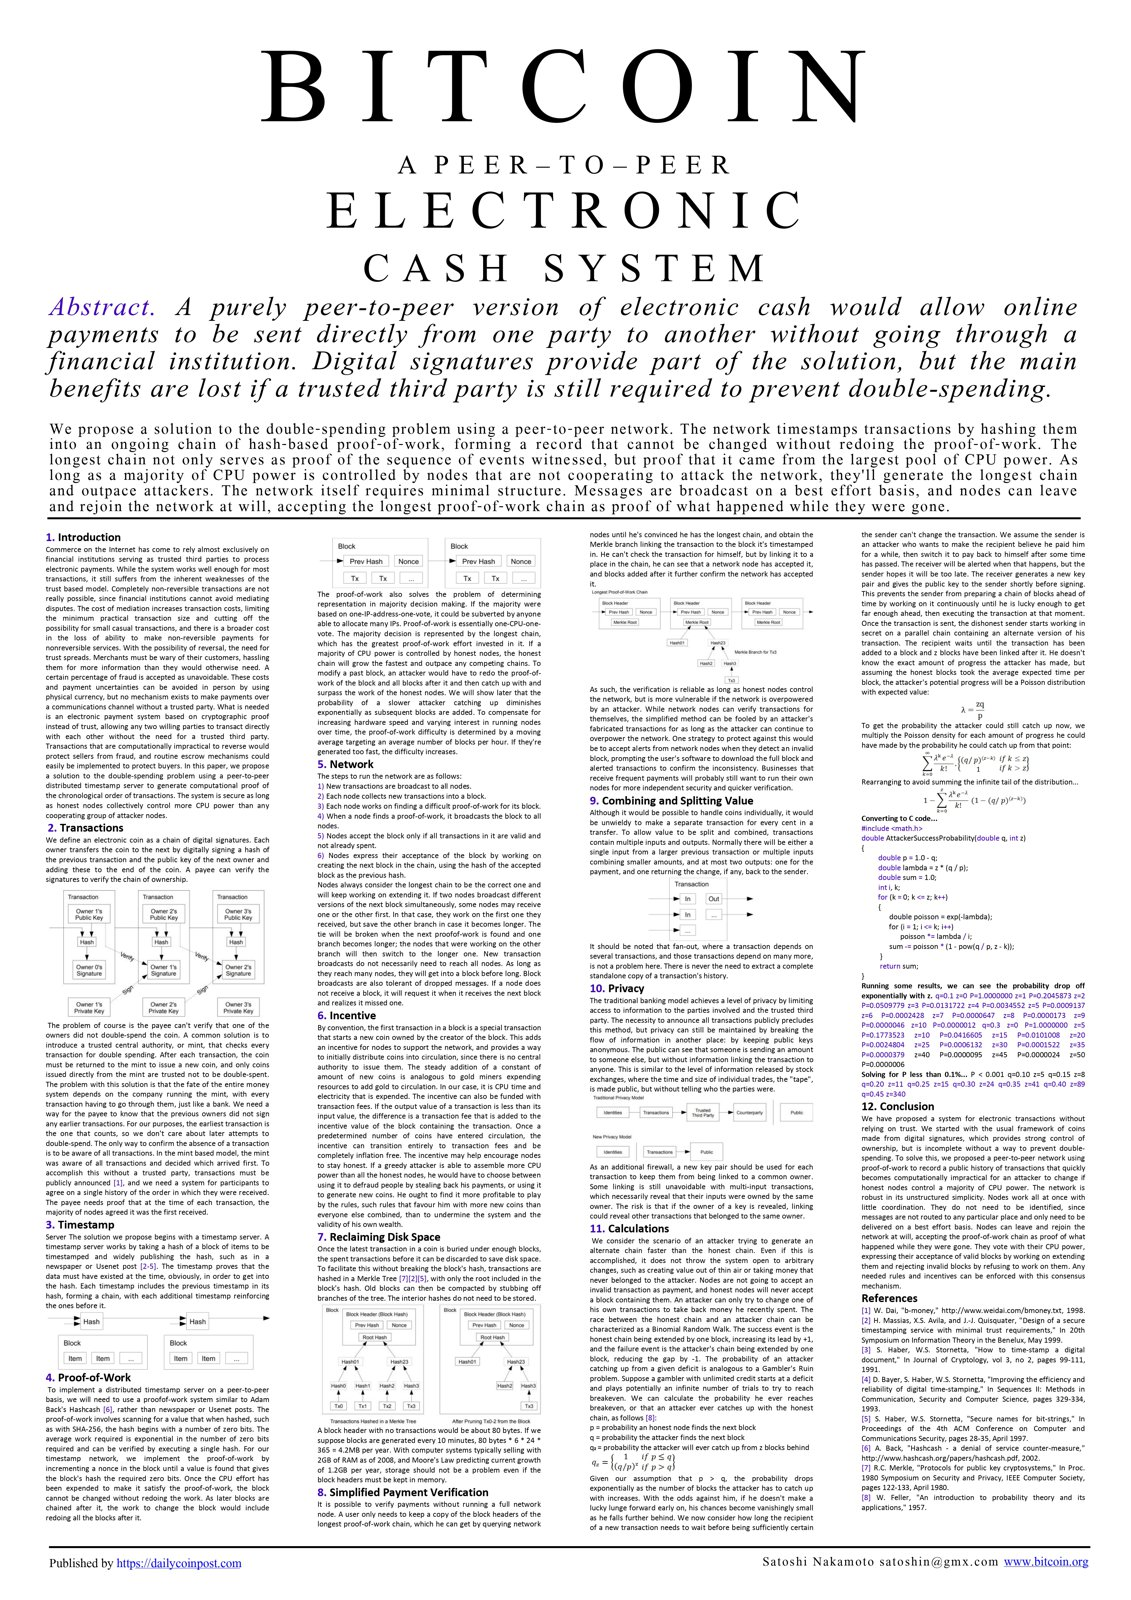
\includegraphics[height=0.50\textheight]{ch0_bitcoin_whitepaper.jpg}\\[1mm]
\imgcap{Lucrarea care a lansat Bitcoin, 2008}
\imgcredit{https://commons.wikimedia.org/wiki/File:Bitcoin-whitepaper-poster_page-0001.jpg}{Text: Satoshi Nakamoto (2008); afiș: DailyCoinPost (2018); CC0; Wikimedia Commons}
\end{column}
\end{columns}
\end{frame}

\begin{frame}{Blockchain-ul: un registru public}
\itemsize{\small}
\begin{itemize}
    \item \textbf{Registru} (ledger): lista tuturor tranzacțiilor; cine ține registrul știe cine ce deține
    \begin{itemize}
        \item băncile țin registre private; Bitcoin ține un singur registru public, copiat pe mii de calculatoare (\textbf{noduri})
    \end{itemize}
    \item \textbf{Bloc}: un pachet de tranzacții; \textbf{hash}: o amprentă scurtă a unui bloc (funcția SHA-256)
    \begin{itemize}
        \item schimbarea unui singur caracter dintr-un bloc îi schimbă complet hash-ul
        \item fiecare bloc conține hash-ul blocului anterior: blocurile formează un \textbf{lanț}
    \end{itemize}
    \item Consecința: rescrierea unei tranzacții vechi înseamnă rescrierea tuturor blocurilor ulterioare
    \begin{itemize}
        \item cine poate adăuga următorul bloc și cu ce cost decide regula de \textbf{consens} (slide-ul următor)
    \end{itemize}
    \item Proprietatea: o monedă aparține celui care deține cheia privată a adresei ei; o cheie pierdută înseamnă o monedă pierdută
\end{itemize}
\end{frame}

\begin{frame}{Proof of work și mining-ul}
\itemsize{\footnotesize}
\begin{columns}[T]
\begin{column}{0.58\textwidth}
\begin{itemize}
    \item \textbf{Proof of work} (PoW): pentru a adăuga un bloc, un \textbf{miner} trebuie să găsească un număr care face hash-ul blocului mai mic decît o țintă
    \begin{itemize}
        \item singura metodă este încercarea repetată: miliarde de hash-uri pe secundă, pe mașini specializate
        \item ținta se ajustează la fiecare 2016 blocuri, astfel încît un bloc să apară cam la 10 minute
    \end{itemize}
    \item Cîștigătorul primește \textbf{subvenția blocului} (monede noi) plus comisioanele tranzacțiilor
    \begin{itemize}
        \item pentru a rescrie istoria, un atacator ar avea nevoie de mai multă putere de calcul decît toți minerii onești la un loc
    \end{itemize}
    \item Costul securității este electricitatea: de aceea Bitcoin este criticat pentru consumul de energie
\end{itemize}
\end{column}
\begin{column}{0.39\textwidth}
\centering
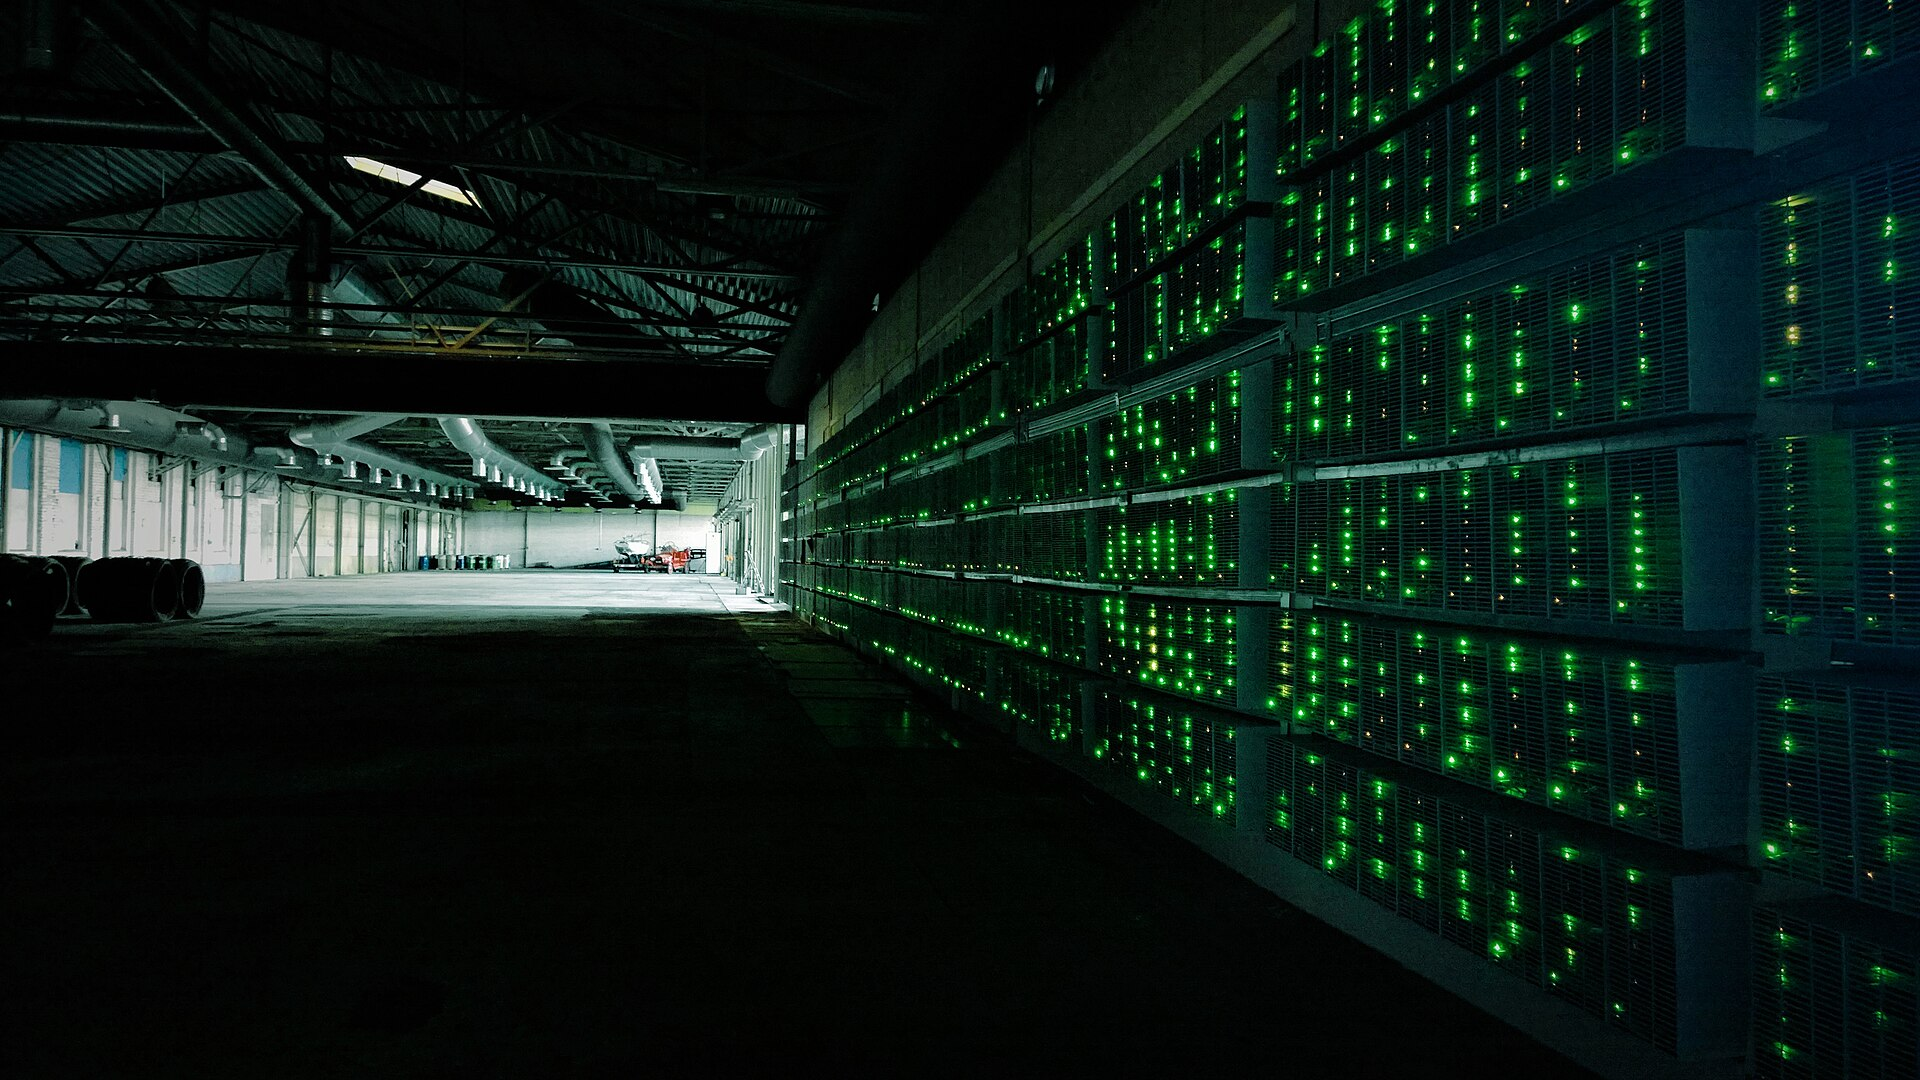
\includegraphics[height=0.36\textheight]{ch14_mining_farm_2014.jpg}\\[1mm]
\imgcap{O fermă de mining pentru Bitcoin, 2014}
\imgcredit{https://commons.wikimedia.org/wiki/File:Bitcoin_mining_farm.jpg}{Foto: Marko Ahtisaari (2014); CC BY 2.0; Wikimedia Commons}
\end{column}
\end{columns}
\end{frame}

\begin{frame}{Regula ofertei și halving-ul}
\itemsize{\small}
\begin{itemize}
    \item Subvenția blocului: 50 BTC din 2009, \textbf{înjumătățită} la fiecare 210\,000 de blocuri (cam patru ani)
    \begin{itemize}
        \item 2012: 25; 2016: 12,5; 2020: 6,25; aprilie 2024: 3,125 BTC pe bloc
        \item evenimentul înjumătățirii subvenției se numește \textbf{halving}
    \end{itemize}
    \item Oferta totală: o serie geometrică
    \begin{itemize}
        \item $210\,000 \times 50 \times (1 + \tfrac12 + \tfrac14 + \dots) = 210\,000 \times 50 \times 2 = 21$ de milioane de BTC
        \item circa 19{,}4 milioane la începutul lui 2024, 20{,}4 milioane în 2030: aproape toate monedele există deja
    \end{itemize}
    \item Datele halving-urilor se cunosc cu ani înainte
    \begin{itemize}
        \item pe o piață eficientă (\sfmchlink{https://danpele.github.io/SFM/RO/Cursuri/capitol7_piete_eficiente_mers_aleator_vr.pdf}{Capitolul 7}), o reducere previzibilă a ofertei noi ar trebui să fie deja inclusă în preț
    \end{itemize}
\end{itemize}
\end{frame}

\begin{frame}{Prețul și oferta de Bitcoin}
\itemsize{\footnotesize}
\begin{center}
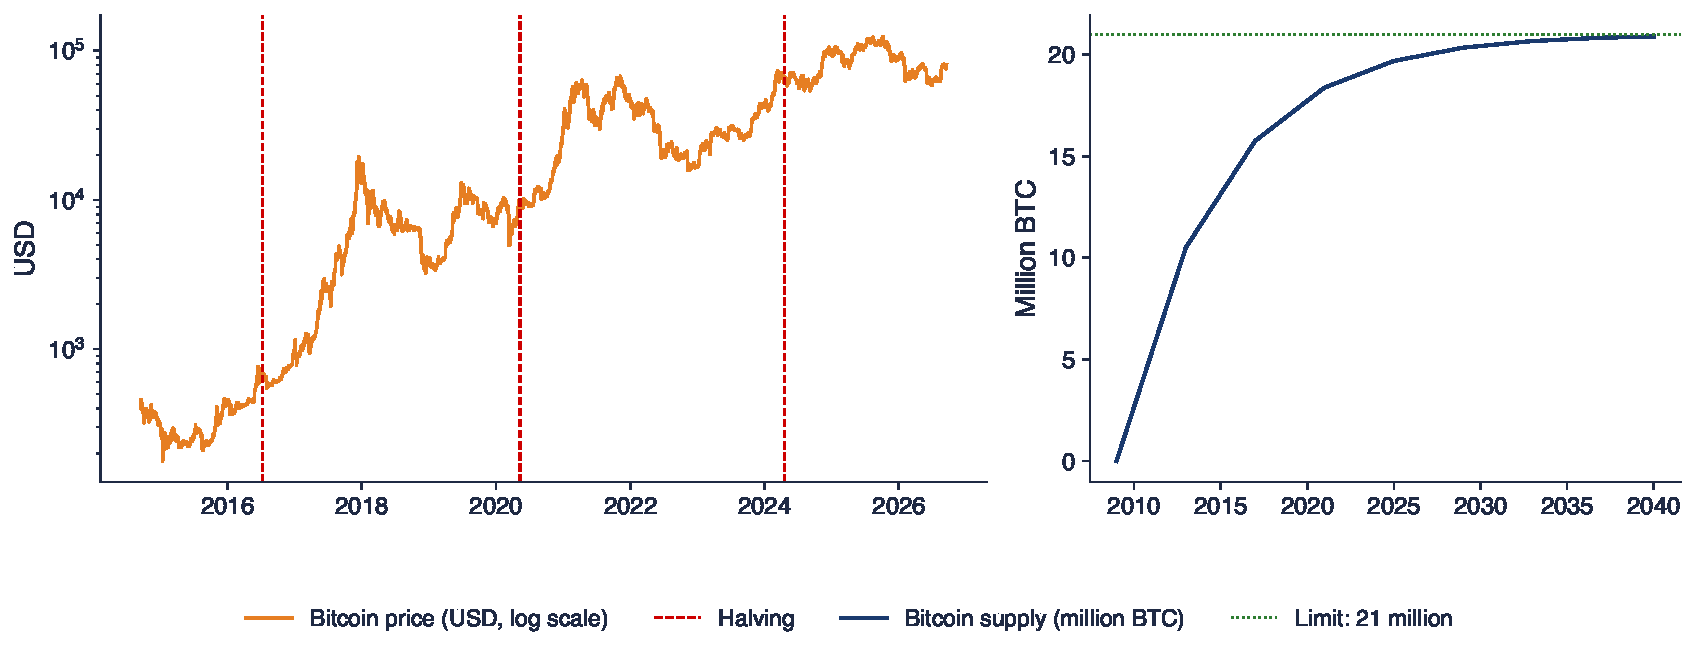
\includegraphics[width=0.97\textwidth,height=0.50\textheight,keepaspectratio]{sfm_ch14_halving.pdf}
\end{center}
\vspace{-0.25cm}
\begin{itemize}
    \item Stînga: închiderea Bitcoin în USD (scală logaritmică), 457 USD în septembrie 2014 și 80\,901 USD pe 18 septembrie 2026; linii întrerupte: halving-urile din 2016, 2020 și 2024. Dreapta: oferta din regula protocolului
    \item Interpretare: la un an după halving-uri, prețul era mai mare cu 287\%, 559\% și 31\%; trei observații nu sînt o dovadă, iar efectul se micșorează
\end{itemize}
\sfmquantlet{Ch_14}{SFM_ch14_bitcoin_basics}
\end{frame}

\begin{frame}{Un fondator anonim}
\itemsize{\footnotesize}
\begin{columns}[T]
\begin{column}{0.62\textwidth}
\begin{itemize}
    \item Nimeni nu știe cine este „Satoshi Nakamoto”; fondatorul a încetat să mai scrie în 2011
    \begin{itemize}
        \item regulile Bitcoin se schimbă doar dacă majoritatea nodurilor acceptă noul software
    \end{itemize}
    \item Consecințe pentru un statistician
    \begin{itemize}
        \item nicio companie, niciun profit, niciun dividend: niciun flux de numerar de actualizat
        \item prețul reflectă doar cererea: plăți, speculație, încrederea în raritate \refBHL
        \item deci modelele obișnuite de evaluare nu se aplică; studiem prețul ca obiect statistic
    \end{itemize}
    \item Tranzacțiile au loc non-stop pe sute de exchange-uri, 365 de zile pe an
\end{itemize}
\end{column}
\begin{column}{0.35\textwidth}
\centering
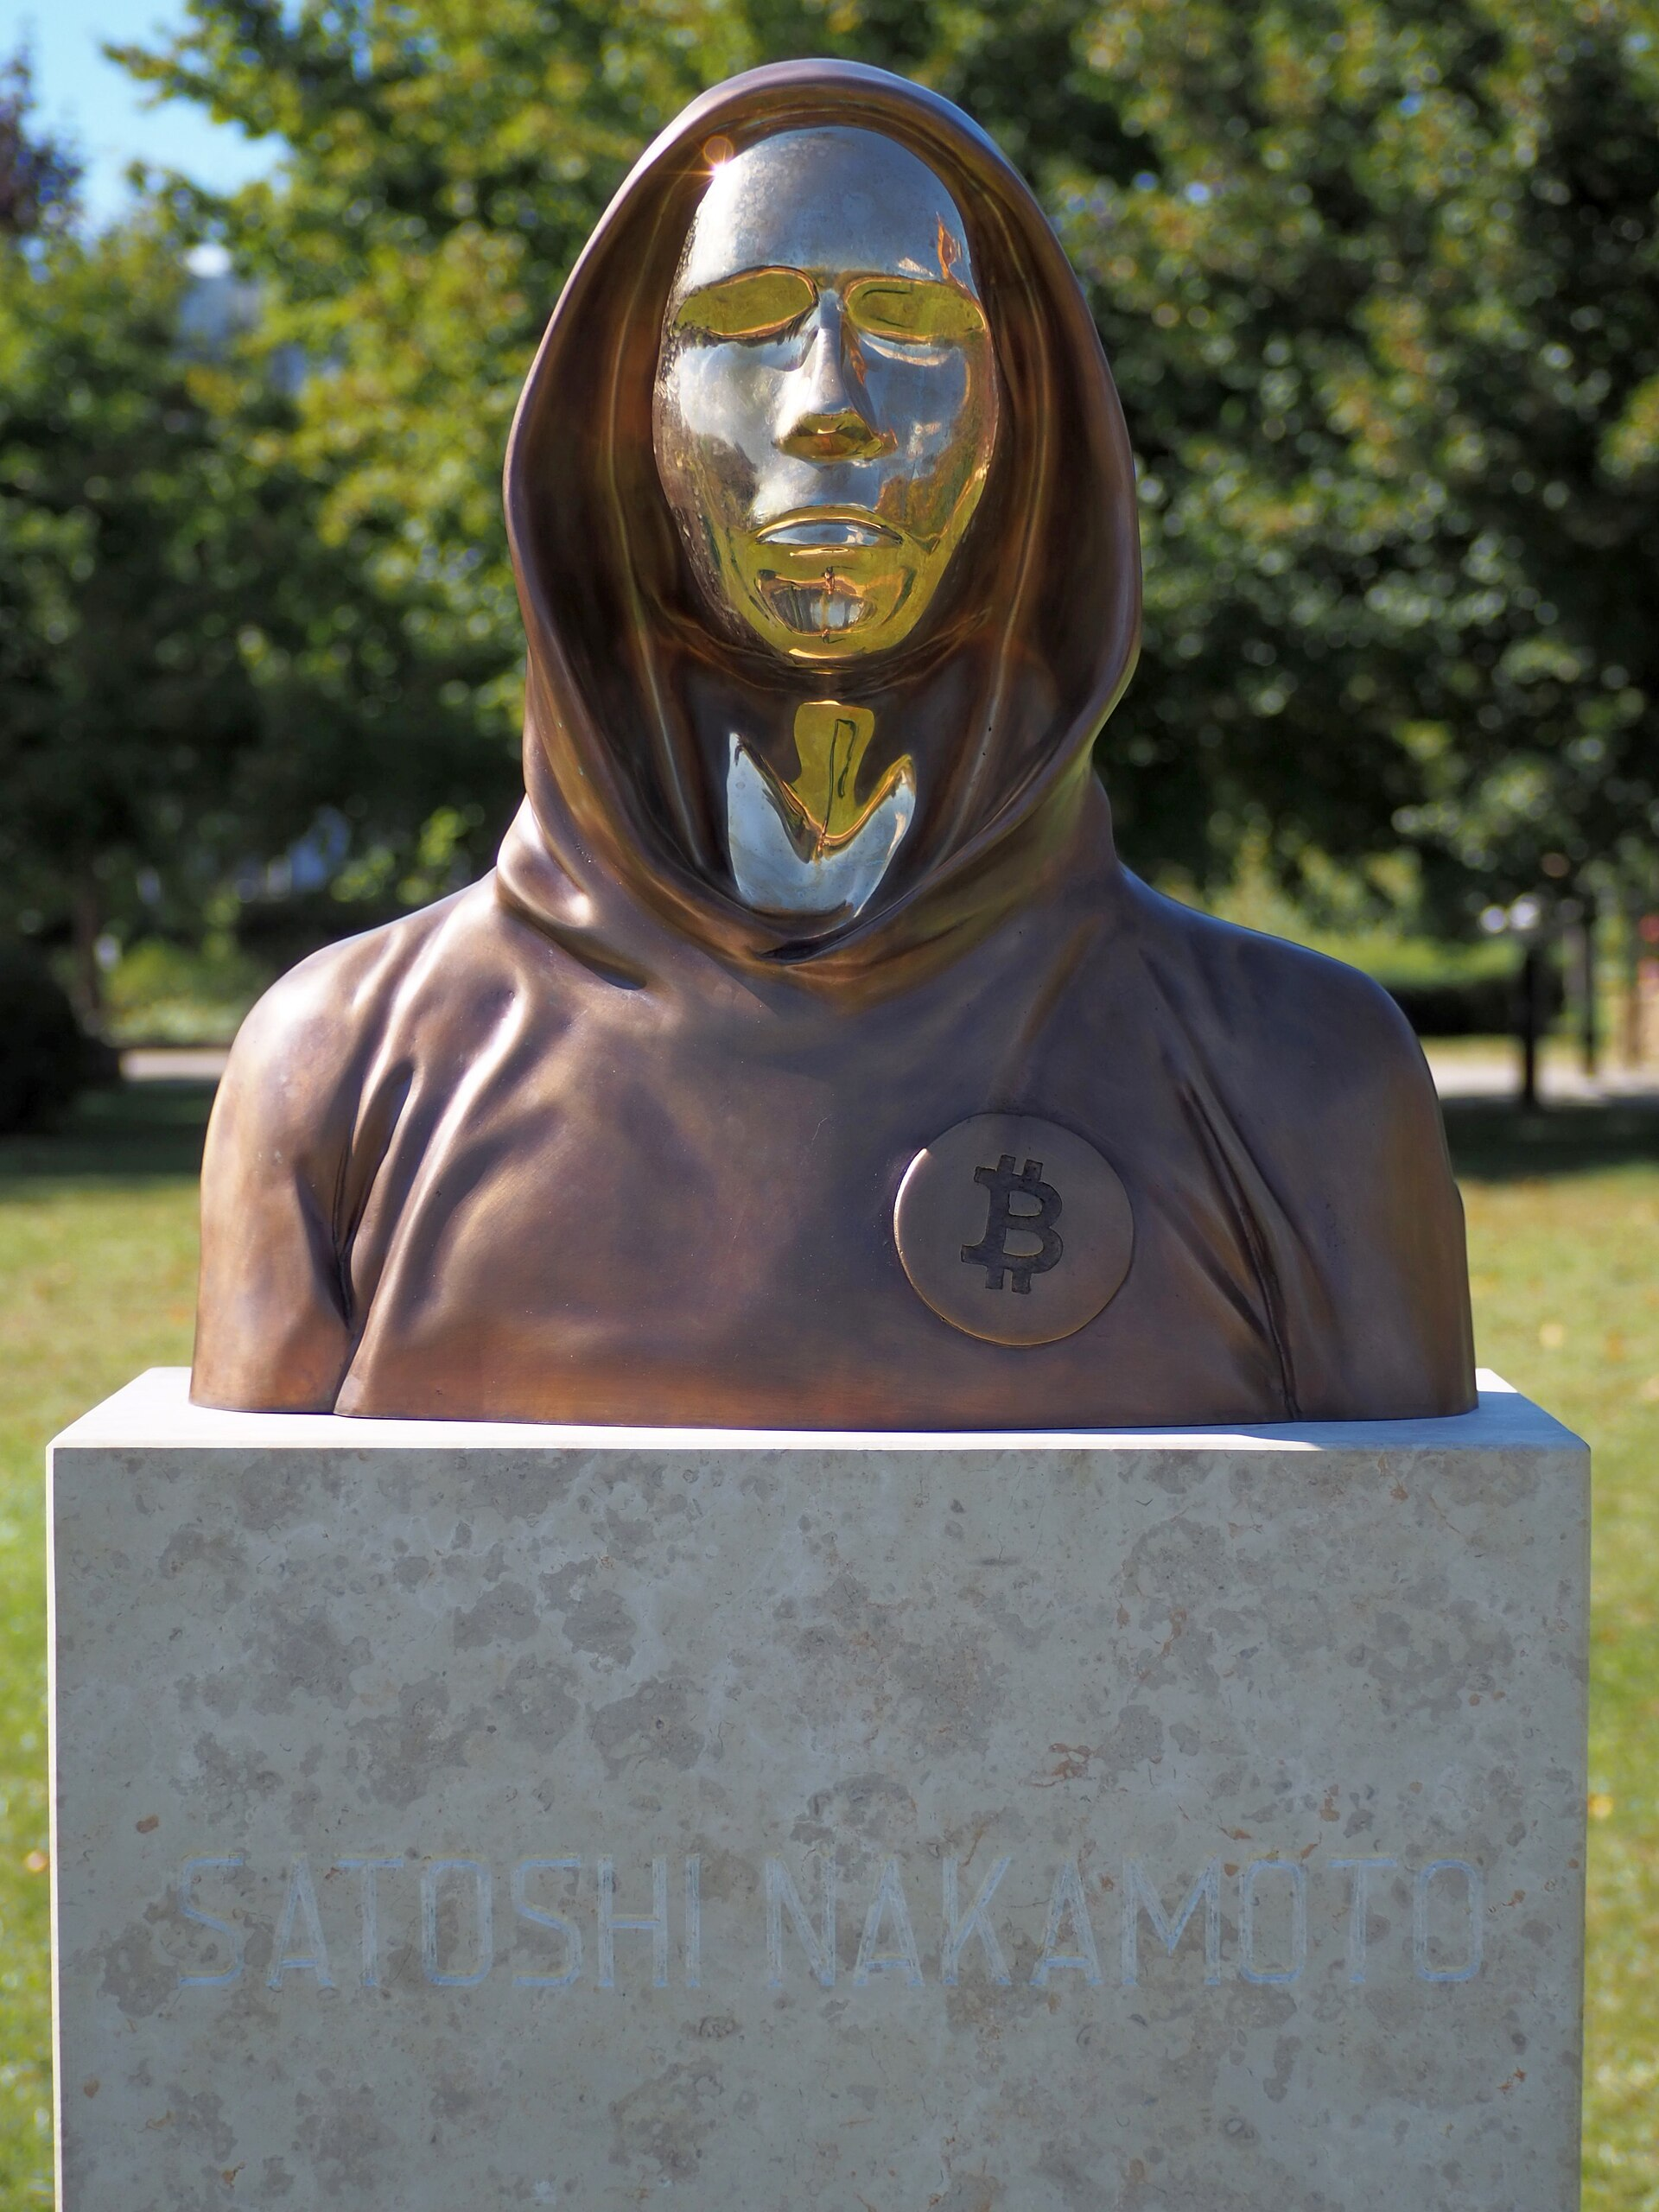
\includegraphics[height=0.46\textheight]{ch14_satoshi_bust_2021.jpg}\\[1mm]
\imgcap{Bustul lui Satoshi Nakamoto, Budapesta}
\imgcredit{https://commons.wikimedia.org/wiki/File:Bust_of_Satoshi_Nakamoto_in_Budapest.jpg}{Foto: Fekist (2021); CC BY-SA 4.0; Wikimedia Commons}
\end{column}
\end{columns}
\end{frame}

\begin{frame}{Ethereum, contractele inteligente și proof of stake}
\itemsize{\footnotesize}
\begin{columns}[T]
\begin{column}{0.64\textwidth}
\begin{itemize}
    \item 2014: \refButerin{} propune Ethereum, un blockchain care execută programe; lansat în iulie 2015
    \begin{itemize}
        \item \textbf{contract inteligent} (smart contract): un program stocat în blockchain care execută o tranzacție cînd condițiile lui sînt îndeplinite
        \item pe baza lui: token-uri, stablecoins și DeFi (finanțe descentralizate: credit și tranzacționare fără intermediari)
    \end{itemize}
    \item \textbf{Proof of stake} (PoS): dreptul de a adăuga un bloc se trage la sorți proporțional cu monedele blocate drept garanție (\textbf{stake})
    \begin{itemize}
        \item frauda se pedepsește prin pierderea garanției; nu mai există o cursă a puterii de calcul
        \item 15 septembrie 2022 („the Merge”): Ethereum trece de la PoW la PoS; consumul de energie scade cu peste 99,9\% \refMerge
    \end{itemize}
\end{itemize}
\end{column}
\begin{column}{0.33\textwidth}
\centering
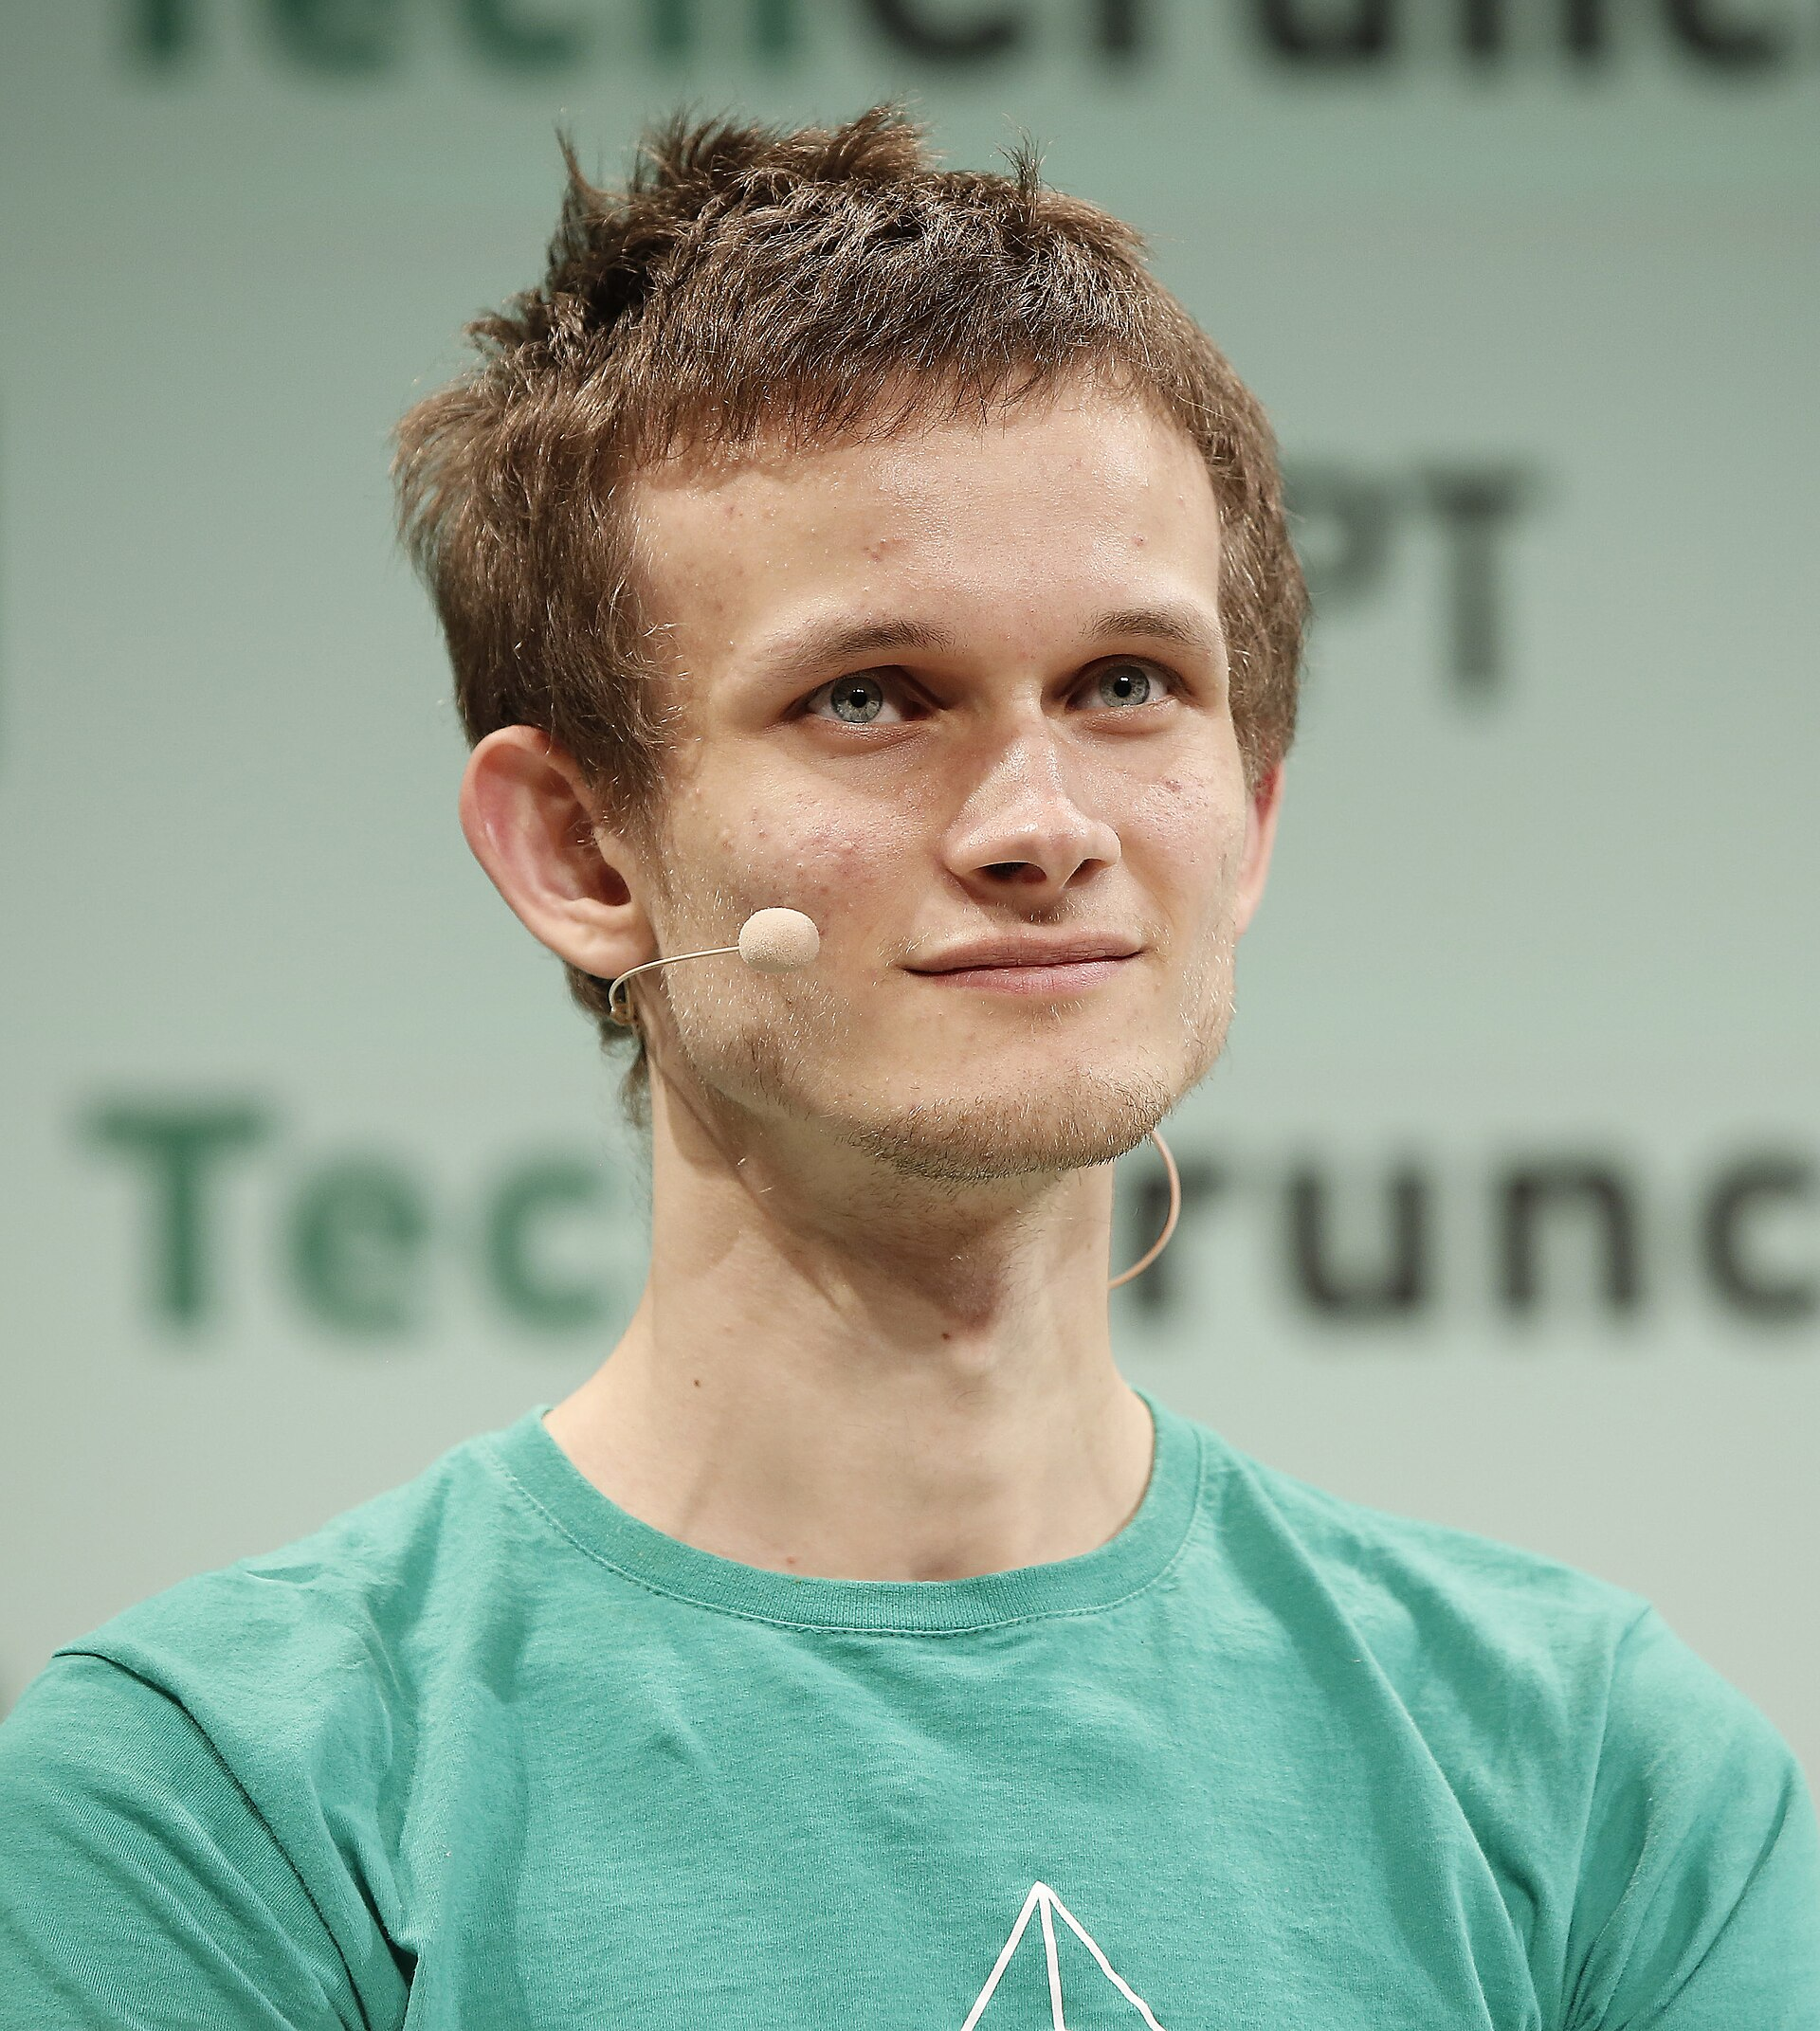
\includegraphics[height=0.42\textheight]{ch14_buterin_2015.jpg}\\[1mm]
\imgcap{Vitalik Buterin, 2015}
\imgcredit{https://commons.wikimedia.org/wiki/File:Vitalik_Buterin_TechCrunch_London_2015_(cropped).jpg}{Foto: John Phillips (2015); CC BY 2.0; Wikimedia Commons}
\end{column}
\end{columns}
\end{frame}

\begin{frame}{Prețuri și date}
\itemsize{\footnotesize}
\begin{columns}[T]
\begin{column}{0.64\textwidth}
\begin{itemize}
    \item Nu există un exchange unic: fiecare platformă are propriul preț; prețurile diferă între țări \refMS
    \begin{itemize}
        \item un furnizor de date agregă platformele într-o serie zilnică; aici: EODHD, închiderea la miezul nopții UTC (Coordinated Universal Time, ora universală coordonată)
    \end{itemize}
    \item Șapte zile de tranzacționare pe săptămînă: fără goluri de weekend, fără sărbători
    \begin{itemize}
        \item Bitcoin: 4\,384 de randamente zilnice din 2014; S\&P 500: 3\,017 de randamente în aceeași perioadă
    \end{itemize}
    \item Există indici de piață cu multe monede, de exemplu CRIX (Crypto Index) \refTH
    \begin{itemize}
        \item CRIX alege numărul de monede cu criteriul AIC (\sfmchlink{https://danpele.github.io/SFM/RO/Cursuri/capitol6_selectia_modelului_managementul_riscului.pdf}{Capitolul 6}): puține monede descriu întreaga piață
    \end{itemize}
    \item Randamentele: $r_t = 100(\ln P_t - \ln P_{t-1})$ în \%, fiecare serie pe propriul calendar
\end{itemize}
\end{column}
\begin{column}{0.33\textwidth}
\centering
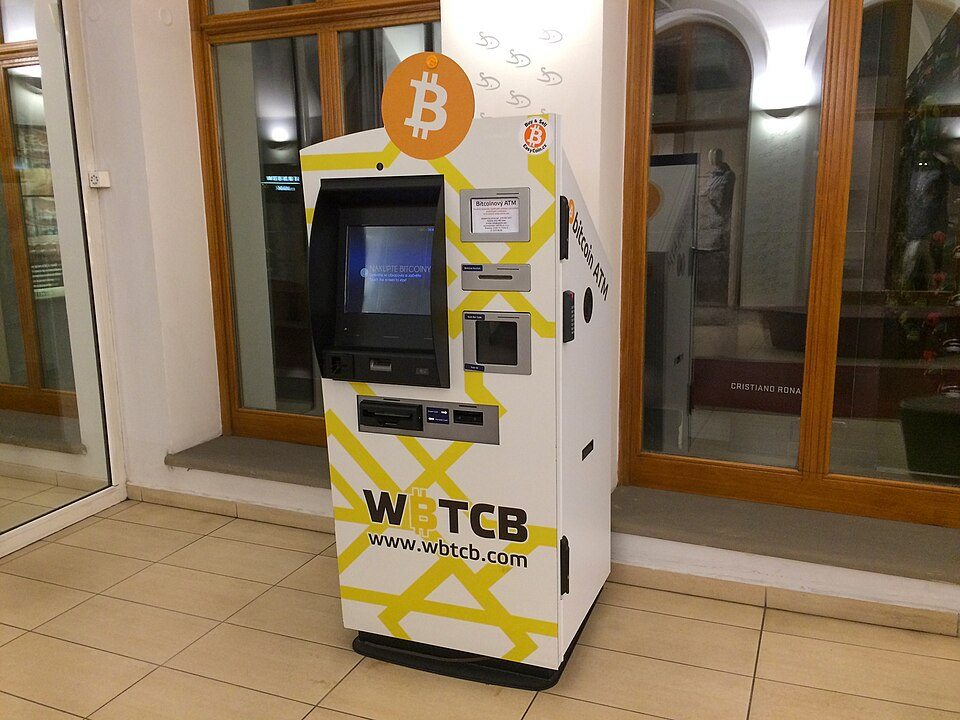
\includegraphics[height=0.40\textheight]{ch11_bitcoin_atm_prague.jpg}\\[1mm]
\imgcap{Un bancomat Bitcoin, Praga}
\imgcredit{https://commons.wikimedia.org/wiki/File:Bitcoin_ATM_Prague.jpg}{Foto: Perituss (2016); CC0; Wikimedia Commons}
\end{column}
\end{columns}
\end{frame}

\begin{frame}{Recapitulare: noțiuni de bază despre Bitcoin și Ethereum}
\itemsize{\small}
\begin{itemize}
    \item Un blockchain este un lanț public de blocuri legate prin hash-uri; schimbarea trecutului înseamnă refacerea întregii munci ulterioare
    \item PoW plătește minerii pentru calcul; PoS cere validatorilor o garanție; Ethereum a trecut la PoS în 2022
    \item Oferta de Bitcoin este fixată de regula halving-ului la 21 de milioane; nu există fluxuri de numerar, doar prețuri
\end{itemize}
\end{frame}


%=============================================================================
\section{Cripto ca o clasă de active}
%=============================================================================

\begin{frame}{Anualizarea cu frecvența reală}
\itemsize{\footnotesize}
\begin{itemize}
    \item Cu $m$ observații pe an și randamente zilnice i.i.d.: media anuală $= m\,\bar r$, volatilitatea anuală $= \sqrt{m}\,s$ (\sfmchlink{https://danpele.github.io/SFM/RO/Cursuri/capitol1_date_randamente_indicatori.pdf}{Capitolul 1})
    \begin{itemize}
        \item acțiunile: $m \approx 252$ de zile de tranzacționare; cripto: $m = 365$ (frecvența reală: $m = 365{,}3$ pentru Bitcoin, 251{,}4 pentru S\&P 500)
    \end{itemize}
    \item \textbf{Exemplu lucrat}: Bitcoin, $\bar r = 0{,}118\%$, $s = 3{,}49\%$ pe zi
    \begin{itemize}
        \item corect: $\sqrt{365} \times 3{,}49 = 19{,}10 \times 3{,}49 = 66{,}6\%$; media $365 \times 0{,}118 = 43{,}1\%$
        \item greșit: $\sqrt{252} \times 3{,}49 = 55{,}3\%$ și $252 \times 0{,}118 = 29{,}8\%$
    \end{itemize}
    \item Regula cu 252 subestimează volatilitatea cu 16{,}9\% și media cu 31{,}0\%
    \begin{itemize}
        \item amestecul lor (media $\times 252$, volatilitatea $\times\sqrt{365}$) deformează și raportul Sharpe
        \item comparațiile cu acțiunile: anualizăm fiecare serie cu propriul $m$, niciodată cu unul comun
    \end{itemize}
\end{itemize}
\end{frame}

\begin{frame}{Cinci active comparate}
\itemsize{\footnotesize}
\begin{center}
\scriptsize
\begin{tabular}{lrrrrrrrr}
\toprule
& din & $n$ & media (\%) & ab.\ std.\ (\%) & vol.\ anuală (\%) & asim. & exces boltire & min (\%) \\
\midrule
Bitcoin & 2014 & 4\,384 & $0{,}118$ & $3{,}49$ & $66{,}6$ & $-0{,}70$ & $12{,}0$ & $-46{,}5$ \\
Ethereum & 2016 & 3\,913 & $0{,}202$ & $4{,}99$ & $95{,}3$ & $-0{,}20$ & $9{,}0$ & $-55{,}1$ \\
Solana & 2020 & 2\,351 & $0{,}212$ & $6{,}12$ & $117{,}1$ & $-0{,}22$ & $7{,}9$ & $-55{,}0$ \\
S\&P 500 & 2014 & 3\,017 & $0{,}044$ & $1{,}11$ & $17{,}6$ & $-0{,}64$ & $15{,}8$ & $-12{,}8$ \\
Aur & 2014 & 3\,124 & $0{,}041$ & $1{,}01$ & $16{,}4$ & $-0{,}41$ & $9{,}5$ & $-11{,}1$ \\
\bottomrule
\end{tabular}
\end{center}
\begin{itemize}
    \item Randamente logaritmice zilnice pînă pe 18 septembrie 2026; volatilitatea anuală $= \sqrt{m}\,s$ cu frecvența reală $m$ a fiecărei serii; aurul: XAU/USD
    \item Interpretare
    \begin{itemize}
        \item Bitcoin este de 3{,}8 ori mai volatil decît S\&P 500 (66{,}6\% față de 17{,}6\%); Ethereum de 5{,}4 ori, Solana de 6{,}7 ori
        \item în 11{,}6\% din zile, Bitcoin se mișcă cu peste 5\%; cea mai proastă zi: $-46{,}5\%$ pe 12 martie 2020
        \item toate cinci au asimetrie negativă și exces de boltire: faptele stilizate din \sfmchlink{https://danpele.github.io/SFM/RO/Cursuri/capitol2_distributii_clasice_fapte_stilizate.pdf}{Capitolul 2} se păstrează, într-o formă mai puternică
    \end{itemize}
\end{itemize}
\end{frame}

\begin{frame}{Volatilitatea în timp}
\itemsize{\footnotesize}
\begin{center}
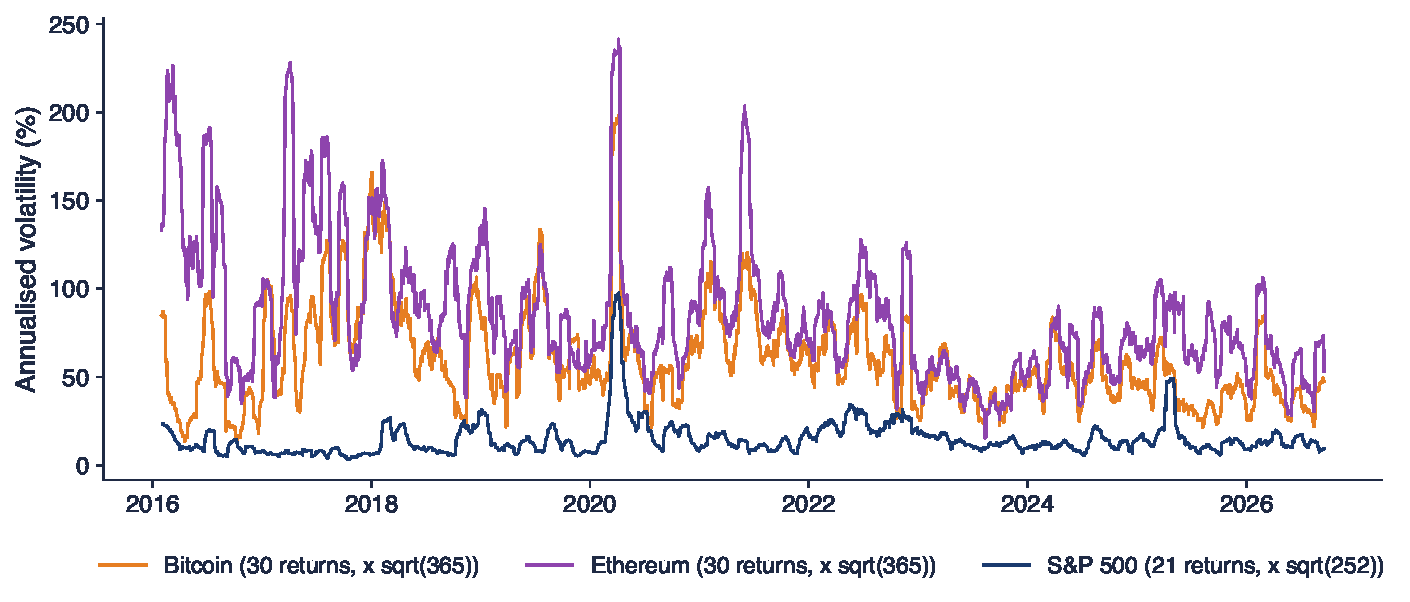
\includegraphics[width=0.97\textwidth,height=0.46\textheight,keepaspectratio]{sfm_ch14_rolling_vol.pdf}
\end{center}
\vspace{-0.25cm}
\begin{itemize}
    \item Volatilitatea pe circa o lună: 30 de randamente zilnice $\times\sqrt{365}$ pentru cripto, 21 de randamente $\times\sqrt{252}$ pentru S\&P 500
    \item Interpretare: medianele 54\% (Bitcoin), 77\% (Ethereum), 12\% (S\&P 500); raportul median Bitcoin/S\&P 500 este 3{,}8; toate trei ating maximul în martie--aprilie 2020
    \item Volatilitatea Bitcoin scade în timp, dar a fost sub cea a S\&P 500 doar în 0{,}1\% din zile
\end{itemize}
\sfmquantlet{Ch_14}{SFM_ch14_asset_class}
\end{frame}

\begin{frame}{Studiu de caz: riscurile și randamentele criptomonedelor}
\itemsize{\small}
\begin{itemize}
    \item \refLT: Bitcoin, Ripple și Ethereum, randamente zilnice și săptămînale, 2011--2018
    \begin{itemize}
        \item designul: regresia randamentelor cripto pe factorii pieței de acțiuni, pe valute, mărfuri și factori macroeconomici
    \end{itemize}
    \item Rezultatele
    \begin{itemize}
        \item randamentele cripto nu au aproape nicio expunere la factorii obișnuiți: o clasă de active separată
        \item momentum puternic în timp: randamentele mari dintr-o săptămînă prognozează randamente mari în săptămînile următoare
        \item atenția investitorilor (căutări Google, postări pe Twitter) prognozează randamentele
    \end{itemize}
    \item Continuare \refLTW: trei factori cripto (piața, dimensiunea, momentum) explică randamentele transversale ale monedelor
    \begin{itemize}
        \item legătura cu acțiunile s-a schimbat după 2020 (secțiunea 5): rezultatele depind de perioada eșantionului
    \end{itemize}
\end{itemize}
\end{frame}

\begin{frame}{Este weekendul diferit?}
\itemsize{\small}
\begin{itemize}
    \item Bursele de acțiuni se închid în weekend; piețele cripto nu, dar băncile, investitorii instituționali și știrile încetinesc
    \begin{itemize}
        \item \textbf{efectul zilei din săptămînă}: medie sau varianță diferită a randamentelor în anumite zile \refCP
    \end{itemize}
    \item Două teste pe Bitcoin, fiecare zi etichetată după data închiderii
    \begin{itemize}
        \item media: $r_t = a + b\,W_t + \varepsilon_t$, $W_t = 1$ sîmbăta și duminica; erori standard HAC (Newey--West)
        \item varianța: testul Brown--Forsythe (testul Levene în jurul medianei), robust la cozi groase
    \end{itemize}
    \item Raportul dintre varianța din weekend și cea din zilele lucrătoare: egal cu 1 dacă fiecare zi ar avea același risc
\end{itemize}
\end{frame}

\begin{frame}{Volatilitatea Bitcoin pe zile ale săptămînii}
\itemsize{\footnotesize}
\begin{center}
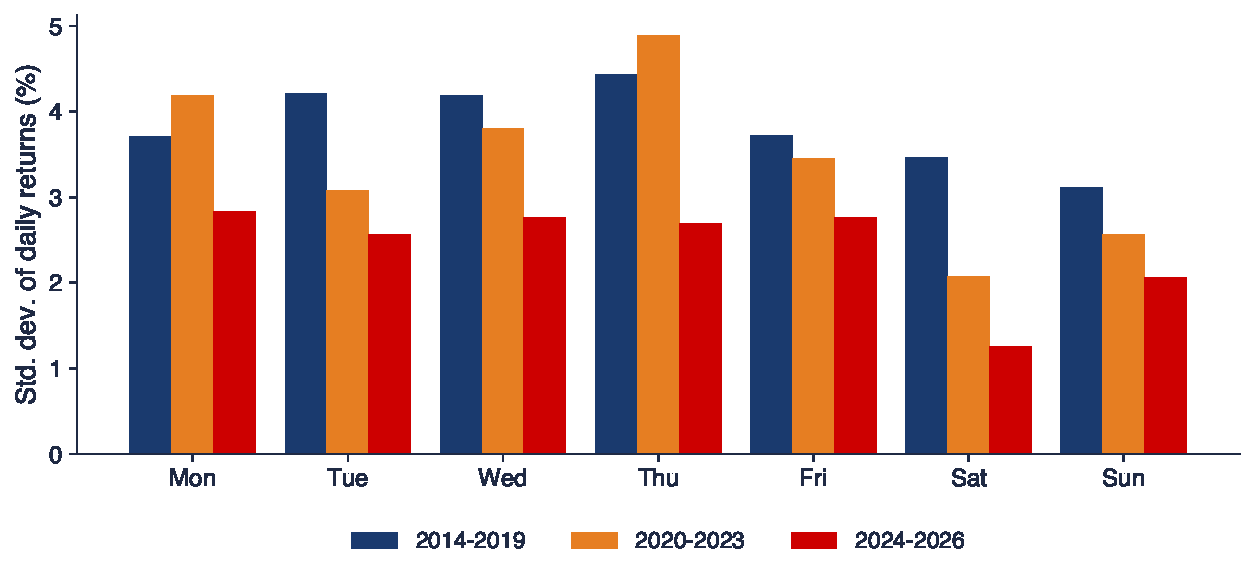
\includegraphics[width=0.97\textwidth,height=0.44\textheight,keepaspectratio]{sfm_ch14_weekday.pdf}
\end{center}
\vspace{-0.25cm}
\begin{itemize}
    \item Abaterea standard a randamentelor zilnice după ziua închiderii; trei perioade
    \item Variabila weekend $b$ (p-valoarea): $-0{,}01$ (0{,}95); $-0{,}11$ (0{,}48); $-0{,}03$ (0{,}83): niciun efect de weekend în medie
    \item Interpretare: varianța weekend/zile lucrătoare 0{,}66; 0{,}35; 0{,}39 (Brown--Forsythe p 0{,}002; $<$\,0{,}001; $<$\,0{,}001): piața cripto este mai liniștită cînd piețele tradiționale sînt închise
\end{itemize}
\sfmquantlet{Ch_14}{SFM_ch14_asset_class}
\end{frame}

\begin{frame}{Recapitulare: cripto ca o clasă de active}
\itemsize{\small}
\begin{itemize}
    \item Anualizăm cripto cu 365 de zile: Bitcoin 66{,}6\% pe an, nu 55{,}3\%
    \item Volatilitatea cripto este de 3{,}8 (Bitcoin) pînă la 6{,}7 (Solana) ori cea a S\&P 500 și este în scădere
    \item Niciun efect de weekend în medie, un efect puternic în varianță
\end{itemize}
\end{frame}


%=============================================================================
\section{Cozi și volatility clustering}
%=============================================================================

\begin{frame}{Cozi groase: estimatorul Hill}
\itemsize{\footnotesize}
\begin{center}
\scriptsize
\begin{tabular}{lrrrr}
\toprule
& coada stîngă $\hat\alpha$ & CI 95\% & coada dreaptă $\hat\alpha$ & CI 95\% \\
\midrule
Bitcoin & $2{,}71$ & $[2{,}20; 3{,}21]$ & $3{,}37$ & $[2{,}74; 4{,}00]$ \\
Ethereum & $2{,}62$ & $[2{,}10; 3{,}15]$ & $3{,}09$ & $[2{,}48; 3{,}71]$ \\
Solana & $2{,}84$ & $[2{,}11; 3{,}57]$ & $3{,}41$ & $[2{,}54; 4{,}29]$ \\
S\&P 500 & $2{,}68$ & $[2{,}08; 3{,}29]$ & $2{,}80$ & $[2{,}17; 3{,}43]$ \\
Aur & $3{,}11$ & $[2{,}42; 3{,}80]$ & $3{,}04$ & $[2{,}36; 3{,}71]$ \\
\bottomrule
\end{tabular}
\end{center}
\begin{itemize}
    \item \refHill{} (\sfmchlink{https://danpele.github.io/SFM/RO/Cursuri/capitol5_cozi_groase_evt.pdf}{Capitolul 5}): $\hat\alpha = \big[\frac1k\sum_{i=1}^k \ln(X_{(i)}/X_{(k+1)})\big]^{-1}$ pe cele mai mari $k$ pierderi (sau cîștiguri), $k = 2{,}5\%$ din $n$; CI: $\hat\alpha(1 \pm 1{,}96/\sqrt{k})$
    \begin{itemize}
        \item $P(X > x) \approx c\,x^{-\alpha}$: momentele de ordin $\ge \alpha$ sînt infinite
    \end{itemize}
    \item Interpretare: coada stîngă a Bitcoin ($\hat\alpha = 2{,}71$) este mai groasă decît coada dreaptă; cu $\alpha < 4$, boltirea nu este finită, deci boltirea de selecție nu este o cifră stabilă; intervalele pentru cripto și acțiuni se suprapun
\end{itemize}
\end{frame}

\begin{frame}{Volatility clustering la Bitcoin}
\itemsize{\footnotesize}
\begin{center}
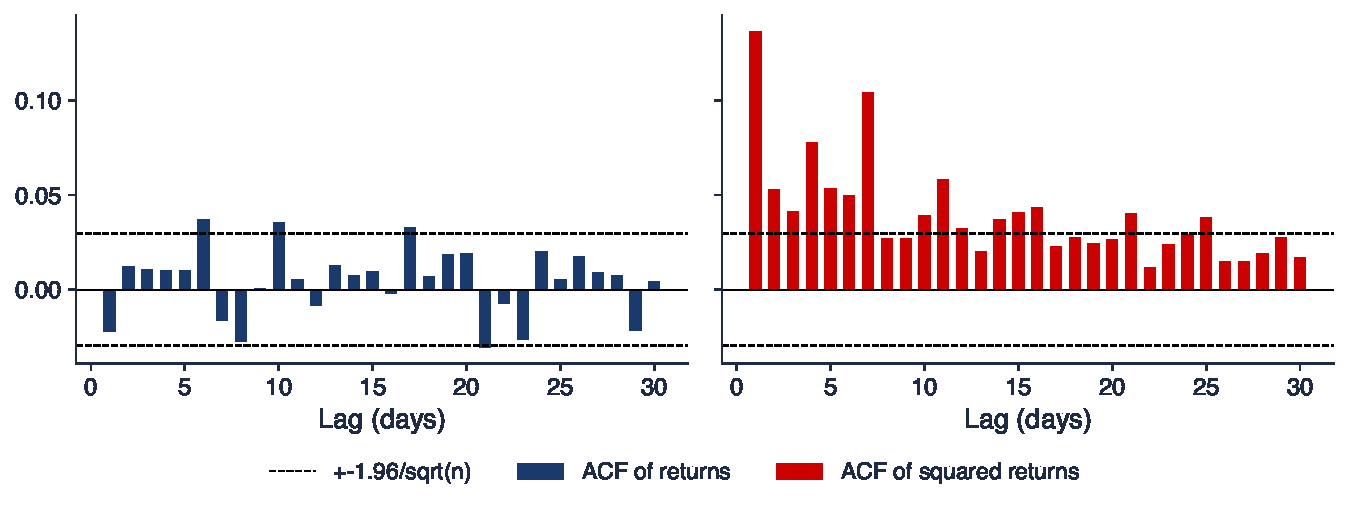
\includegraphics[width=0.97\textwidth,height=0.46\textheight,keepaspectratio]{sfm_ch14_acf.pdf}
\end{center}
\vspace{-0.25cm}
\begin{itemize}
    \item ACF (funcția de autocorelație) a lui $r_t$ și a lui $r_t^2$, decalajele 1--30; linii întrerupte: $\pm 1{,}96/\sqrt{n} = \pm 0{,}030$
    \item Randamentele: $\hat\rho(1) = -0{,}022$, 4 din 30 de decalaje în afara benzii; pătratele: $\hat\rho(1) = 0{,}137$, 15 din 30 în afara benzii
    \item Interpretare: statistica Ljung--Box $Q(10)$ este 20{,}2 pentru $r_t$ și 212{,}7 pentru $r_t^2$ (p $<$\,0{,}001): direcția este greu de prognozat, mărimea mișcării nu
\end{itemize}
\sfmquantlet{Ch_14}{SFM_ch14_garch_efficiency}
\end{frame}

\begin{frame}{GARCH(1,1)-t pentru active cripto și tradiționale}
\itemsize{\footnotesize}
\begin{center}
\scriptsize
\begin{tabular}{lrrrrrrr}
\toprule
& $\hat\omega$ & $\hat\alpha$ & $\hat\beta$ & $\hat\alpha + \hat\beta$ & timp de înjumătățire (zile) & $\hat\nu$ & GJR $\hat\gamma$ ($t$) \\
\midrule
Bitcoin & $0{,}194$ & $0{,}109$ & $0{,}891$ & $1{,}000$ & -- & $3{,}18$ & $-0{,}013$ ($-0{,}72$) \\
Ethereum & $1{,}067$ & $0{,}175$ & $0{,}825$ & $1{,}000$ & -- & $3{,}14$ & $0{,}032$ ($0{,}91$) \\
S\&P 500 & $0{,}024$ & $0{,}173$ & $0{,}820$ & $0{,}993$ & 100 & $5{,}50$ & $0{,}280$ ($7{,}08$) \\
Aur & $0{,}010$ & $0{,}047$ & $0{,}947$ & $0{,}994$ & 113 & $4{,}13$ & $-0{,}051$ ($-3{,}33$) \\
\bottomrule
\end{tabular}
\end{center}
\begin{itemize}
    \item \refBoll{} (\sfmchlink{https://danpele.github.io/SFM/RO/Cursuri/capitol9_modele_arch_garch.pdf}{Capitolul 9}): $\sigma_t^2 = \omega + \alpha\varepsilon_{t-1}^2 + \beta\sigma_{t-1}^2$, inovații Student-t cu $\nu$ grade de libertate; timpul de înjumătățire a unui șoc $\ln 0{,}5/\ln(\alpha + \beta)$
    \begin{itemize}
        \item GJR: un termen suplimentar $\gamma\,\varepsilon_{t-1}^2\mathbb{1}\{\varepsilon_{t-1} < 0\}$; $\gamma > 0$ este efectul de levier al acțiunilor
    \end{itemize}
\end{itemize}
\end{frame}

\begin{frame}{Interpretarea estimărilor GARCH}
\itemsize{\small}
\begin{itemize}
    \item Cripto: $\hat\alpha + \hat\beta = 1$, la limita domeniului: un GARCH integrat (IGARCH; EWMA din \sfmchlink{https://danpele.github.io/SFM/RO/Cursuri/capitol8_estimatori_volatilitate.pdf}{Capitolul 8} este cazul $\omega = 0$)
    \begin{itemize}
        \item un șoc al volatilității nu se stinge în eșantion; nu există o varianță de termen lung finită spre care să revină volatilitatea
        \item S\&P 500 și aurul: timpi de înjumătățire de 100 și 113 zile
    \end{itemize}
    \item $\hat\nu \approx 3{,}18$ pentru Bitcoin: chiar după filtrarea GARCH, cozile sînt foarte groase
    \begin{itemize}
        \item S\&P 500 are $\hat\nu = 5{,}50$
    \end{itemize}
    \item Niciun efect de levier la cripto: $\hat\gamma = -0{,}013$ ($t = -0{,}72$) pentru Bitcoin, față de $0{,}280$ ($t = 7{,}08$) pentru S\&P 500
    \begin{itemize}
        \item aurul are $\hat\gamma < 0$ ($t = -3{,}33$): creșterile prețului cresc volatilitatea mai mult decît scăderile, ca la un activ de refugiu
    \end{itemize}
    \item \refKatsiampa{} compară modele de tip GARCH pentru Bitcoin: cel mai bine se potrivește un model cu o componentă de termen scurt și una de termen lung a volatilității
\end{itemize}
\end{frame}

\begin{frame}{Volatilitatea condiționată: Bitcoin și S\&P 500}
\itemsize{\footnotesize}
\begin{center}
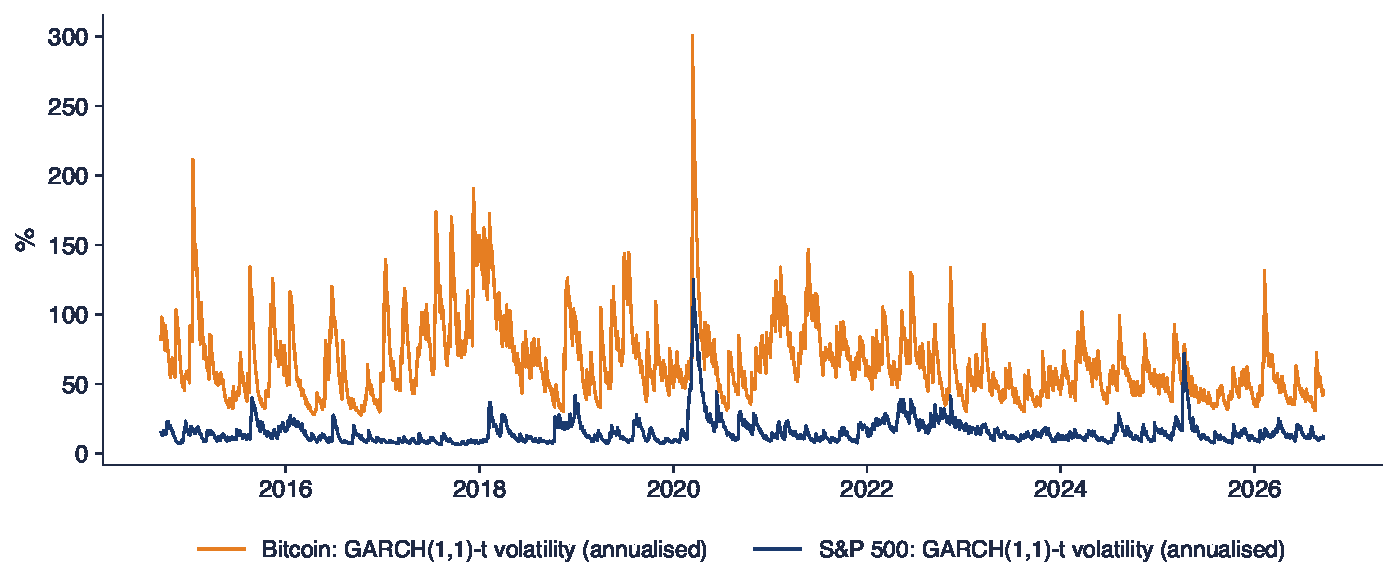
\includegraphics[width=0.97\textwidth,height=0.48\textheight,keepaspectratio]{sfm_ch14_garch_vol.pdf}
\end{center}
\vspace{-0.25cm}
\begin{itemize}
    \item Volatilitatea GARCH(1,1)-t $\hat\sigma_t$, anualizată cu $\sqrt{365}$ (Bitcoin) și $\sqrt{252}$ (S\&P 500)
    \item Interpretare: ambele ating maximul în martie 2020 (301\% și 125\%); pe 18 septembrie 2026, modelul dă 42\% pentru Bitcoin și 12\% pentru S\&P 500
\end{itemize}
\sfmquantlet{Ch_14}{SFM_ch14_garch_efficiency}
\end{frame}

\begin{frame}{Recapitulare: cozi și volatility clustering}
\itemsize{\small}
\begin{itemize}
    \item Cozile cripto sînt groase ($\hat\alpha$ între 2,5 și 3,5), la fel de groase ca formă ca ale S\&P 500; activele cripto diferă prin scală
    \item Volatilitatea se grupează puternic; GARCH-t se estimează cu $\alpha + \beta \approx 1$ (IGARCH)
    \item Niciun efect de levier: veștile bune și cele rele mișcă la fel volatilitatea cripto
\end{itemize}
\end{frame}


%=============================================================================
\section{Este piața cripto eficientă?}
%=============================================================================

\begin{frame}{Eficiența în formă slabă: ce testăm}
\itemsize{\small}
\begin{itemize}
    \item \refFama: pe o piață eficientă în formă slabă, prețurile trecute nu ajută la prognoza randamentelor viitoare (\sfmchlink{https://danpele.github.io/SFM/RO/Cursuri/capitol7_piete_eficiente_mers_aleator_vr.pdf}{Capitolul 7})
    \begin{itemize}
        \item formele eficienței: slabă (prețurile trecute), semi-tare (informația publică), tare (toată informația)
    \end{itemize}
    \item Testele folosite aici
    \begin{itemize}
        \item autocorelația de ordinul întîi $\hat\rho(1)$ și statistica Ljung--Box $Q(10)$
        \item raportul varianțelor \refLM: $\mathrm{VR}(q) = \mathrm{Var}(r_t + \dots + r_{t-q+1})/(q\,\mathrm{Var}(r_t))$, egal cu 1 pentru un mers aleator
        \item $Z^*(q)$: varianta robustă la volatility clustering; respingem la 5\% dacă $|Z^*| > 1{,}96$
    \end{itemize}
    \item VR $> 1$: momentum (tendințe); VR $< 1$: revenire la medie
\end{itemize}
\end{frame}

\begin{frame}{Testele raportului varianțelor pe întregul eșantion}
\itemsize{\scriptsize}
\begin{center}
\scriptsize
\begin{tabular}{lrrrrrr}
\toprule
& $\hat\rho(1)$ & $Q(10)$ (p) & VR(2) & VR(5) & VR(10) & $Z^*(5)$ (p) \\
\midrule
Bitcoin & $-0{,}022$ & $20{,}2$ (0{,}028) & $0{,}977$ & $0{,}991$ & $1{,}027$ & $-0{,}19$ (0{,}853) \\
Ethereum & $-0{,}012$ & $22{,}7$ (0{,}012) & $0{,}988$ & $1{,}067$ & $1{,}137$ & $1{,}17$ (0{,}241) \\
S\&P 500 & $-0{,}126$ & $236{,}1$ ($<$\,0{,}001) & $0{,}875$ & $0{,}849$ & $0{,}813$ & $-1{,}28$ (0{,}201) \\
\bottomrule
\end{tabular}
\end{center}
\begin{center}
\scriptsize
\begin{tabular}{llrrrr}
\toprule
& perioada & $n$ & $\hat\rho(1)$ & VR(5) & $Z^*(5)$ (p) \\
\midrule
Bitcoin & 2014--2017 & 1\,201 & $0{,}028$ & $0{,}975$ & $-0{,}23$ (0{,}815) \\
Bitcoin & 2018--2021 & 1\,460 & $-0{,}057$ & $0{,}981$ & $-0{,}25$ (0{,}801) \\
Bitcoin & 2022--2026 & 1\,721 & $-0{,}026$ & $1{,}013$ & $0{,}18$ (0{,}856) \\
Ethereum & 2016--2017 & 730 & $0{,}034$ & $1{,}127$ & $1{,}03$ (0{,}303) \\
Ethereum & 2018--2021 & 1\,460 & $-0{,}064$ & $0{,}997$ & $-0{,}04$ (0{,}971) \\
Ethereum & 2022--2026 & 1\,721 & $-0{,}015$ & $1{,}014$ & $0{,}20$ (0{,}844) \\
\bottomrule
\end{tabular}
\end{center}
\begin{itemize}
    \item Interpretare: niciun test VR nu respinge mersul aleator, în nicio subperioadă; testul Ljung--Box respinge slab la cripto deoarece ignoră volatility clustering
\end{itemize}
\end{frame}

\begin{frame}{Eficiența în timp}
\itemsize{\footnotesize}
\begin{center}
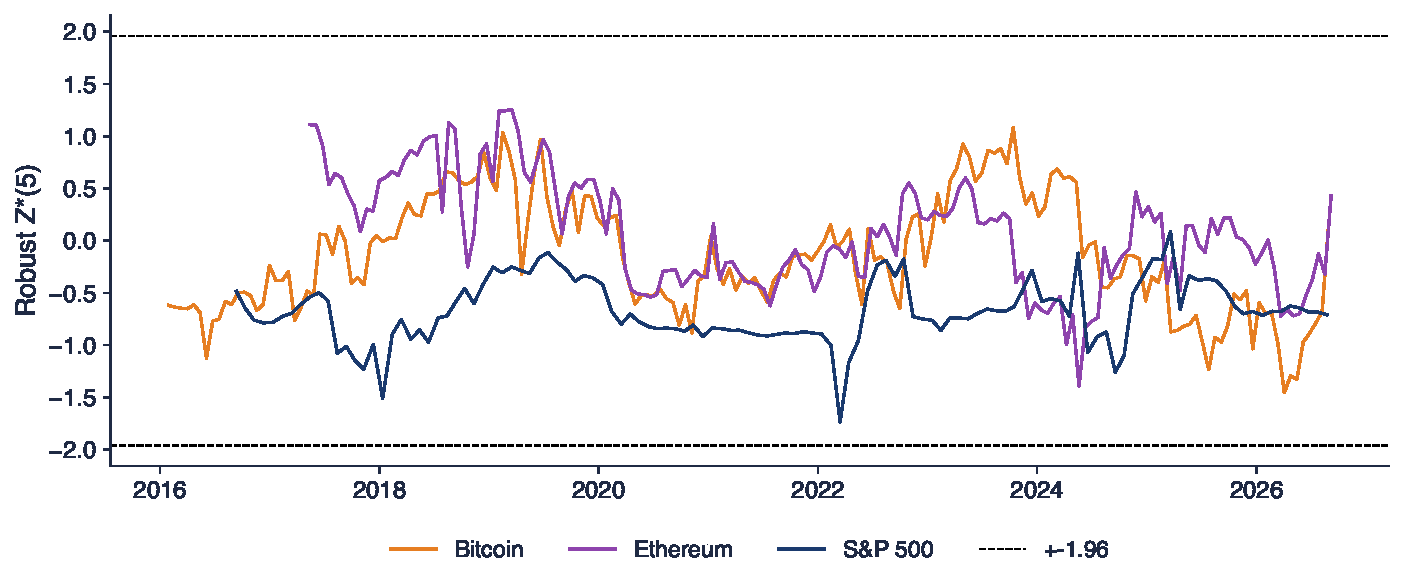
\includegraphics[width=0.97\textwidth,height=0.46\textheight,keepaspectratio]{sfm_ch14_rolling_vr.pdf}
\end{center}
\vspace{-0.25cm}
\begin{itemize}
    \item Statistica robustă $Z^*(5)$ pe ferestre de 500 de observații, o fereastră la fiecare 21 de observații (ca în \sfmchlink{https://danpele.github.io/SFM/RO/Cursuri/capitol7_piete_eficiente_mers_aleator_vr.pdf}{Capitolul 7})
    \item Interpretare: la Bitcoin, 0{,}0\% din 185 de ferestre resping; cu statistica i.i.d.\ $Z(5)$, proporția ar fi 1{,}6\% pentru Bitcoin și 21{,}7\% pentru S\&P 500: ignorarea volatility clustering produce respingeri false
\end{itemize}
\sfmquantlet{Ch_14}{SFM_ch14_garch_efficiency}
\end{frame}

\begin{frame}{Evoluția eficienței}
\itemsize{\small}
\begin{itemize}
    \item \refUrquhart: Bitcoin a fost ineficient în 2010--2016 ca întreg, dar s-a apropiat de eficiență după 2013
    \begin{itemize}
        \item \refNC: o transformare de tip putere a acelorași randamente trece testele: verdictul inițial era fragil
        \item \refTL: o măsură ajustată a ineficienței; piețele cripto au devenit mai eficiente după 2017
    \end{itemize}
    \item Datele noastre (din 2014): VR(5) între 0{,}78 și 1{,}17 pe ferestre mobile; nicio respingere robustă
    \begin{itemize}
        \item piața a crescut, au venit arbitrajorii, au apărut derivatele și ETF-urile: perspectiva piețelor adaptive din \sfmchlink{https://danpele.github.io/SFM/RO/Cursuri/capitol11_piete_fractale_memorie_lunga.pdf}{Capitolul 11}
    \end{itemize}
    \item Eficiența în formă slabă nu este eficiență în general: prețurile pot fi imprevizibile și totuși departe de orice valoare fundamentală
\end{itemize}
\end{frame}

\begin{frame}{Studiu de caz: tranzacționare și arbitraj între exchange-uri}
\itemsize{\small}
\begin{itemize}
    \item \refMS: date tick-by-tick de pe 34 de exchange-uri din 19 țări, 2017--2018
    \begin{itemize}
        \item \textbf{arbitraj}: cumpărăm unde prețul este mic, vindem unde este mare; pe o piață eficientă diferența se închide repede
    \end{itemize}
    \item Rezultatele
    \begin{itemize}
        \item diferențe mari și persistente de preț între țări (Coreea, Japonia și SUA), mult mai mici în interiorul unei țări
        \item diferențele se deschid cînd Bitcoin crește, iar controlul capitalurilor face arbitrajul dificil
        \item o componentă comună explică cea mai mare parte a fluxului de ordine: prețurile sînt determinate de o piață globală
    \end{itemize}
    \item Lecția: „legea prețului unic” nu funcționează acolo unde banii nu circulă liber; un test statistic pe o singură serie nu poate vedea asta
\end{itemize}
\end{frame}

\begin{frame}{Studiu de caz: este Bitcoin cu adevărat independent de Tether?}
\itemsize{\small}
\begin{itemize}
    \item \refGS: înregistrările din blockchain ale Bitcoin și ale stablecoin-ului Tether (USDT), 2017--2018
    \begin{itemize}
        \item întrebarea: a fost folosit USDT nou emis pentru a cumpăra Bitcoin după scăderi de preț?
    \end{itemize}
    \item Rezultatele
    \begin{itemize}
        \item cumpărările cu Tether au venit după scăderi ale pieței și au fost urmate de creșteri ale prețului
        \item fluxurile proveneau în principal de la un singur cont mare de pe un singur exchange (Bitfinex)
        \item orele cu astfel de fluxuri explică o parte mare a creșterii din 2017
    \end{itemize}
    \item Similar: manipularea exchange-ului Mt.~Gox în 2013 \refGHMO. Lecția: datele din blockchain permit teste imposibile pe piețele de acțiuni
\end{itemize}
\end{frame}

\begin{frame}{Recapitulare: este piața cripto eficientă?}
\itemsize{\small}
\begin{itemize}
    \item Testele VR robuste nu resping mersul aleator pentru Bitcoin și Ethereum din 2014
    \item Studiile timpurii au găsit ineficiență; piața a devenit mai eficientă pe măsură ce a crescut
    \item Diferențele de arbitraj între țări și manipularea arată limitele testelor de formă slabă
\end{itemize}
\end{frame}


%=============================================================================
\section{Corelația cu acțiunile și aurul}
%=============================================================================

\begin{frame}{Măsurarea corelației între calendare diferite}
\itemsize{\small}
\begin{itemize}
    \item Bitcoin se tranzacționează 7 zile pe săptămînă, S\&P 500 și aurul 5: întîi unim \textbf{prețurile} în zilele comune, apoi calculăm randamentele
    \begin{itemize}
        \item randamentul Bitcoin de luni acoperă atunci perioada vineri--luni, ca și randamentul S\&P 500
        \item unirea randamentelor, în schimb, ar elimina mișcările Bitcoin din weekend
    \end{itemize}
    \item Închideri \textbf{asincrone}: Bitcoin la miezul nopții UTC, S\&P 500 la ora 16:00 la New York
    \begin{itemize}
        \item randamentele săptămînale (vineri--vineri) reduc această problemă; le raportăm pe ambele
    \end{itemize}
    \item \textbf{Corelația mobilă}: corelația de selecție pe ultimele 250 de zile comune, recalculată în fiecare zi
    \begin{itemize}
        \item eroarea standard este circa $(1 - \rho^2)/\sqrt{250} \approx 0{,}06$: mișcările sub 0,1 sînt zgomot
    \end{itemize}
\end{itemize}
\end{frame}

\begin{frame}{Corelația mobilă cu acțiunile și aurul}
\itemsize{\footnotesize}
\begin{center}
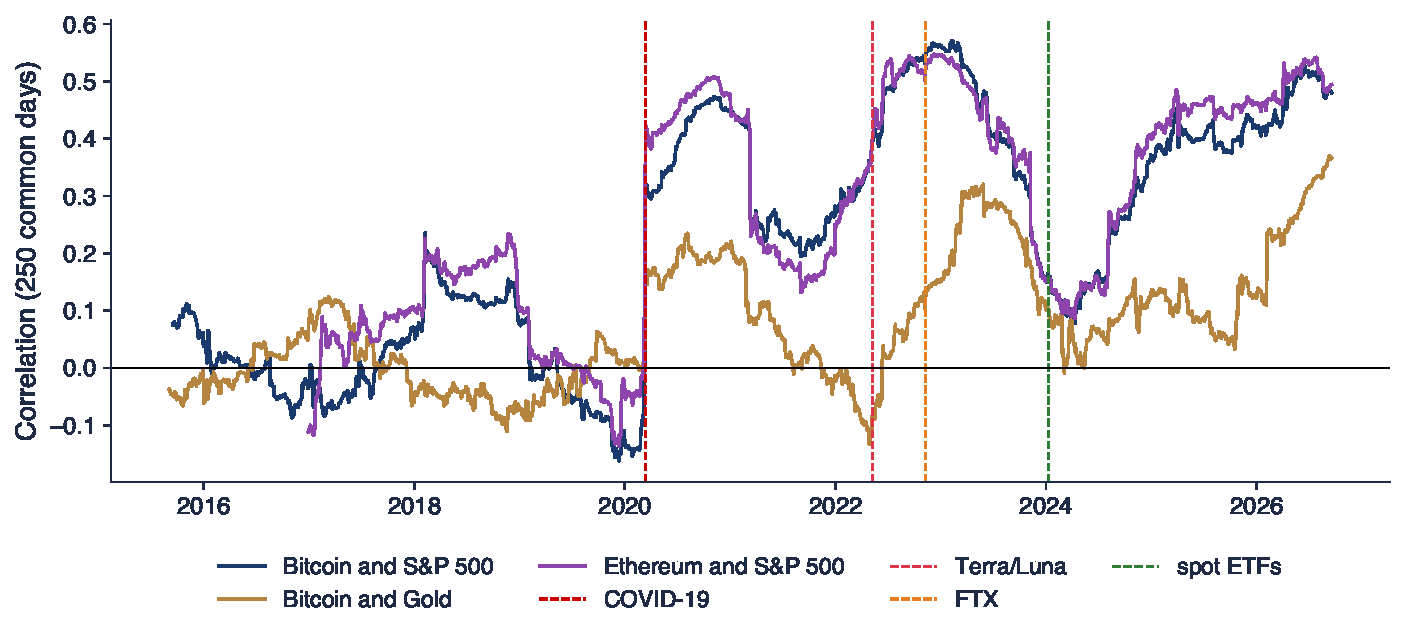
\includegraphics[width=0.97\textwidth,height=0.48\textheight,keepaspectratio]{sfm_ch14_rolling_corr.pdf}
\end{center}
\vspace{-0.25cm}
\begin{itemize}
    \item Randamente logaritmice zilnice în zilele comune; ferestre de 250 de zile; linii întrerupte: COVID-19, Terra/Luna, FTX și ETF-urile spot
    \item Interpretare: Bitcoin și S\&P 500 erau necorelate înainte de 2020 (0{,}02) și corelate pozitiv după (0{,}39); maximul, 0{,}57, a apărut pe 9 februarie 2023; legătura cu aurul rămîne slabă
\end{itemize}
\sfmquantlet{Ch_14}{SFM_ch14_correlation}
\end{frame}

\begin{frame}{Corelația an cu an}
\itemsize{\footnotesize}
\begin{center}
\scriptsize
\begin{tabular}{lrrrrrrr}
\toprule
Bitcoin cu & 2019 & 2020 & 2021 & 2022 & 2023 & 2024 & 2025 \\
\midrule
S\&P 500 & $-0{,}11$ & $0{,}45$ & $0{,}26$ & $0{,}56$ & $0{,}16$ & $0{,}36$ & $0{,}42$ \\
aurul & $0{,}01$ & $0{,}21$ & $-0{,}02$ & $0{,}15$ & $0{,}12$ & $0{,}12$ & $0{,}12$ \\
Ethereum cu S\&P 500 & $-0{,}02$ & $0{,}47$ & $0{,}20$ & $0{,}55$ & $0{,}15$ & $0{,}40$ & $0{,}46$ \\
\bottomrule
\end{tabular}
\end{center}
\begin{itemize}
    \item Întreaga perioadă: zilnic 0{,}24, săptămînal 0{,}19 pentru Bitcoin și S\&P 500
    \begin{itemize}
        \item închiderile asincrone nu explică corelația: randamentele săptămînale dau o valoare apropiată
    \end{itemize}
    \item Interpretare
    \begin{itemize}
        \item din 2020, activele cripto se comportă ca active riscante: scad odată cu acțiunile cînd dobînzile cresc (2022)
        \item schimbarea coincide cu intrarea investitorilor instituționali; beneficiul diversificării măsurat înainte de 2020 nu se mai păstrează
    \end{itemize}
\end{itemize}
\end{frame}

\begin{frame}{Trei episoade de criză}
\itemsize{\footnotesize}
\begin{center}
\scriptsize
\begin{tabular}{llrrrrr}
\toprule
Episodul & perioada & Bitcoin & Ethereum & S\&P 500 & aur & cea mai proastă zi Bitcoin \\
\midrule
COVID-19 & 19 februarie 2020 -- 23 martie 2020 & $-40{,}6$ & $-65{,}5$ & $-41{,}4$ & $0{,}3$ & $-46{,}5$ \\
Terra/Luna & 5 mai 2022 -- 12 mai 2022 & $-23{,}0$ & $-33{,}8$ & $-5{,}4$ & $-3{,}0$ & $-11{,}7$ \\
FTX & 5 noiembrie 2022 -- 21 noiembrie 2022 & $-29{,}9$ & $-38{,}4$ & $4{,}6$ & $3{,}4$ & $-15{,}5$ \\
\bottomrule
\end{tabular}
\end{center}
\begin{itemize}
    \item Randamente logaritmice cumulate în \% de la prima la ultima închidere; cea mai proastă zi: cel mai mic randament logaritmic zilnic al Bitcoin
    \item Interpretare
    \begin{itemize}
        \item COVID-19 (un șoc global): activele cripto au scăzut cît acțiunile, aurul nu s-a mișcat
        \item Terra/Luna (mai 2022) și FTX (un exchange care a dat faliment în noiembrie 2022): șocuri specifice cripto; activele cripto au scăzut cu un sfert sau mai mult, S\&P 500 mult mai puțin sau deloc
        \item dependența este asimetrică: crahurile acțiunilor ajung la cripto, crahurile cripto rareori ajung la acțiuni
    \end{itemize}
\end{itemize}
\end{frame}

\begin{frame}{Acoperire sau refugiu?}
\itemsize{\small}
\begin{itemize}
    \item \refBL: o \textbf{acoperire} (hedge) este necorelată sau corelată negativ cu acțiunile în medie; un \textbf{refugiu} (safe haven) este astfel în timpul crahurilor
    \begin{itemize}
        \item testul: randamentul mediu în cele mai proaste 5\% dintre zilele S\&P 500 (151 de zile comune, S\&P 500 sub $-1{,}65\%$, în medie $-2{,}70\%$)
    \end{itemize}
    \item Bitcoin: $-2{,}77\%$ în acele zile ($t = -4{,}89$, p $<$\,0{,}001); negativ în 70\% dintre ele
    \begin{itemize}
        \item aurul: 0{,}10\% ($t = 0{,}86$, p 0{,}394)
    \end{itemize}
    \item Interpretare: Bitcoin nu este un activ de refugiu; în cele mai proaste zile ale acțiunilor scade cît S\&P 500; aurul își păstrează valoarea
    \item Narațiunea „aurului digital” nu este susținută de datele acestui eșantion
\end{itemize}
\end{frame}

\begin{frame}{Recapitulare: corelația cu acțiunile și aurul}
\itemsize{\small}
\begin{itemize}
    \item Unim prețurile în zilele comune, apoi calculăm randamentele; verificăm și randamentele săptămînale
    \item Corelația cu acțiunile: circa 0 înainte de 2020, circa 0{,}39 după
    \item Bitcoin nu este nici acoperire, nici refugiu pentru acțiuni în acest eșantion
\end{itemize}
\end{frame}


%=============================================================================
\section{Bule și crahuri}
%=============================================================================

\begin{frame}{Drawdown-ul}
\itemsize{\small}
\begin{itemize}
    \item \textbf{Drawdown}: $D_t = P_t/\max_{s \le t} P_s - 1$, pierderea față de ultimul maxim istoric (\sfmchlink{https://danpele.github.io/SFM/RO/Cursuri/capitol1_date_randamente_indicatori.pdf}{Capitolul 1})
    \begin{itemize}
        \item \textbf{drawdown maxim}: $\min_t D_t$; \textbf{timpul sub apă} (time under water): zilele pînă la un nou maxim istoric
    \end{itemize}
    \item O pierdere $d$ cere un cîștig $d/(1 - d)$ pentru recuperare
    \begin{itemize}
        \item $d = 75\%$: $0{,}75/0{,}25 = 300\%$; $d = 80\%$: 400\%
        \item cel mai adînc drawdown al Bitcoin în datele noastre: $-83{,}4\%$ (15 decembrie 2018); recuperarea a cerut un cîștig de 502\%
    \end{itemize}
    \item Drawdown-urile depind de traiectorie, nu doar de distribuția randamentelor: volatilitatea mare și gruparea ei produc drawdown-uri adînci
\end{itemize}
\end{frame}

\begin{frame}{Drawdown-urile Bitcoin, Ethereum și S\&P 500}
\itemsize{\footnotesize}
\begin{center}
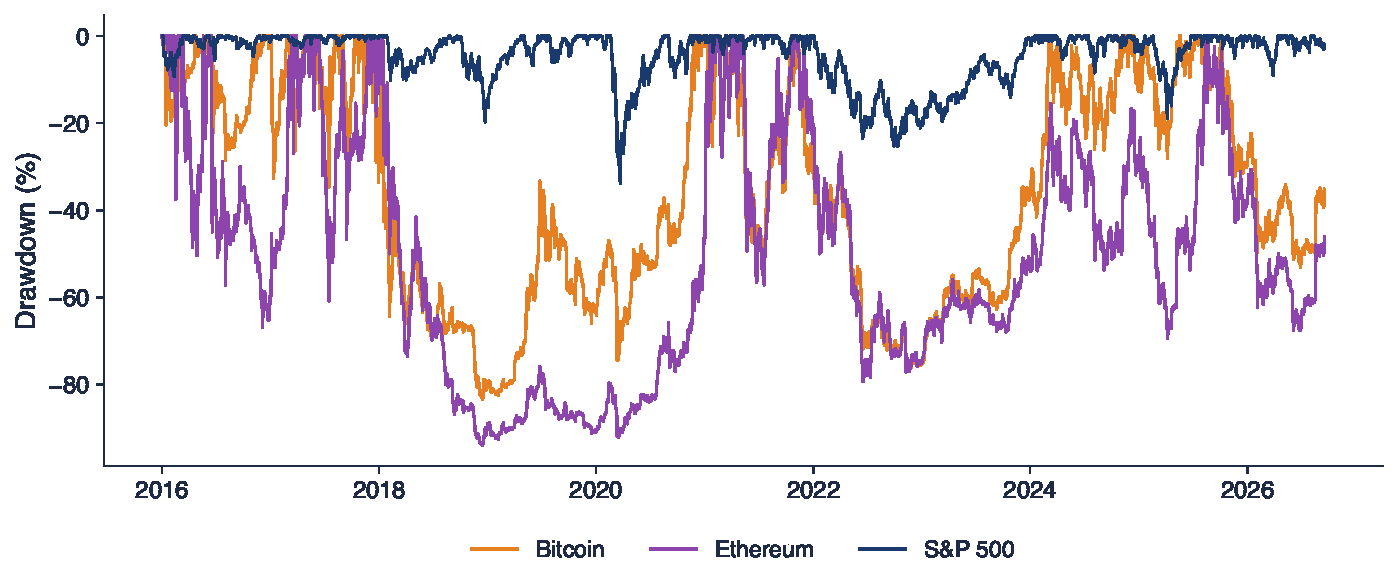
\includegraphics[width=0.97\textwidth,height=0.46\textheight,keepaspectratio]{sfm_ch14_drawdowns.pdf}
\end{center}
\vspace{-0.25cm}
\begin{itemize}
    \item Închideri zilnice din 2016; drawdown-uri maxime: Bitcoin $-83{,}4\%$, Ethereum $-94{,}0\%$, S\&P 500 $-33{,}9\%$
    \item Interpretare: Bitcoin a petrecut 76\% din zile la peste 10\% sub maximul istoric, Ethereum 90\%, S\&P 500 16\%; pe 18 septembrie 2026, Bitcoin era cu 35{,}2\% sub maximul istoric
\end{itemize}
\sfmquantlet{Ch_14}{SFM_ch14_bubbles_etf}
\end{frame}

\begin{frame}{Marile drawdown-uri ale Bitcoin}
\itemsize{\footnotesize}
\begin{center}
\scriptsize
\begin{tabular}{lrlrrlr}
\toprule
Maxim & USD & minim & USD & adîncime (\%) & nou maxim & zile sub apă \\
\midrule
2014-09-17 & 457 & 2015-01-14 & 178 & $-61{,}1$ & 2015-12-15 & 454 \\
2017-12-16 & 19\,497 & 2018-12-15 & 3\,237 & $-83{,}4$ & 2020-11-30 & 1080 \\
2021-04-13 & 63\,503 & 2021-07-20 & 29\,807 & $-53{,}1$ & 2021-10-19 & 189 \\
2021-11-08 & 67\,567 & 2022-11-21 & 15\,787 & $-76{,}6$ & 2024-03-04 & 847 \\
2025-10-06 & 124\,753 & 2026-06-30 & 58\,559 & $-53{,}1$ & încă nu & -- \\
\bottomrule
\end{tabular}
\end{center}
\begin{itemize}
    \item Episoadele din septembrie 2014 cu drawdown de peste 50\%; datele în formatul an-lună-zi
    \item Interpretare
    \begin{itemize}
        \item 5 scăderi de peste jumătate în doisprezece ani: un crah de această mărime este un eveniment obișnuit, nu unul rar
        \item maximele din 2017 și 2021 au fost recuperate după 1080 și, respectiv, 847 de zile
    \end{itemize}
\end{itemize}
\end{frame}

\begin{frame}{Bulele și ideea log-periodică}
\itemsize{\footnotesize}
\begin{columns}[T]
\begin{column}{0.66\textwidth}
\begin{itemize}
    \item \textbf{Bulă}: un preț mult peste valoarea fundamentală, susținut de așteptarea unei revînzări la un preț mai mare
    \begin{itemize}
        \item \refCF: valoarea fundamentală a Bitcoin este zero; prețul său arată bule speculative
    \end{itemize}
    \item Legea de putere log-periodică (LPPL) \refJLS: înaintea unui crah, $\ln P_t \approx A + B(t_c - t)^m + C(t_c - t)^m\cos(\omega\ln(t_c - t) - \phi)$
    \begin{itemize}
        \item o creștere mai rapidă decît cea exponențială, cu oscilații tot mai dese; $t_c$: momentul critic
    \end{itemize}
    \item Atenție: șapte parametri, multe optime locale, iar $t_c$ este cel mai incert dintre ei; ajustările par convingătoare abia după crah
\end{itemize}
\end{column}
\begin{column}{0.31\textwidth}
\centering
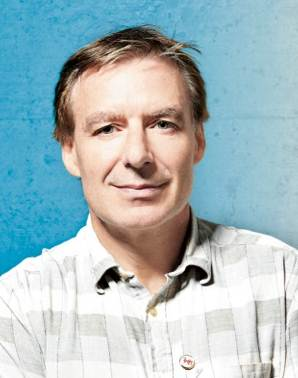
\includegraphics[height=0.36\textheight]{ch14_sornette_2012.jpg}\\[1mm]
\imgcap{Didier Sornette}
\imgcredit{https://commons.wikimedia.org/wiki/File:Didier_Sornette.jpg}{Foto: Didier Sornette (2012); CC BY-SA 3.0 DE; Wikimedia Commons}
\end{column}
\end{columns}
\end{frame}

\begin{frame}{Recapitulare: bule și crahuri}
\itemsize{\small}
\begin{itemize}
    \item Drawdown $= P_t/\max P - 1$; o scădere $d$ cere un cîștig $d/(1 - d)$
    \item Bitcoin a pierdut mai mult de jumătate din valoare de 5 ori din 2014
    \item Modelele de bule sînt descrieri utile, dar nesigure pentru datarea unui crah
\end{itemize}
\end{frame}


%=============================================================================
\section{ETF-urile spot pe Bitcoin}
%=============================================================================

\begin{frame}{Ianuarie 2024: Bitcoin intră la bursă}
\itemsize{\footnotesize}
\begin{columns}[T]
\begin{column}{0.62\textwidth}
\begin{itemize}
    \item \textbf{ETF} (exchange-traded fund): un fond ale cărui unități se tranzacționează la bursă; \textbf{spot}: deține activul însuși, nu contracte futures
    \begin{itemize}
        \item 10 ianuarie 2024: SEC (Securities and Exchange Commission) aprobă 11 ETF-uri spot pe Bitcoin \refSEC; tranzacționarea începe pe 11 ianuarie
    \end{itemize}
    \item De ce contează
    \begin{itemize}
        \item fondurile de pensii și consultanții pot deține Bitcoin printr-un instrument financiar reglementat
        \item unitățile ETF se tranzacționează doar în zilele lucrătoare: o parte a tranzacționării se mută în orele bursei
    \end{itemize}
    \item Întrebarea statistică: s-au schimbat volatilitatea Bitcoin, tiparul ei de weekend sau legătura cu acțiunile?
\end{itemize}
\end{column}
\begin{column}{0.35\textwidth}
\centering
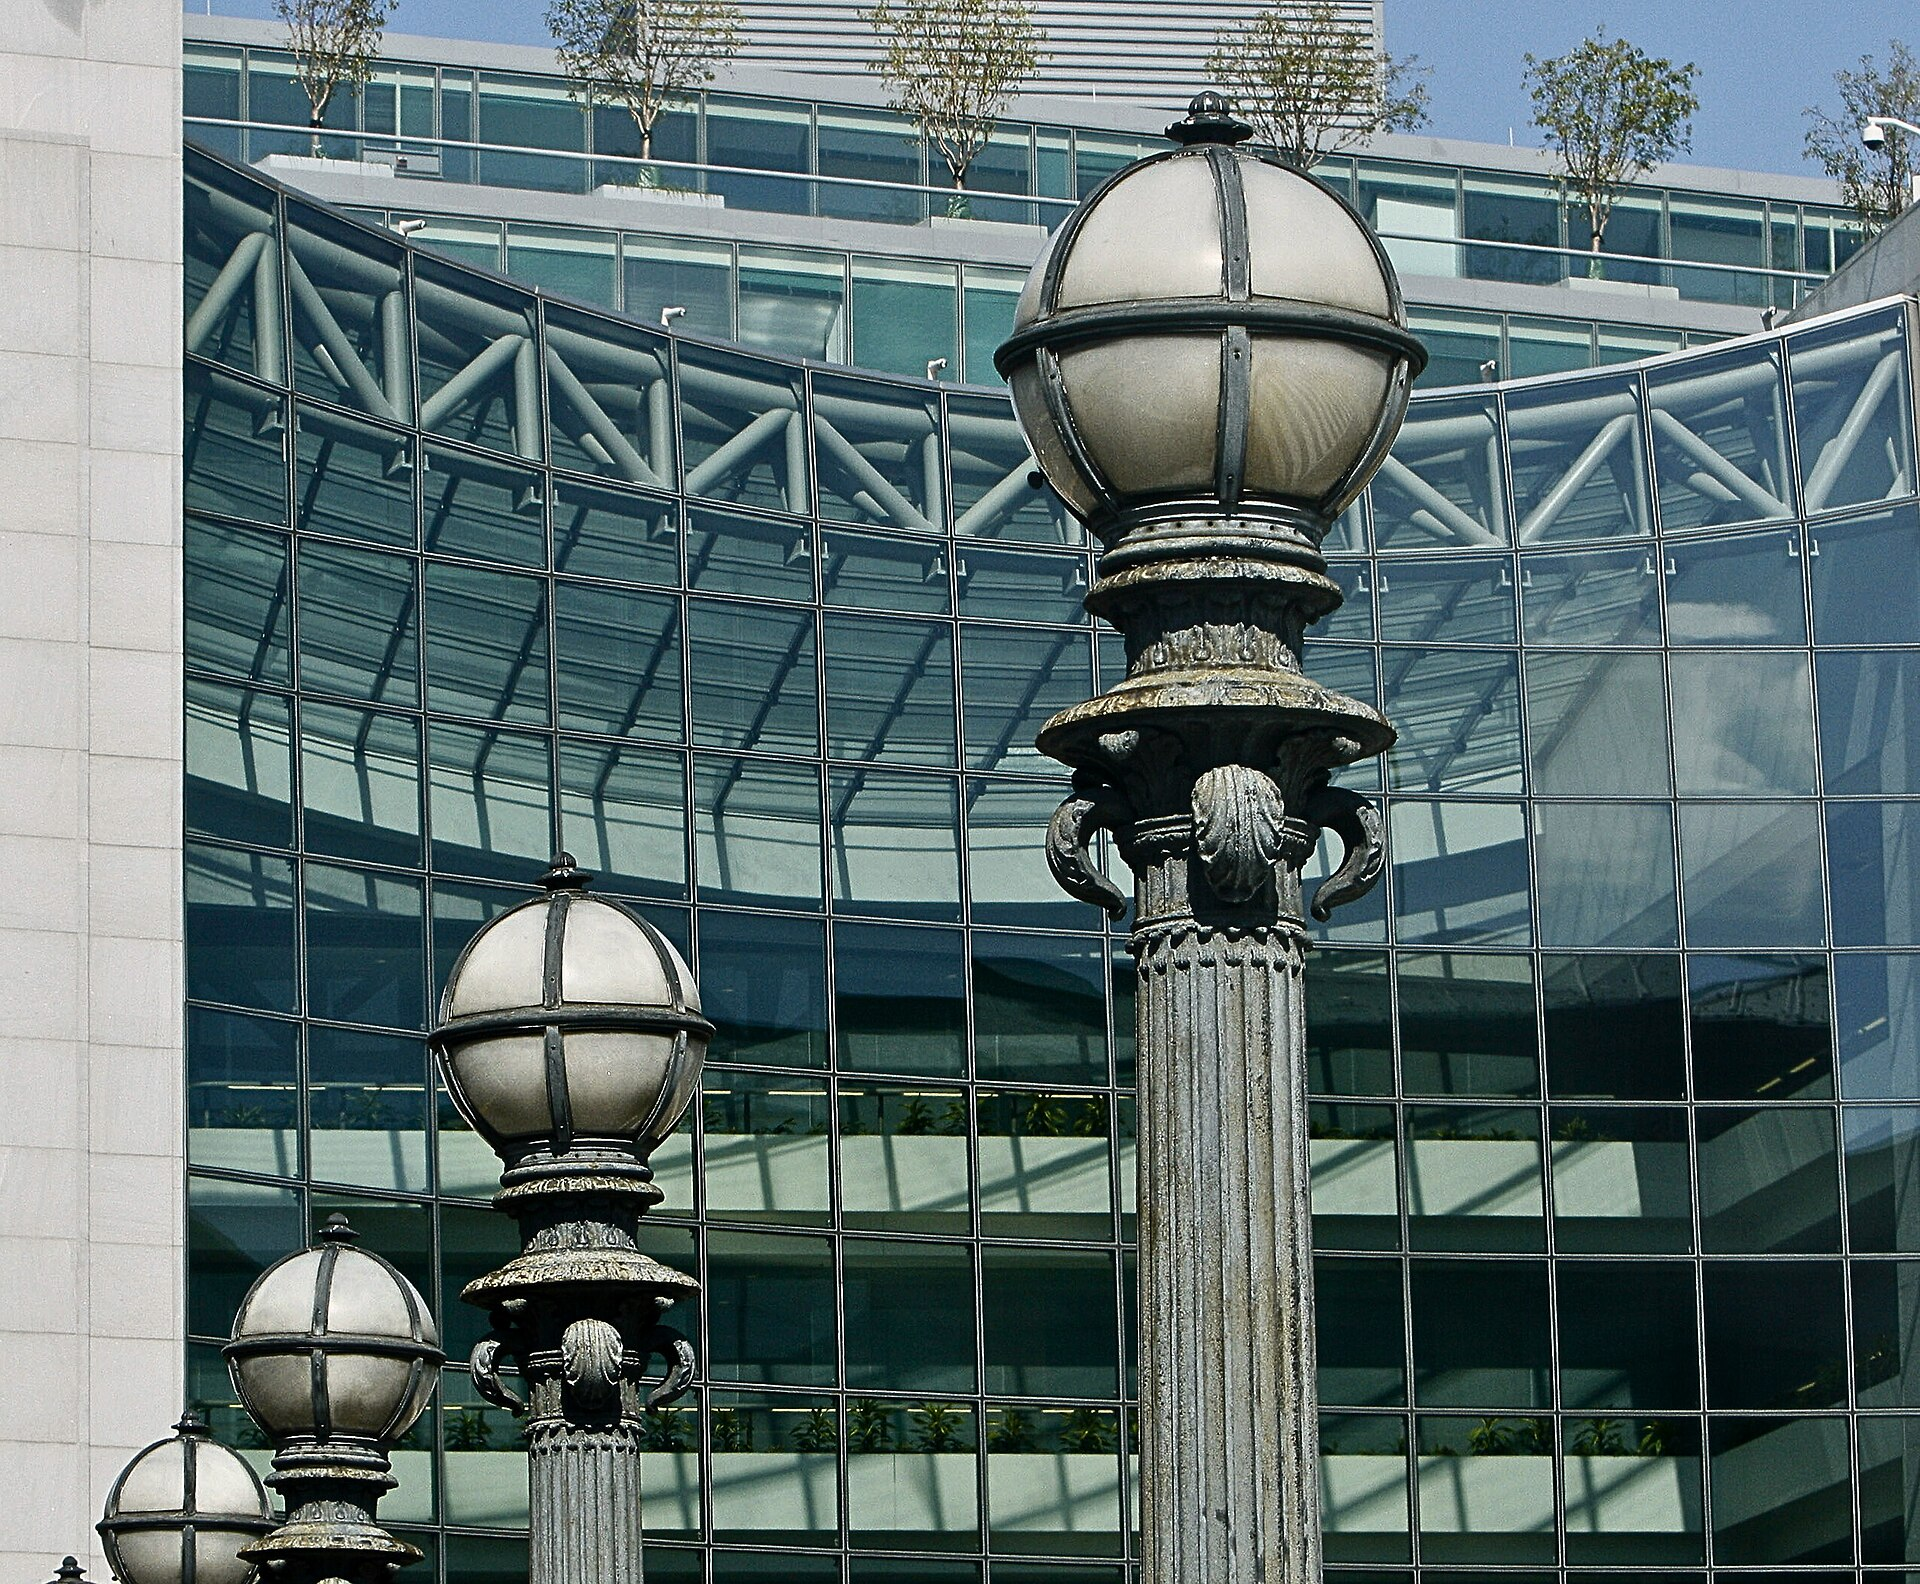
\includegraphics[height=0.34\textheight]{ch14_sec_hq_2008.jpg}\\[1mm]
\imgcap{Sediul SEC, Washington, D.C.}
\imgcredit{https://commons.wikimedia.org/wiki/File:Facade_of_the_U.S._Securities_and_Exchange_Commission_headquarters,_Washington,_D.C.jpg}{Foto: David (dbking) (2008); CC BY 2.0; Wikimedia Commons}
\end{column}
\end{columns}
\end{frame}

\begin{frame}{Volatilitatea și ponderea weekendului în jurul ETF-urilor}
\itemsize{\footnotesize}
\begin{center}
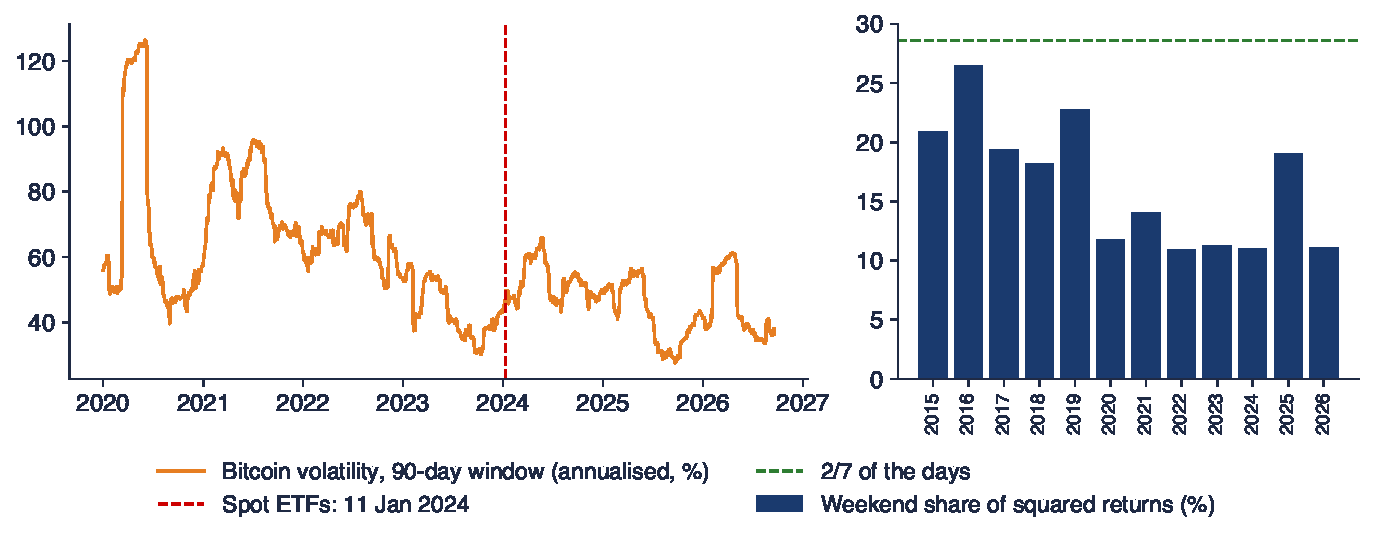
\includegraphics[width=0.97\textwidth,height=0.46\textheight,keepaspectratio]{sfm_ch14_etf.pdf}
\end{center}
\vspace{-0.25cm}
\begin{itemize}
    \item Stînga: volatilitatea Bitcoin pe ferestre de 90 de zile, anualizată cu $\sqrt{365}$. Dreapta: ponderea weekendului în suma pătratelor randamentelor, pe ani (2/7 dacă fiecare zi ar avea aceeași varianță)
    \item Interpretare: volatilitatea a continuat să scadă după ianuarie 2024, dar scădea deja de dinainte; ponderea weekendului este mult sub 2/7 din 2020
\end{itemize}
\sfmquantlet{Ch_14}{SFM_ch14_bubbles_etf}
\end{frame}

\begin{frame}{Înainte și după: o comparație simplă}
\itemsize{\footnotesize}
\begin{center}
\footnotesize
\begin{tabular}{lrr}
\toprule
Bitcoin & doi ani înainte & doi ani după \\
\midrule
volatilitatea anuală (\%) & $55{,}2$ & $47{,}5$ \\
varianța weekend/zile lucrătoare & $0{,}30$ & $0{,}42$ \\
corelația cu S\&P 500 & $0{,}45$ & $0{,}37$ \\
GARCH(1,1)-t $\hat\alpha + \hat\beta$ & $1{,}000$ & $0{,}97$ \\
\bottomrule
\end{tabular}
\end{center}
\begin{itemize}
    \item Ferestrele: 11 ianuarie 2022 -- 10 ianuarie 2024 (729 de zile) și 11 ianuarie 2024 -- 10 ianuarie 2026 (730 de zile)
    \item Testul Brown--Forsythe al egalității varianțelor: statistica 1{,}22, p $= 0{,}27$: scăderea volatilității nu este semnificativă
    \item Interpretare
    \begin{itemize}
        \item o comparație înainte--după nu este un efect cauzal: dobînzile, halving-ul din aprilie 2024 și alegerile din SUA s-au schimbat în același timp
        \item un studiu credibil are nevoie de un grup de control (de exemplu monede fără ETF) sau de date intrazilnice în jurul deschiderii bursei
    \end{itemize}
\end{itemize}
\end{frame}

\begin{frame}{Cît de bine urmărește un ETF prețul Bitcoin?}
\itemsize{\small}
\begin{itemize}
    \item IBIT (iShares Bitcoin Trust), închiderea ajustată, și Bitcoin, prețuri unite în cele 671 de zile de tranzacționare ale ETF-ului
    \begin{itemize}
        \item corelația randamentelor zilnice 0{,}91; panta IBIT în funcție de Bitcoin 0{,}94
        \item \textbf{tracking error}: abaterea standard anualizată a diferenței de randament, 20{,}8\%
    \end{itemize}
    \item De ce nu 1: cele două închideri sînt la patru ore distanță (ora 16:00 la New York față de miezul nopții UTC)
    \begin{itemize}
        \item pe o săptămînă diferența se compensează; fondul deține Bitcoin unu la unu, minus un comision mic
    \end{itemize}
    \item Lecția: un tracking error mare poate fi un artefact de măsurare; aliniem orele înainte de a judeca un fond
\end{itemize}
\end{frame}

\begin{frame}{Recapitulare: ETF-urile spot pe Bitcoin}
\itemsize{\small}
\begin{itemize}
    \item Ianuarie 2024: Bitcoin devine accesibil prin ETF-uri reglementate
    \item Volatilitatea a scăzut (de la 55{,}2\% la 47{,}5\%), nesemnificativ; cauzalitatea nu este identificată
    \item Orele de închidere asincrone măresc tracking error-ul randamentelor zilnice
\end{itemize}
\end{frame}


%=============================================================================
\section{Stablecoins}
%=============================================================================

\begin{frame}{Ce este un stablecoin?}
\itemsize{\footnotesize}
\begin{center}
\scriptsize
\begin{tabular}{>{\raggedright\arraybackslash}p{2.2cm}>{\raggedright\arraybackslash}p{4.4cm}>{\raggedright\arraybackslash}p{2.0cm}>{\raggedright\arraybackslash}p{2.4cm}}
\toprule
Tipul & cum se menține paritatea & exemple & riscul \\
\midrule
garantat cu monedă fiduciară (fiat-backed) & rezerve în dolari, depozite și titluri de stat; deținătorii răscumpără 1 monedă pentru 1 USD la emitent & USDT, USDC & rezervele și banca la care sînt păstrate \\
garantat cu active cripto (crypto-backed) & credite supra-garantate cu active cripto, lichidate automat de contracte inteligente & DAI & o prăbușire a garanției \\
algoritmic & fără rezerve: un algoritm emite și arde o a doua monedă pentru a ține prețul la 1 USD & UST (Terra) & o retragere masivă (run) care distruge ambele monede \\
\bottomrule
\end{tabular}
\end{center}
\begin{itemize}
    \item \textbf{Stablecoin}: un activ cripto conceput să păstreze un preț fix, de obicei 1 USD (\textbf{paritatea}, peg)
    \begin{itemize}
        \item folosit ca numerar pe exchange-uri și pentru plăți transfrontaliere; DefiLlama clasifică azi 91{,}3\% din ofertă ca garantată fiat și 8{,}7\% ca garantată cripto
    \end{itemize}
\end{itemize}
\end{frame}

\begin{frame}{Menținerea parității: arbitrajul}
\itemsize{\small}
\begin{itemize}
    \item Piața primară: tranzacționari autorizați creează o monedă pentru 1 USD la emitent sau o răscumpără pentru 1 USD
    \begin{itemize}
        \item prețul 0,99 pe exchange-uri: cumpărăm la 0,99, răscumpărăm la 1,00, profit 1 cent: cererea împinge prețul înapoi în sus
        \item prețul 1,01: creăm la 1,00, vindem la 1,01: oferta împinge prețul în jos
    \end{itemize}
    \item \refLVN: paritatea Tether se menține prin acest arbitraj; prime apar cînd investitorii se refugiază în stablecoins în perioadele de scădere cripto
    \begin{itemize}
        \item \refMZZ: cu puțini arbitrajori autorizați, retragerile masive sînt mai puțin probabile, dar abaterile durează mai mult
    \end{itemize}
    \item Arbitrajul funcționează doar cîtă vreme investitorii cred că răscumpărarea la 1 USD va fi onorată: o paritate este o promisiune
\end{itemize}
\end{frame}

\begin{frame}{Oferta de stablecoins}
\itemsize{\footnotesize}
\begin{center}
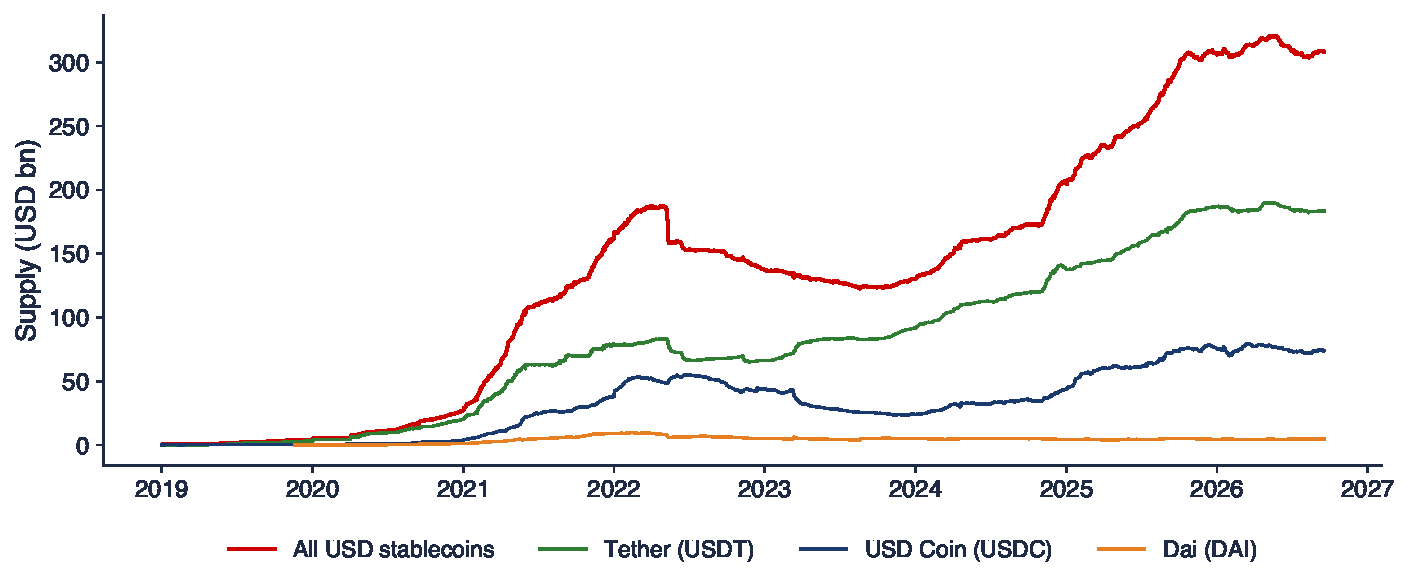
\includegraphics[width=0.97\textwidth,height=0.44\textheight,keepaspectratio]{sfm_ch14_stablecoin_supply.pdf}
\end{center}
\vspace{-0.25cm}
\begin{itemize}
    \item Oferta în circulație, în miliarde USD (DefiLlama): toate stablecoin-urile în USD, USDT, USDC și DAI
    \item Interpretare: de la 4{,}2 miliarde USD la începutul lui 2020 la 308 de miliarde pe 18 septembrie 2026, de 74 de ori mai mult; USDT deține 60\%, USDC 24\%
    \item Totalul a scăzut de la 187 de miliarde (2 aprilie 2022) la 123 de miliarde (19 august 2023) după Terra și FTX; USDC a scăzut de la 43 la 24 de miliarde în 2023
\end{itemize}
\sfmquantlet{Ch_14}{SFM_ch14_stablecoins}
\end{frame}

\begin{frame}{Abaterea de la paritate în puncte de bază}
\itemsize{\small}
\begin{itemize}
    \item \textbf{Punct de bază} (bp, basis point): o sutime de procent, 0,01\% $= 0{,}0001$
    \begin{itemize}
        \item \textbf{abaterea de la paritate}: $d_t = 10\,000\,(P_t - 1)$ bp pentru o monedă cu paritatea 1 USD
    \end{itemize}
    \item \textbf{Exemplu lucrat}: USDC s-a închis la 0,9715 USD pe 11 martie 2023
    \begin{itemize}
        \item $d = 10\,000 \times (0{,}9715 - 1) = -285$ bp, o pierdere de 2,85\%
        \item un deținător de 1\,000\,000 USDC care a vîndut la acea închidere a pierdut 28\,500 USD; la minimul zilei (0{,}8774): 122\,600 USD
    \end{itemize}
    \item Statisticile unei parități: abaterea absolută mediană, proporția zilelor peste 10 sau 50 bp, cea mai proastă închidere și cel mai prost minim
    \begin{itemize}
        \item viteza revenirii: AR(1) $d_t = \phi\,d_{t-1} + e_t$, timpul de înjumătățire $\ln 0{,}5/\ln\phi$ zile
    \end{itemize}
\end{itemize}
\end{frame}

\begin{frame}{Abaterile de la paritate pentru USDT, USDC și DAI}
\itemsize{\footnotesize}
\begin{center}
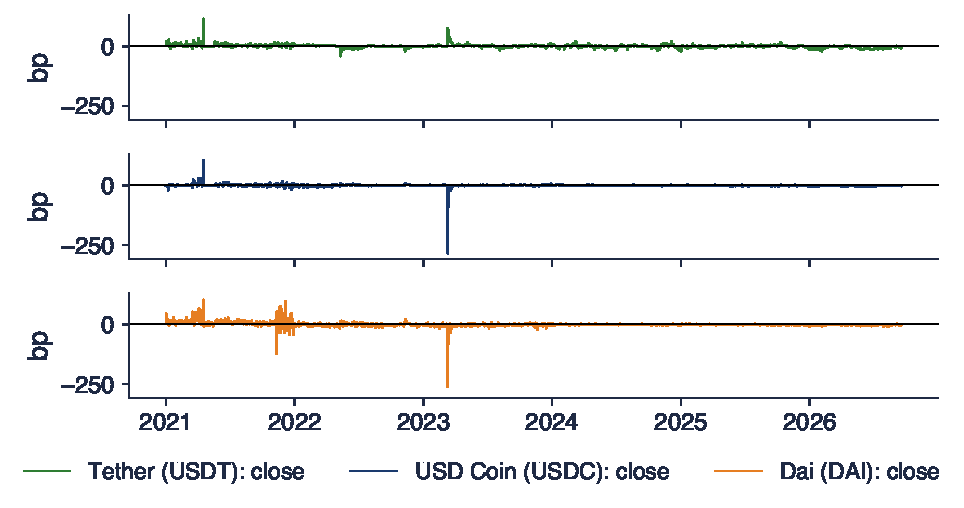
\includegraphics[width=0.97\textwidth,height=0.48\textheight,keepaspectratio]{sfm_ch14_peg.pdf}
\end{center}
\vspace{-0.25cm}
\begin{itemize}
    \item Abaterea zilnică a închiderii de la 1 USD, în bp, din 2021 (EODHD)
    \item Abaterea absolută mediană: USDT 3{,}1 bp, USDC 1{,}1 bp, DAI 2{,}2 bp; zile peste 10 bp: 11{,}4\%; 1{,}5\%; 10{,}7\%
    \item Interpretare: timpi de înjumătățire de 2{,}2; 0{,}6 și 0{,}6 zile: abaterile se închid în cîteva zile; excepția este martie 2023 (USDC $-285$ bp, DAI $-261$ bp)
\end{itemize}
\sfmquantlet{Ch_14}{SFM_ch14_stablecoins}
\end{frame}

\begin{frame}{Martie 2023: USDC și Silicon Valley Bank}
\itemsize{\footnotesize}
\begin{columns}[T]
\begin{column}{0.62\textwidth}
\begin{itemize}
    \item 10 martie 2023: Silicon Valley Bank (SVB) este închisă de autoritatea de supraveghere \refFDIC; o parte din rezervele în numerar ale USDC erau depuse acolo
    \begin{itemize}
        \item urmează un weekend: băncile sînt închise, piețele cripto sînt deschise
    \end{itemize}
    \item 11 martie: USDC scade la 0{,}8774 USD (minim, $-1226$ bp) și se închide la 0{,}9715; DAI, garantat în mare parte cu USDC, îl urmează
    \begin{itemize}
        \item USDT se tranzacționează peste 1 (închidere de pînă la 77 bp): banii fug de la un stablecoin la altul
    \end{itemize}
    \item 12 martie, seara: autoritățile americane garantează toate depozitele SVB \refFed; pe 13 martie USDC revine la paritate
\end{itemize}
\end{column}
\begin{column}{0.35\textwidth}
\centering

\includegraphics[height=0.34\textheight]{ch14_svb_hq_2023.jpg}\\[1mm]
\imgcap{Sediul SVB, Santa Clara, 13 martie 2023}
\imgcredit{https://commons.wikimedia.org/wiki/File:3003_West_Tasman_Drive_entrance_2,_Santa_Clara,_California.jpg}{Foto: Minh Nguyen (2023); CC BY-SA 4.0; Wikimedia Commons}
\end{column}
\end{columns}
\end{frame}

\begin{frame}{Depeg-ul USDC, zi de zi}
\itemsize{\footnotesize}
\begin{center}
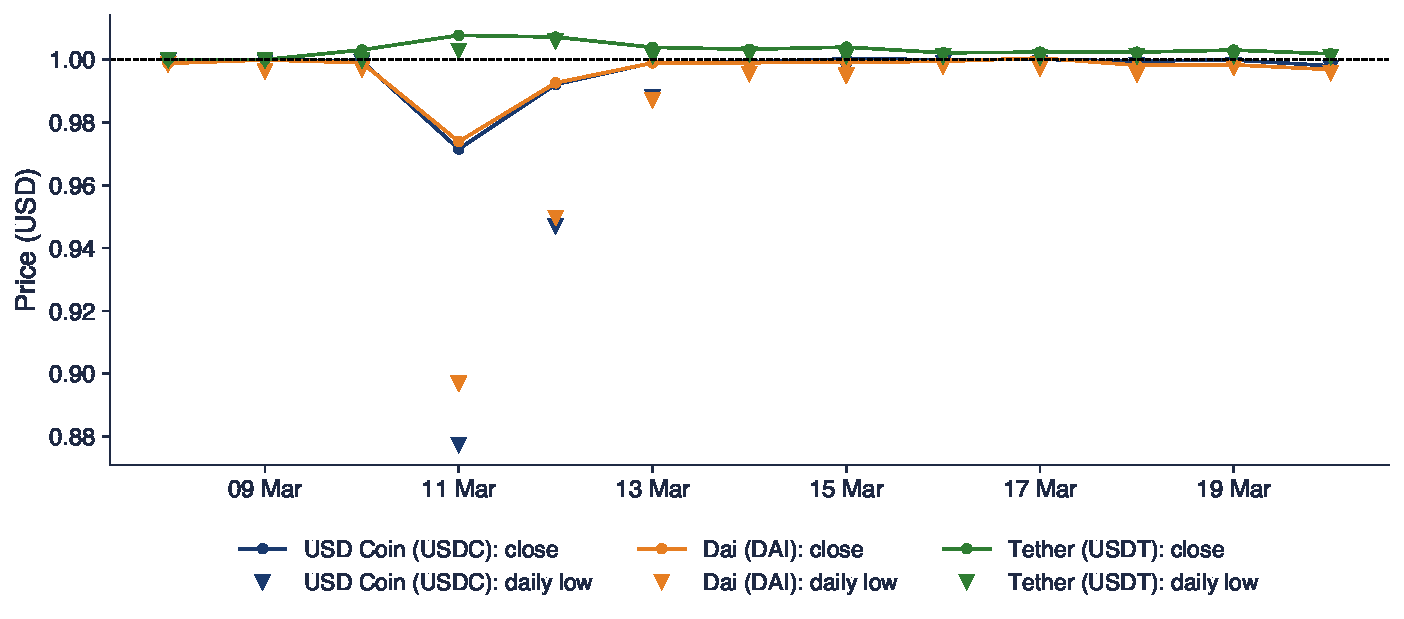
\includegraphics[width=0.97\textwidth,height=0.48\textheight,keepaspectratio]{sfm_ch14_svb.pdf}
\end{center}
\vspace{-0.25cm}
\begin{itemize}
    \item Închideri zilnice (cercuri) și minime (triunghiuri), 8--20 martie 2023; linia întreruptă: paritatea
    \item Interpretare: o monedă garantată fiat este la fel de sigură ca banca ei: paritatea s-a rupt cînd rezervele au fost puse sub semnul întrebării și a revenit cînd depozitele au fost garantate; retragerea a vizat rezervele, nu codul
\end{itemize}
\sfmquantlet{Ch_14}{SFM_ch14_stablecoins}
\end{frame}

\begin{frame}{TerraUSD: un stablecoin algoritmic}
\itemsize{\small}
\begin{itemize}
    \item UST era ținut la 1 USD printr-un schimb cu o a doua monedă, LUNA: 1 UST putea fi schimbat oricînd pe LUNA în valoare de 1 USD
    \begin{itemize}
        \item UST sub 1: cumpărăm UST, îl schimbăm pe LUNA nou de 1 USD, vindem LUNA: UST se arde, LUNA se emite
        \item singura garanție era valoarea de piață a LUNA
    \end{itemize}
    \item Cererea venea de la protocolul Anchor, care plătea aproape 20\% pe an pentru depozitele în UST \refLMS
    \begin{itemize}
        \item oferta de UST a atins maximul de 18{,}8 miliarde pe 7 mai 2022
    \end{itemize}
    \item \textbf{Spirala morții} (death spiral): retrageri mari din Anchor, UST sub 1, se emite mai mult LUNA, LUNA scade, garanția se micșorează, urmează și mai multe retrageri
    \begin{itemize}
        \item \refLMS: deținătorii mari și sofisticați s-au retras primii; deținătorii mici au plecat ultimii
    \end{itemize}
\end{itemize}
\end{frame}

\begin{frame}{Prăbușirea UST, mai 2022}
\itemsize{\footnotesize}
\begin{center}
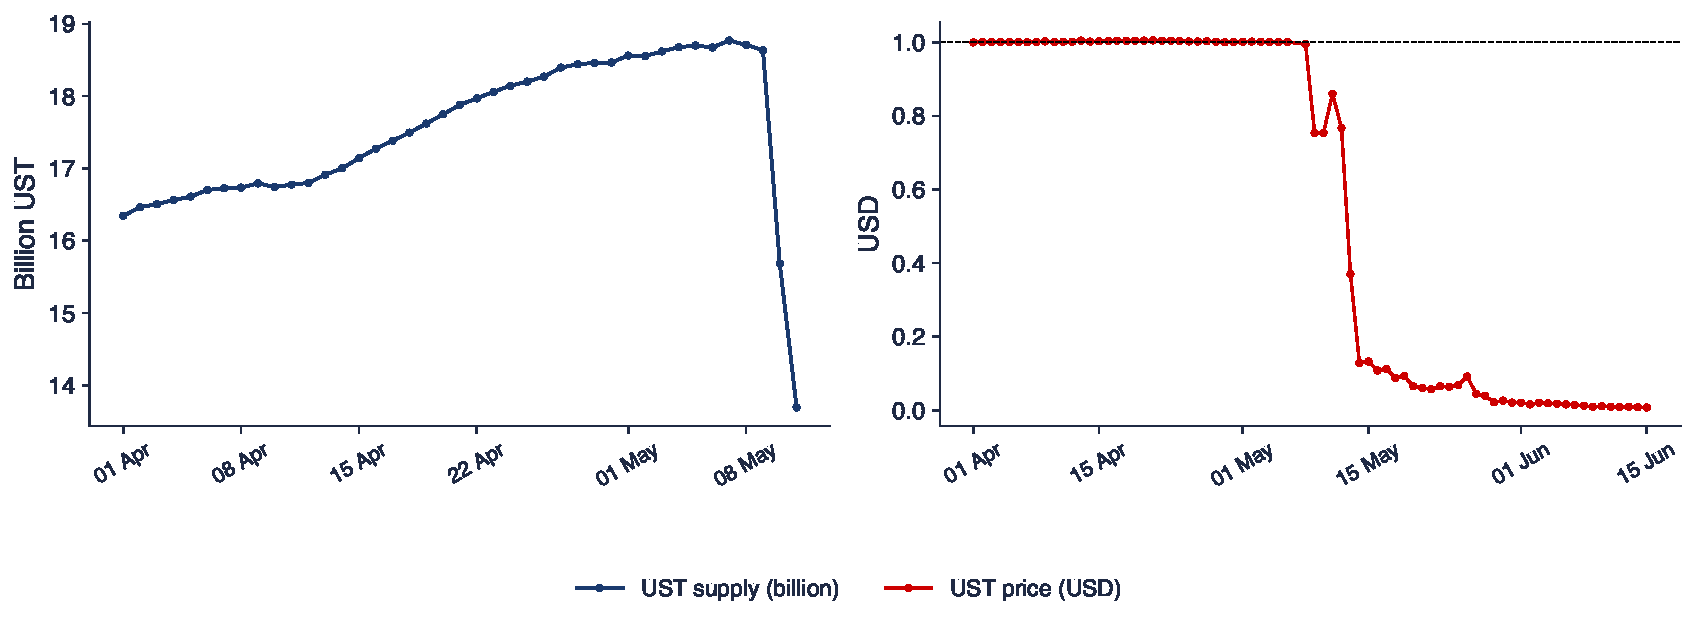
\includegraphics[width=0.97\textwidth,height=0.44\textheight,keepaspectratio]{sfm_ch14_ust.pdf}
\end{center}
\vspace{-0.25cm}
\begin{itemize}
    \item DefiLlama: oferta de UST pînă în ultima zi publicată (11 mai 2022) și prețul zilnic al UST
    \item Interpretare: prețul era 0{,}75 USD pe 9 mai, 0{,}37 pe 13 mai, 0{,}13 pe 14 mai și 0{,}02 pe 31 mai; oferta a scăzut cu 27\% în patru zile, între 7 și 11 mai
    \item Spre deosebire de USDC, nu exista nicio rezervă și niciun creditor de ultimă instanță: o paritate algoritmică nu poate fi salvată
\end{itemize}
\sfmquantlet{Ch_14}{SFM_ch14_stablecoins}
\end{frame}

\begin{frame}{Stablecoins ca monedă privată}
\itemsize{\small}
\begin{itemize}
    \item \refGZ: stablecoins seamănă cu bancnotele băncilor private americane din perioada „wildcat banking” (1837--1863)
    \begin{itemize}
        \item bancnotele diferitelor bănci se tranzacționau cu reduceri diferite, după încrederea în fiecare bancă
        \item remediul de atunci: o monedă națională uniformă; remediul propus acum: reglementarea stablecoins ca depozite bancare
    \end{itemize}
    \item \refGorton: paritatea se menține cîtă vreme deținătorii prețuiesc moneda pentru tranzacții cu levier pe piețele cripto
    \begin{itemize}
        \item cînd această cerere dispare, moneda se tranzacționează sub paritate, ca bancnota unei bănci nesigure
    \end{itemize}
    \item Lecția statistică: abaterile de la paritate sînt mici și scurte în perioadele normale și sar în criză: o serie cu cozi groase, dependentă de regim
\end{itemize}
\end{frame}

\begin{frame}{Reglementarea în Uniunea Europeană: MiCA}
\itemsize{\footnotesize}
\begin{columns}[T]
\begin{column}{0.62\textwidth}
\begin{itemize}
    \item MiCA, Markets in Crypto-Assets \refMiCA, adoptat în 2023
    \begin{itemize}
        \item regulile pentru stablecoins se aplică din 30 iunie 2024; pentru celelalte servicii cu active cripto din 30 decembrie 2024 \refESMA
    \end{itemize}
    \item Stablecoins legate de o singură monedă sînt \textbf{token-uri de monedă electronică} (e-money tokens)
    \begin{itemize}
        \item emise doar de instituții de credit sau de monedă electronică autorizate; răscumpărare la paritate oricînd; fără dobîndă pentru deținători
        \item rezervele sînt separate și investite în active sigure și lichide
    \end{itemize}
    \item Stablecoins algoritmice fără rezerve nu au loc în acest cadru
\end{itemize}
\end{column}
\begin{column}{0.35\textwidth}
\centering
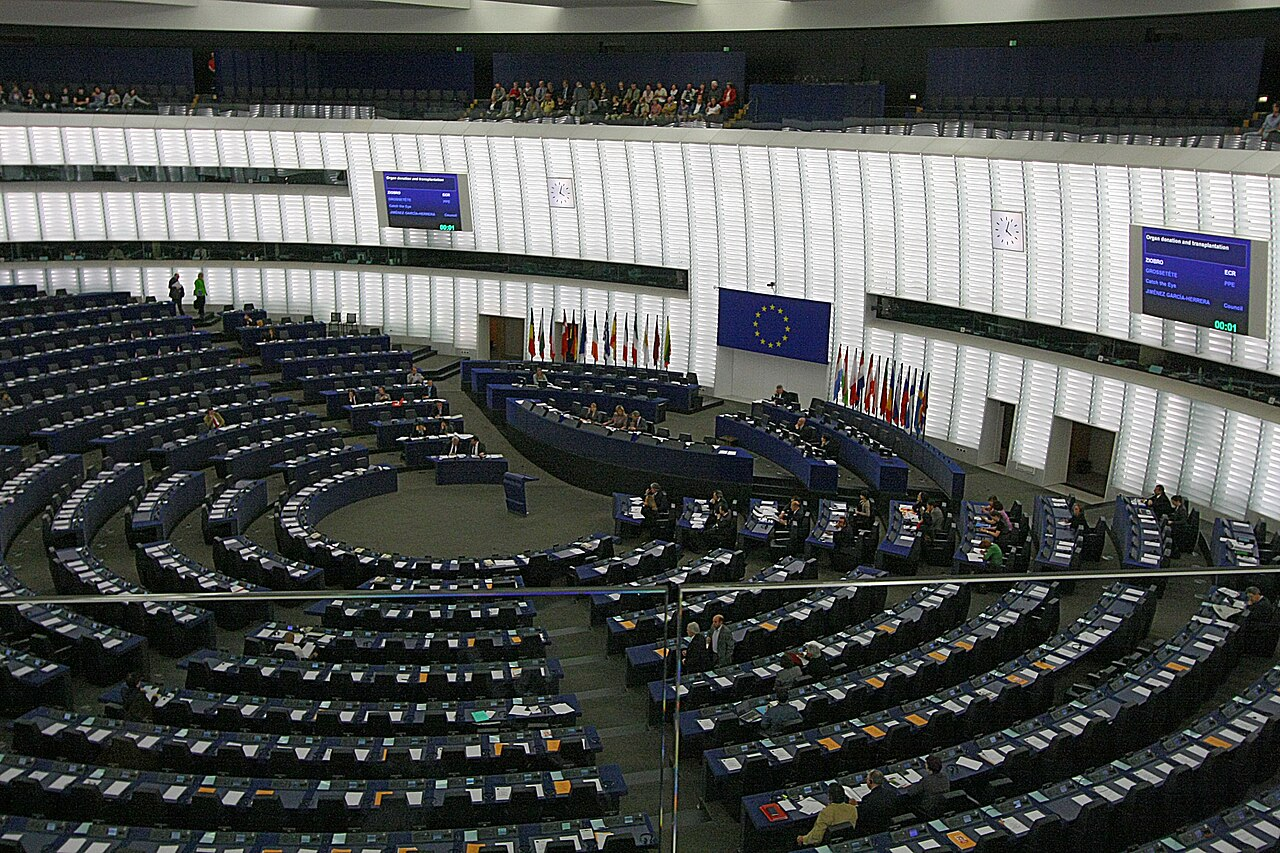
\includegraphics[height=0.30\textheight]{ch14_eu_parliament_2010.jpg}\\[1mm]
\imgcap{Parlamentul European, Strasbourg}
\imgcredit{https://commons.wikimedia.org/wiki/File:Hemicycle_of_Louise_Weiss_building_of_the_European_Parliament,_Strasbourg.jpg}{Foto: jeffowenphotos (2010); CC BY 2.0; Wikimedia Commons}
\end{column}
\end{columns}
\end{frame}

\begin{frame}{Reglementarea în SUA: GENIUS Act}
\itemsize{\footnotesize}
\begin{columns}[T]
\begin{column}{0.62\textwidth}
\begin{itemize}
    \item GENIUS Act (Guiding and Establishing National Innovation for U.S. Stablecoins Act), semnat pe 18 iulie 2025 \refGENIUS
    \begin{itemize}
        \item stablecoins de plată: rezerve de cel puțin 1 USD pentru fiecare monedă, în numerar, depozite și titluri de stat pe termen scurt
        \item rapoarte publice lunare despre rezerve; fără dobîndă plătită deținătorilor
    \end{itemize}
    \item Puncte comune ale MiCA și GENIUS: rezerve complete, răscumpărare la paritate, supravegherea emitenților
    \begin{itemize}
        \item răspund retragerii masive din martie 2023 și prăbușirii algoritmice din mai 2022
    \end{itemize}
    \item Un stablecoin cu rezerve complete este apropiat de o bancă îngustă (narrow bank): sigur, dar emitentul cîștigă dobînda la rezerve
\end{itemize}
\end{column}
\begin{column}{0.35\textwidth}
\centering
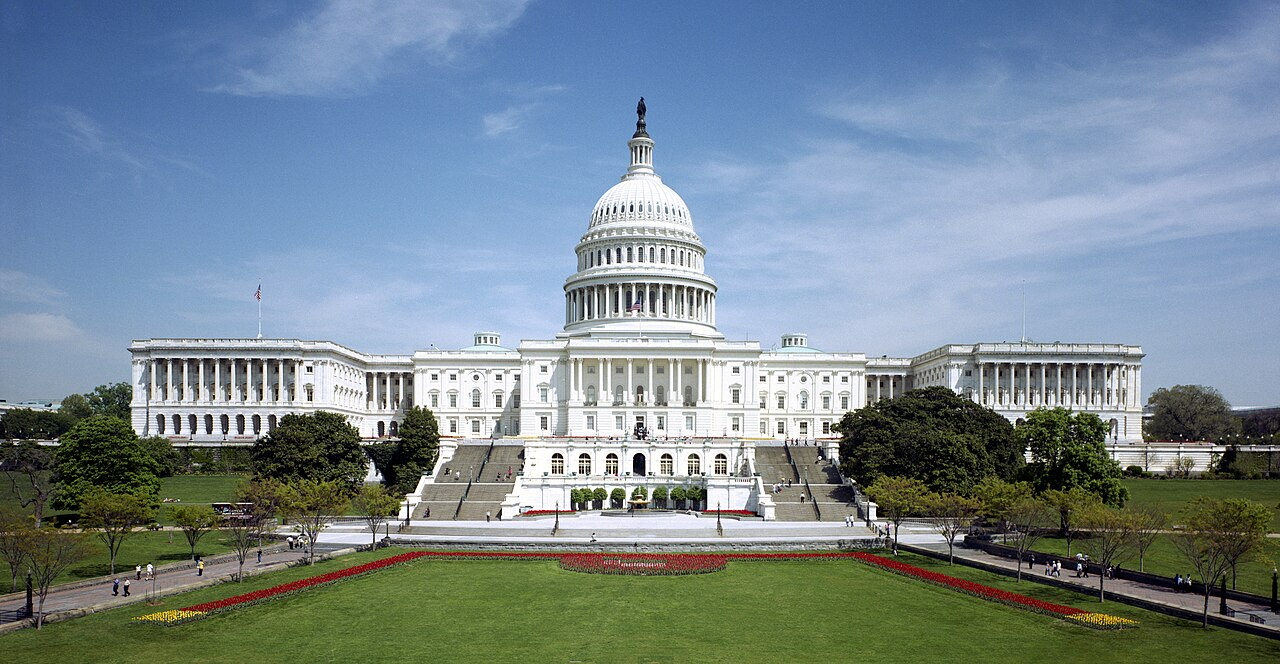
\includegraphics[height=0.24\textheight]{ch14_us_capitol.jpg}\\[1mm]
\imgcap{Capitoliul SUA, Washington, D.C.}
\imgcredit{https://commons.wikimedia.org/wiki/File:United_States_Capitol_-_west_front.jpg}{Foto: Architect of the Capitol; domeniu public; Wikimedia Commons}
\end{column}
\end{columns}
\end{frame}

\begin{frame}{Recapitulare: stablecoins}
\itemsize{\small}
\begin{itemize}
    \item Trei tipuri: garantate fiat, garantate cripto, algoritmice; o ofertă de 308 de miliarde USD în septembrie 2026
    \item Abaterea de la paritate în bp: $10\,000(P - 1)$; mică și de scurtă durată, cu excepția crizelor
    \item USDC (2023): o retragere masivă din cauza rezervelor, salvată; UST (2022): fără rezerve, prăbușire; MiCA și GENIUS cer rezerve complete
\end{itemize}
\end{frame}


%=============================================================================
\section{Riscul unei poziții cripto}
%=============================================================================

\begin{frame}{VaR 1\% și ES 2,5\% în dolari}
\itemsize{\small}
\begin{itemize}
    \item \sfmchlink{https://danpele.github.io/SFM/RO/Cursuri/capitol10_var_es_backtesting.pdf}{Capitolul 10}: $\mathrm{VaR}_\alpha = -q_\alpha$, pierderea depășită cu probabilitatea $\alpha$ (VaR 1\%); $\mathrm{ES}_\alpha = -E[r \mid r \le q_\alpha]$ (ES 2,5\%)
    \begin{itemize}
        \item simularea istorică (HS), distribuția Normală, Student-t (verosimilitate maximă), GARCH(1,1)-t pentru ziua următoare
    \end{itemize}
    \item De la randamente logaritmice la dolari: un randament logaritmic de $-v\%$ înseamnă o pierdere $W(1 - e^{-v/100})$ pentru o poziție cu valoarea $W$
    \begin{itemize}
        \item Bitcoin, HS: VaR 1\% $= 10{,}54\%$; $W = 100\,000$ USD: $100\,000 \times (1 - 0{,}8999) = 10\,006$ USD
    \end{itemize}
    \item Orizontul: activele cripto se tranzacționează zilnic, deci un VaR pe 10 zile acoperă 10 zile calendaristice, nu două săptămîni de tranzacționare
\end{itemize}
\end{frame}

\begin{frame}{Patru metode, trei active}
\itemsize{\scriptsize}
\begin{center}
\scriptsize
\begin{tabular}{lrrrrrrrr}
\toprule
& \multicolumn{4}{c}{VaR 1\% (\%)} & \multicolumn{4}{c}{ES 2,5\% (\%)} \\ & HS & Normală & t & GARCH-t & HS & Normală & t & GARCH-t \\
\midrule
Bitcoin & $10{,}54$ & $7{,}99$ & $11{,}06$ & $7{,}37$ & $10{,}84$ & $8{,}03$ & $13{,}37$ & $8{,}11$ \\
Ethereum & $14{,}29$ & $11{,}40$ & $15{,}39$ & $10{,}95$ & $14{,}77$ & $11{,}45$ & $18{,}13$ & $12{,}05$ \\
S\&P 500 & $3{,}26$ & $2{,}54$ & $3{,}04$ & $1{,}78$ & $3{,}50$ & $2{,}55$ & $3{,}45$ & $1{,}86$ \\
\bottomrule
\end{tabular}
\end{center}
\begin{center}
\scriptsize
\begin{tabular}{lrrrr}
\toprule
Poziție de 100\,000 USD & VaR 1\% HS & ES 2,5\% HS & VaR 1\% Normal & VaR 1\% HS pe 10 zile \\
\midrule
Bitcoin & 10\,006 & 10\,277 & 7\,679 & 25\,563 \\
Ethereum & 13\,312 & 13\,732 & 10\,772 & 31\,842 \\
S\&P 500 & 3\,204 & 3\,438 & 2\,506 & 9\,049 \\
\bottomrule
\end{tabular}
\end{center}
\begin{itemize}
    \item Eșantioanele complete pînă pe 18 septembrie 2026; t: Student-t prin verosimilitate maximă ($\hat\nu = 2{,}23$ pentru Bitcoin); GARCH-t: prognoza pentru ziua următoare ($\hat\sigma = 2{,}83\%$)
\end{itemize}
\end{frame}

\begin{frame}{Interpretarea cifrelor de risc}
\itemsize{\small}
\begin{itemize}
    \item O poziție în Bitcoin este de circa trei ori mai riscantă decît una în S\&P 500: VaR 1\% 10{,}54\% față de 3{,}26\%
    \begin{itemize}
        \item VaR 1\% Normal este cu 24\% sub cel istoric pentru Bitcoin: din nou cozile groase
    \end{itemize}
    \item Condiționat față de necondiționat: GARCH-t dă azi 7{,}37\%, sub valoarea istorică de 10{,}54\%, deoarece volatilitatea este acum scăzută
    \begin{itemize}
        \item cifra istorică este o medie pe termen lung; cifra GARCH este riscul de azi
    \end{itemize}
    \item 10 zile: VaR 1\% istoric al randamentelor pe 10 zile este 29{,}52\%; regula rădăcinii pătrate a timpului dă 33{,}34\%
    \begin{itemize}
        \item regula supraestimează: cu indicele de coadă $\alpha > 2$, o cuantilă extremă a sumei a $h$ randamente crește aproximativ ca $h^{1/\alpha}$, mai lent decît $\sqrt{h}$
    \end{itemize}
    \item ES 2,5\% (HS) este apropiat de VaR 1\% (HS) pentru Bitcoin, ca în \sfmchlink{https://danpele.github.io/SFM/RO/Cursuri/capitol10_var_es_backtesting.pdf}{Capitolul 10} pentru acțiuni
\end{itemize}
\end{frame}

\begin{frame}{Backtesting pentru VaR 1\% al Bitcoin}
\itemsize{\footnotesize}
\begin{center}
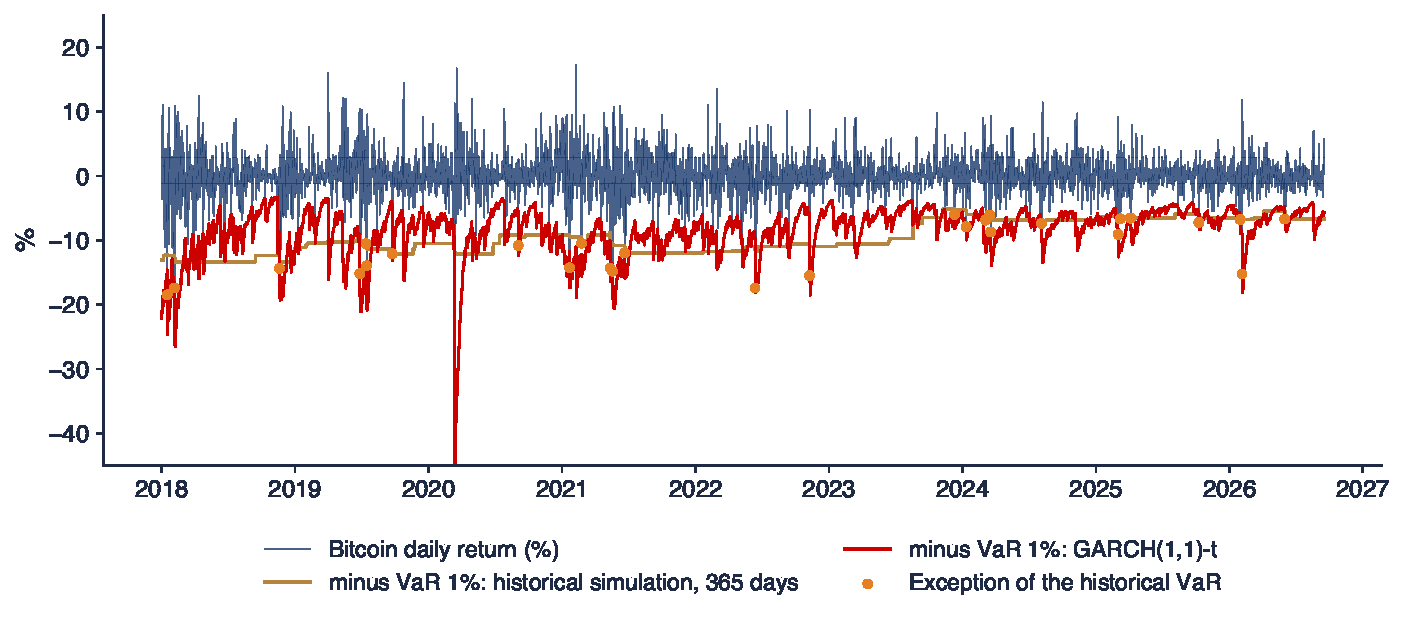
\includegraphics[width=0.97\textwidth,height=0.44\textheight,keepaspectratio]{sfm_ch14_btc_var.pdf}
\end{center}
\vspace{-0.25cm}
\begin{itemize}
    \item Prognoze pe o zi din 1 ianuarie 2018: HS pe ultimele 365 de zile; GARCH(1,1)-t reestimat la fiecare 365 de zile pe toate datele anterioare
    \item Depășiri (așteptat 31{,}8): HS 29 (0{,}91\%), GARCH-t 41 (1{,}29\%); Kupiec \refKupiec: $LR = 0{,}26$ (p $= 0{,}61$) și $2{,}45$ (p $= 0{,}12$)
    \item Interpretare: ambele trec testul Kupiec; HS cere în medie un VaR mai mare (9{,}5\% față de 8{,}5\%), GARCH-t reacționează mai repede, dar este depășit mai des (2018: 9 depășiri)
\end{itemize}
\sfmquantlet{Ch_14}{SFM_ch14_crypto_var}
\end{frame}

\begin{frame}{Recapitulare: riscul unei poziții cripto}
\itemsize{\small}
\begin{itemize}
    \item Convertim VaR din randamente logaritmice în bani cu $W(1 - e^{-v/100})$
    \item VaR 1\% al Bitcoin este de circa trei ori cel al S\&P 500; distribuția Normală îl subestimează
    \item Simularea istorică și GARCH-t trec amîndouă backtesting-ul din 2018
\end{itemize}
\end{frame}


%=============================================================================
\section{AI pentru descoperire științifică}
%=============================================================================

\begin{frame}{O întrebare deschisă}
\itemsize{\small}
\begin{itemize}
    \item \textbf{Influențează fluxurile de stablecoins prețurile activelor cripto?}
    \begin{itemize}
        \item \refGS{} au găsit că emisiunea de Tether a susținut Bitcoin în 2017; piața stablecoin-urilor este acum de circa 74 de ori mai mare decît în 2020
        \item rezultat de pornire: variația logaritmică săptămînală a ofertei de stablecoins față de randamentul Bitcoin, 349 de săptămîni din 2020
    \end{itemize}
    \item Aceeași săptămînă: corelația 0{,}26; săptămîna următoare: 0{,}07, panta 0{,}19 ($t = 1{,}20$, p $= 0{,}23$, $R^2 = 0{,}4\%$)
    \begin{itemize}
        \item fluxurile și prețurile se mișcă împreună; fluxurile nu prognozează săptămîna următoare: cauză, efect sau cerere comună?
    \end{itemize}
    \item Instrumentele AI pot accelera un astfel de studiu; nu înlocuiesc verificarea lui \refWang
\end{itemize}
\end{frame}

\begin{frame}{Contribuția posibilă a AI}
\itemsize{\small}
\begin{itemize}
    \item \textbf{Literatura}: o listă a studiilor despre emisiunea de stablecoins și prețurile cripto, cu datele și perioadele lor
    \item \textbf{Date}: cod care descarcă oferta fiecărui stablecoin de la DefiLlama și o aliniază cu prețurile zilnice
    \item \textbf{Robustețe}: date zilnice și săptămînale, USDT și USDC separat, subperioade, cauzalitate Granger în ambele direcții
    \item Exemplu de prompt
    \begin{itemize}
        \item \aiprompt{Write Python code that downloads the daily supply of USDT and USDC from the DefiLlama stablecoins API, computes weekly log changes, joins them with weekly Bitcoin log returns, and tests whether supply changes Granger-cause returns and returns Granger-cause supply changes, with HAC standard errors.}
    \end{itemize}
\end{itemize}
\end{frame}

\begin{frame}{Verificări necesare}
\itemsize{\small}
\begin{itemize}
    \item Anualizarea: 365 de zile pentru cripto, 252 pentru acțiuni; niciodată o singură valoare pentru ambele
    \item Alinierea: prețurile unite în zilele comune înainte de randamente; aceeași definiție a săptămînii pentru ambele serii
    \item Unitățile: puncte de bază față de procente (285 bp $= 2{,}85\%$); miliarde față de milioane în datele de ofertă
    \item Convenția VaR: VaR 1\% este o pierdere pozitivă; niciodată „VaR 99\%”
    \item Look-ahead: seria ofertei trebuie să fie cunoscută la data prognozei; revizuirile furnizorului de date contează
    \item Referințele: fiecare lucrare citată trebuie să existe; verificați DOI-ul
\end{itemize}
\end{frame}

\begin{frame}{Idee de proiect}
\itemsize{\small}
\begin{itemize}
    \item \textbf{Întrebarea}: ajută variațiile săptămînale ale ofertei de USDT și USDC la prognoza randamentului sau a volatilității Bitcoin și s-a schimbat acest lucru după ETF-urile spot?
    \begin{itemize}
        \item date: oferta de la DefiLlama (publică, fără cheie) și datele cursului pentru prețuri
    \end{itemize}
    \item Pași
    \begin{itemize}
        \item variații logaritmice săptămînale; corelația și testele Granger în ambele direcții, cu erori standard HAC
        \item prognoze în afara eșantionului pentru randamentul și pentru randamentul absolut din săptămîna următoare, comparate cu un mers aleator
        \item subperioade: înainte și după Terra (mai 2022) și ETF-urile spot (ianuarie 2024)
    \end{itemize}
    \item Livrabil: un tabel, un grafic și un paragraf despre ce pot și ce nu pot arăta datele
    \item Declarați orice utilizare a instrumentelor AI și enumerați erorile acestora pe care le-ați corectat
\end{itemize}
\end{frame}


%=============================================================================
\section{Rezumat}
%=============================================================================

\begin{frame}{Idei de reținut}
\itemsize{\small}
\begin{itemize}
    \item Bitcoin: un registru public securizat prin proof of work, cu o ofertă fixă de 21 de milioane; Ethereum execută contracte inteligente prin proof of stake
    \item Anualizăm cu 365 de zile; volatilitatea cripto este de 3{,}8 pînă la 6{,}7 ori cea a S\&P 500, cu cozi groase și grupare de tip IGARCH
    \item Testele VR robuste nu resping eficiența în formă slabă din 2014; weekendul este mai calm în varianță, nu diferit în medie
    \item Corelația cu acțiunile a crescut de la circa 0 la circa 0{,}39 după 2020; Bitcoin nu este un activ de refugiu
    \item Drawdown-urile de peste 50\% sînt obișnuite; efectul ETF-urilor asupra volatilității nu este semnificativ
    \item Stablecoins își mențin paritatea prin arbitraj și rezerve; USDC în 2023 și UST în 2022 arată cele două moduri în care se rupe o paritate
\end{itemize}
\end{frame}

\begin{frame}{Formule de reținut}
\itemsize{\small}
{\renewcommand{\arraystretch}{1.4}\begin{center}
\scriptsize
\begin{tabular}{ll}
\toprule
\textbf{Mărimea} & \textbf{Formula} \\
\midrule
Oferta de Bitcoin & $210\,000 \times 50 \times \sum_{j \ge 0} 2^{-j} = 21$ milioane \\
Anualizarea & media $m\bar r$, volatilitatea $\sqrt{m}\,s$; $m = 365$ (cripto), $252$ (acțiuni) \\
Hill & $\hat\alpha = \big[\frac1k\sum_{i \le k}\ln(X_{(i)}/X_{(k+1)})\big]^{-1}$ \\
GARCH(1,1) & $\sigma_t^2 = \omega + \alpha\varepsilon_{t-1}^2 + \beta\sigma_{t-1}^2$, înjumătățire $\frac{\ln 0{,}5}{\ln(\alpha + \beta)}$ \\
Raportul varianțelor & $\mathrm{VR}(q) = \mathrm{Var}(r_t + \dots + r_{t-q+1})/(q\,\mathrm{Var}(r_t))$ \\
Drawdown & $D_t = P_t/\max_{s \le t}P_s - 1$; cîștigul de recuperare $d/(1 - d)$ \\
Abaterea de la paritate & $d_t = 10\,000\,(P_t - 1)$ bp; înjumătățire $\ln 0{,}5/\ln\phi$ \\
VaR în bani & $W(1 - e^{-\mathrm{VaR}/100})$, $\mathrm{VaR}_\alpha = -q_\alpha$ \\
\bottomrule
\end{tabular}
\end{center}
}
\end{frame}

\begin{frame}{Autoevaluare}
\itemsize{\small}
\begin{itemize}
    \item \textbf{Întrebare}: un fond raportează o volatilitate anuală a Bitcoin de 55\% pornind de la o abatere standard zilnică de 3,5\%. Este corect?
    \begin{itemize}
        \item \textbf{Răspuns}: nu: $3{,}5 \times \sqrt{252} \approx 55{,}6\%$; cu 365 de zile se obține $3{,}5 \times \sqrt{365} \approx 66{,}9\%$
    \end{itemize}
    \item \textbf{Întrebare}: USDT se închide la 1,0040 USD. Cît este abaterea de la paritate?
    \begin{itemize}
        \item \textbf{Răspuns}: $10\,000 \times 0{,}0040 = 40$ bp peste paritate: cererea de USDT depășește ce a furnizat arbitrajul
    \end{itemize}
    \item \textbf{Întrebare}: de ce s-a pierdut UST, în timp ce USDC a revenit la paritate?
    \begin{itemize}
        \item \textbf{Răspuns}: USDC avea rezerve în dolari, ale căror depozite bancare au fost garantate; UST era garantat doar de LUNA, a cărei valoare a scăzut odată cu UST
    \end{itemize}
    \item Lecturi suplimentare ale autorului cursului: \refPeleA{} (sînt activele cripto active alternative?) și \refPeleB{} (VaR pentru Bitcoin)
    \item Urmează: \sfmchlink{https://danpele.github.io/SFM/RO/Cursuri/capitol15_risc_sistemic.pdf}{Capitolul 15}, riscul sistemic
\end{itemize}
\end{frame}


%=============================================================================
\section{Bibliografie}
%=============================================================================

\begin{frame}{Bibliografie (1/3)}
\itemsize{\tiny}
\begin{itemize}
    \item Baur, D.G., Hong, K., Lee, A.D. (2018). \href{https://doi.org/10.1016/j.intfin.2017.12.004}{Bitcoin: medium of exchange or speculative assets?} \textit{Journal of International Financial Markets, Institutions and Money}, 54, 177--189.
    \item Baur, D.G., Lucey, B.M. (2010). \href{https://doi.org/10.1111/j.1540-6288.2010.00244.x}{Is gold a hedge or a safe haven? An analysis of stocks, bonds and gold}. \textit{Financial Review}, 45(2), 217--229.
    \item Bollerslev, T. (1986). \href{https://doi.org/10.1016/0304-4076(86)90063-1}{Generalized autoregressive conditional heteroskedasticity}. \textit{Journal of Econometrics}, 31(3), 307--327.
    \item Buterin, V. (2014). \href{https://ethereum.org/en/whitepaper/}{Ethereum: a next-generation smart contract and decentralized application platform}. White paper.
    \item Caporale, G.M., Plastun, A. (2019). \href{https://doi.org/10.1016/j.frl.2018.11.012}{The day of the week effect in the cryptocurrency market}. \textit{Finance Research Letters}, 31, 258--269.
    \item Cheah, E.-T., Fry, J. (2015). \href{https://doi.org/10.1016/j.econlet.2015.02.029}{Speculative bubbles in Bitcoin markets? An empirical investigation into the fundamental value of Bitcoin}. \textit{Economics Letters}, 130, 32--36.
    \item European Union (2023). \href{https://eur-lex.europa.eu/eli/reg/2023/1114/oj}{Regulation (EU) 2023/1114 on markets in crypto-assets (MiCA)}. \textit{Official Journal of the European Union}, L 150, 40--205.
    \item Fama, E.F. (1970). \href{https://doi.org/10.2307/2325486}{Efficient capital markets: a review of theory and empirical work}. \textit{Journal of Finance}, 25(2), 383--417.
    \item Franke, J., Härdle, W.K., Hafner, C.M. (2019). \href{https://doi.org/10.1007/978-3-030-13751-9}{\textit{Statistics of Financial Markets: An Introduction}}, 5th ed. Springer.
    \item Gandal, N., Hamrick, J.T., Moore, T., Oberman, T. (2018). \href{https://doi.org/10.1016/j.jmoneco.2017.12.004}{Price manipulation in the Bitcoin ecosystem}. \textit{Journal of Monetary Economics}, 95, 86--96.
    \item Gorton, G.B., Klee, E.C., Ross, C.P., Ross, S.Y., Vardoulakis, A.P. (2022). \href{https://doi.org/10.3386/w30796}{Leverage and stablecoin pegs}. NBER Working Paper 30796.
    \item Gorton, G.B., Zhang, J. (2021). \href{https://doi.org/10.2139/ssrn.3888752}{Taming wildcat stablecoins}. SSRN Working Paper 3888752; published in \textit{University of Chicago Law Review}, 90(3), 2023.
    \item Griffin, J.M., Shams, A. (2020). \href{https://doi.org/10.1111/jofi.12903}{Is Bitcoin really untethered?} \textit{Journal of Finance}, 75(4), 1913--1964.
\end{itemize}
\end{frame}

\begin{frame}{Bibliografie (2/3)}
\itemsize{\tiny}
\begin{itemize}
    \item Hill, B.M. (1975). \href{https://doi.org/10.1214/aos/1176343247}{A simple general approach to inference about the tail of a distribution}. \textit{Annals of Statistics}, 3(5), 1163--1174.
    \item Härdle, W.K., Harvey, C.R., Reule, R.C.G. (2020). \href{https://doi.org/10.1093/jjfinec/nbz033}{Understanding cryptocurrencies}. \textit{Journal of Financial Econometrics}, 18(2), 181--208.
    \item Johansen, A., Ledoit, O., Sornette, D. (2000). \href{https://doi.org/10.1142/S0219024900000115}{Crashes as critical points}. \textit{International Journal of Theoretical and Applied Finance}, 3(2), 219--255.
    \item Katsiampa, P. (2017). \href{https://doi.org/10.1016/j.econlet.2017.06.023}{Volatility estimation for Bitcoin: a comparison of GARCH models}. \textit{Economics Letters}, 158, 3--6.
    \item Kupiec, P.H. (1995). \href{https://doi.org/10.3905/jod.1995.407942}{Techniques for verifying the accuracy of risk measurement models}. \textit{Journal of Derivatives}, 3(2), 73--84.
    \item Liu, J., Makarov, I., Schoar, A. (2023). \href{https://doi.org/10.3386/w31160}{Anatomy of a run: the Terra Luna crash}. NBER Working Paper 31160.
    \item Liu, Y., Tsyvinski, A. (2021). \href{https://doi.org/10.1093/rfs/hhaa113}{Risks and returns of cryptocurrency}. \textit{Review of Financial Studies}, 34(6), 2689--2727.
    \item Liu, Y., Tsyvinski, A., Wu, X. (2022). \href{https://doi.org/10.1111/jofi.13119}{Common risk factors in cryptocurrency}. \textit{Journal of Finance}, 77(2), 1133--1177.
    \item Lo, A.W., MacKinlay, A.C. (1988). \href{https://doi.org/10.1093/rfs/1.1.41}{Stock market prices do not follow random walks: evidence from a simple specification test}. \textit{Review of Financial Studies}, 1(1), 41--66.
    \item Lyons, R.K., Viswanath-Natraj, G. (2023). \href{https://doi.org/10.1016/j.jimonfin.2022.102777}{What keeps stablecoins stable?} \textit{Journal of International Money and Finance}, 131, 102777.
    \item Ma, Y., Zeng, Y., Zhang, A.L. (2025). \href{https://doi.org/10.3386/w33882}{Stablecoin runs and the centralization of arbitrage}. NBER Working Paper 33882.
    \item Makarov, I., Schoar, A. (2020). \href{https://doi.org/10.1016/j.jfineco.2019.07.001}{Trading and arbitrage in cryptocurrency markets}. \textit{Journal of Financial Economics}, 135(2), 293--319.
    \item Nadarajah, S., Chu, J. (2017). \href{https://doi.org/10.1016/j.econlet.2016.10.033}{On the inefficiency of Bitcoin}. \textit{Economics Letters}, 150, 6--9.
\end{itemize}
\end{frame}

\begin{frame}{Bibliografie (3/3)}
\itemsize{\tiny}
\begin{itemize}
    \item Nakamoto, S. (2008). \href{https://bitcoin.org/bitcoin.pdf}{Bitcoin: a peer-to-peer electronic cash system}. White paper.
    \item Pele, D.T., Mazurencu-Marinescu-Pele, M. (2019). \href{https://doi.org/10.3390/e21020102}{Using high-frequency entropy to forecast Bitcoin's daily value at risk}. \textit{Entropy}, 21(2), 102.
    \item Pele, D.T., Wesselhöfft, N., Härdle, W.K., Kolossiatis, M., Yatracos, Y.G. (2023). \href{https://doi.org/10.1080/1351847X.2021.1960403}{Are cryptos becoming alternative assets?} \textit{European Journal of Finance}, 29(10), 1064--1105.
    \item SEC, U.S. Securities and Exchange Commission (2024). \href{https://www.sec.gov/newsroom/speeches-statements/gensler-statement-spot-bitcoin-011023}{Statement on the approval of spot Bitcoin exchange-traded products}, 10 January 2024.
    \item Tran, V.L., Leirvik, T. (2020). \href{https://doi.org/10.1016/j.frl.2019.101382}{Efficiency in the markets of crypto-currencies}. \textit{Finance Research Letters}, 35, 101382.
    \item Treasury, Federal Reserve and FDIC (2023). \href{https://www.federalreserve.gov/newsevents/pressreleases/monetary20230312b.htm}{Joint statement by the Department of the Treasury, Federal Reserve, and FDIC}, 12 March 2023.
    \item Trimborn, S., Härdle, W.K. (2018). \href{https://doi.org/10.1016/j.jempfin.2018.08.004}{CRIX an index for cryptocurrencies}. \textit{Journal of Empirical Finance}, 49, 107--122.
    \item United States Congress (2025). \href{https://www.govinfo.gov/app/details/PLAW-119publ27}{Guiding and Establishing National Innovation for U.S. Stablecoins Act (GENIUS Act)}, Public Law 119-27.
    \item Urquhart, A. (2016). \href{https://doi.org/10.1016/j.econlet.2016.09.019}{The inefficiency of Bitcoin}. \textit{Economics Letters}, 148, 80--82.
    \item Wang, H., Fu, T., Du, Y., Gao, W., et al. (2023). \href{https://doi.org/10.1038/s41586-023-06221-2}{Scientific discovery in the age of artificial intelligence}. \textit{Nature}, 620, 47--60.
\end{itemize}
\end{frame}

\end{document}
